\documentclass[11pt]{article}
\usepackage[utf8]{inputenc}
\usepackage[T1]{fontenc}
\usepackage{textcomp}
\usepackage[a4paper,margin=2.1cm]{geometry}
\usepackage{amsmath,amssymb}
\usepackage{graphicx}
\usepackage{tikz}
\usetikzlibrary{arrows.meta}
\usepackage{xcolor}
\usepackage{mdframed}
\usepackage[colorlinks=true,linkcolor=blue!60!black]{hyperref}
\setlength{\parindent}{0pt}
\setlength{\parskip}{6pt}

\newcommand{\question}[1]{\par\medskip\noindent\textbf{#1}\par}
\newmdenv[linecolor=green!45!black,linewidth=0.8pt,backgroundcolor=green!4,
  innertopmargin=4pt,innerbottommargin=4pt,skipabove=6pt,skipbelow=6pt]{answerbox}

\title{\textbf{Parallel and Perpendicular Lines}\\[0.3em]\large Worked Solutions with TikZ Graphs}
\author{Wisest Maths --- Year 1 A-Level, Coordinate Geometry (ref \texttt{cg3})}
\date{}

\begin{document}
\maketitle
\noindent This document contains all 70 \emph{Parallel and Perpendicular Lines} questions, each with
a fully worked solution and (where a single plot is meaningful) a TikZ diagram on the coordinate plane:
the given line is drawn in grey and the answer line in blue, with parallel lines sharing a gradient and
perpendicular lines meeting at a right angle (the axes use equal scaling so right angles look right).
Perpendicular bisectors, altitudes, feet of perpendiculars, triangles and quadrilaterals are shown too.
\tableofcontents
\bigskip
\hrule

\section*{Parallel and Perpendicular Lines 01\quad\small\texttt{(cg3-001)}}
\addcontentsline{toc}{section}{Parallel and Perpendicular Lines 01 (cg3-001)}
\textit{Difficulty: Foundation \quad\textbar\quad Marks: 3}

\question{State which of the following lines are parallel to \( y = 4x - 3 \). \\[3pt] a) \( 2y = 8x + 5 \) b) \( y - 4x + 1 = 0 \) c) \( 8y + 32x = 1 \) d) \( \frac{1}{2}(y + 2) = 2x \) e) \( -12y - 3 = -48x \) f) \( 4y = x \)}

\textbf{Worked solution.}

\textit{Step 1: A line is parallel to \( y = 4x - 3 \) if and only if its gradient is \( 4 \). Rearrange each into \( y = mx + c \) form.}
\[\begin{gathered}
\text{a) } 2y = 8x + 5 \implies y = 4x + 2.5 \quad m = 4 \checkmark
\end{gathered}\]
Divide every term by \( 2 \) to isolate \( y \). The coefficient of \( x \) is the gradient.

\[\begin{gathered}
\text{b) } y = 4x - 1 \quad m = 4 \checkmark
\end{gathered}\]
Move \( -4x + 1 \) to the right-hand side: \( y = 4x - 1 \).

\[\begin{gathered}
\text{c) } 8y = -32x + 1 \implies y = -4x + \tfrac{1}{8} \quad m = -4 \times
\end{gathered}\]
Subtract \( 32x \) from both sides, then divide by \( 8 \). Gradient is \( -4 \), not \( 4 \), so not parallel.

\[\begin{gathered}
\text{d) } \tfrac{1}{2}y + 1 = 2x \implies y = 4x - 2 \quad m = 4 \checkmark
\end{gathered}\]
Distribute the \( \tfrac{1}{2} \) on the left to get \( \tfrac{1}{2}y + 1 = 2x \), then multiply through by \( 2 \) to clear the fraction.

\[\begin{gathered}
\text{e) } -12y = -48x + 3 \implies y = 4x - \tfrac{1}{4} \quad m = 4 \checkmark
\end{gathered}\]
Divide every term by \( -12 \). Be careful with signs: \( \tfrac{-48}{-12} = 4 \) and \( \tfrac{3}{-12} = -\tfrac{1}{4} \).

\[\begin{gathered}
\text{f) } y = \tfrac{1}{4}x \quad m = \tfrac{1}{4} \times
\end{gathered}\]
Divide both sides by \( 4 \). Gradient is \( \tfrac{1}{4} \), not \( 4 \) --- a common slip is to mix up \( 4y = x \) with \( y = 4x \).

\begin{answerbox}
\textbf{Final answer:}\quad Lines a), b), d) and e) are parallel to \(\displaystyle y = 4x - 3\).
\end{answerbox}
\textbf{Diagram.}

\begin{center}
\resizebox{\ifdim\width>\linewidth \linewidth\else \width\fi}{!}{%
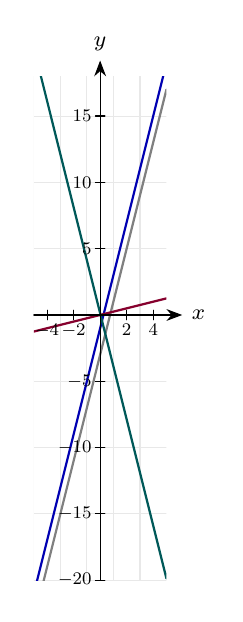
\begin{tikzpicture}[>={Stealth[length=2mm]},font=\footnotesize,line cap=round]
\begin{scope}
\clip (0,0) rectangle (1.684,6.4);
\draw[gray!18] (-0.168,0) grid[xstep=0.337,ystep=0.842] (1.684,6.4);
\draw[gray,thick] (0,-0.505) -- (1.684,6.232);
\draw[blue!70!black,thick] (0,-0.168) -- (1.684,6.568);
\draw[teal!70!black,thick] (0,6.758) -- (1.684,0.021);
\draw[purple!70!black,thick] (0,3.158) -- (1.684,3.579);
\end{scope}
\draw[->] (0,3.368) -- (1.884,3.368) node[right]{$x$};
\draw[->] (0.842,0) -- (0.842,6.6) node[above]{$y$};
\draw (0.168,3.308) -- (0.168,3.428) node[below=2pt,scale=0.8]{$-4$};
\draw (0.505,3.308) -- (0.505,3.428) node[below=2pt,scale=0.8]{$-2$};
\draw (1.179,3.308) -- (1.179,3.428) node[below=2pt,scale=0.8]{$2$};
\draw (1.516,3.308) -- (1.516,3.428) node[below=2pt,scale=0.8]{$4$};
\draw (0.782,0) -- (0.902,0) node[left=2pt,scale=0.8]{$-20$};
\draw (0.782,0.842) -- (0.902,0.842) node[left=2pt,scale=0.8]{$-15$};
\draw (0.782,1.684) -- (0.902,1.684) node[left=2pt,scale=0.8]{$-10$};
\draw (0.782,2.526) -- (0.902,2.526) node[left=2pt,scale=0.8]{$-5$};
\draw (0.782,4.211) -- (0.902,4.211) node[left=2pt,scale=0.8]{$5$};
\draw (0.782,5.053) -- (0.902,5.053) node[left=2pt,scale=0.8]{$10$};
\draw (0.782,5.895) -- (0.902,5.895) node[left=2pt,scale=0.8]{$15$};
\end{tikzpicture}
}
\end{center}
\small The line(s) and key points shown on the coordinate plane.\normalsize

\medskip\hrule

\section*{Parallel and Perpendicular Lines 02\quad\small\texttt{(cg3-002)}}
\addcontentsline{toc}{section}{Parallel and Perpendicular Lines 02 (cg3-002)}
\textit{Difficulty: Foundation \quad\textbar\quad Marks: 4}

\question{State whether each pair of lines is parallel, perpendicular, or neither. \\[3pt] a) \( y = 3x + 1 \) and \( y = 3x - 5 \) b) \( y = 2x + 4 \) and \( y = -\dfrac{1}{2}x + 1 \) c) \( y = 5x - 2 \) and \( y = -5x + 2 \) d) \( 2x - 4y + 3 = 0 \) and \( x - 2y - 1 = 0 \)}

\textbf{Worked solution.}

\textit{Step 1: Compare gradients. Two lines are parallel if \( m_1 = m_2 \); perpendicular if \( m_1 \times m_2 = -1 \).}
\[\begin{gathered}
\text{a) } m_1 = 3,\ m_2 = 3 \implies \textbf{parallel}
\end{gathered}\]
Both lines are already in \( y = mx + c \) form, so the gradients can be read straight off. Equal gradients (and different intercepts) means parallel.

\[\begin{gathered}
\text{b) } m_1 = 2,\ m_2 = -\tfrac{1}{2},\ 2 \times (-\tfrac{1}{2}) = -1 \implies \textbf{perpendicular}
\end{gathered}\]
\( -\tfrac{1}{2} \) is the negative reciprocal of \( 2 \), so the product of gradients is \( -1 \) --- the perpendicularity condition.

\[\begin{gathered}
\text{c) } m_1 = 5,\ m_2 = -5,\ 5 \times (-5) = -25 \ne -1 \implies \textbf{neither}
\end{gathered}\]
A common mistake is to assume that opposite signs alone imply perpendicularity. For perpendicular lines you need the negative \textbackslash emph\{reciprocal\} (here \( -\tfrac{1}{5} \)), not just the negative.

\textit{Step 4: Rearrange part d): both give \( m = \frac{1}{2} \).}
\[\begin{gathered}
2x - 4y + 3 = 0 \implies y = \tfrac{1}{2}x + \tfrac{3}{4}; \quad x - 2y - 1 = 0 \implies y = \tfrac{1}{2}x - \tfrac{1}{2} \implies \textbf{parallel}
\end{gathered}\]
Isolate \( y \) in each equation by moving the \( x \) and constant terms across, then divide by the coefficient of \( y \). Equal gradients with different intercepts confirm parallel.

\begin{answerbox}
\textbf{Final answer:}\quad a) Parallel; b) Perpendicular; c) Neither; d) Parallel
\end{answerbox}
\medskip\hrule

\section*{Parallel and Perpendicular Lines 03\quad\small\texttt{(cg3-003)}}
\addcontentsline{toc}{section}{Parallel and Perpendicular Lines 03 (cg3-003)}
\textit{Difficulty: Foundation \quad\textbar\quad Marks: 3}

\question{State whether each pair of lines is parallel, perpendicular, or neither. \\[3pt] a) \( 3x + y - 4 = 0 \) and \( 6x + 2y + 1 = 0 \) b) \( 4x - y + 2 = 0 \) and \( x + 4y - 8 = 0 \) c) \( 2x + 5y - 10 = 0 \) and \( 5x - 2y + 3 = 0 \)}

\textbf{Worked solution.}

\textit{Step 1: Rearrange to find gradients.}
\[\begin{gathered}
\text{a) } y = -3x + 4 \text{ and } y = -3x - \tfrac{1}{2} \implies m_1 = m_2 = -3 \implies \textbf{parallel}
\end{gathered}\]
For the general form \( Ax + By + C = 0 \) the gradient is \( -\tfrac{A}{B} \). Both lines give \( m = -3 \), so they are parallel.

\[\begin{gathered}
\text{b) } y = 4x + 2 \text{ and } y = -\tfrac{1}{4}x + 2 \implies 4 \times (-\tfrac{1}{4}) = -1 \implies \textbf{perpendicular}
\end{gathered}\]
\( -\tfrac{1}{4} \) is the negative reciprocal of \( 4 \), so the product is \( -1 \). Note both lines pass through \( (0, 2) \), so they meet at a right angle there.

\[\begin{gathered}
\text{c) } y = -\tfrac{2}{5}x + 2 \text{ and } y = \tfrac{5}{2}x + \tfrac{3}{2} \implies (-\tfrac{2}{5}) \times \tfrac{5}{2} = -1 \implies \textbf{perpendicular}
\end{gathered}\]
The gradients \( -\tfrac{2}{5} \) and \( \tfrac{5}{2} \) are negative reciprocals (flip the fraction and swap sign), so their product is \( -1 \).

\begin{answerbox}
\textbf{Final answer:}\quad a) Parallel; b) Perpendicular; c) Perpendicular
\end{answerbox}
\medskip\hrule

\section*{Parallel and Perpendicular Lines 04\quad\small\texttt{(cg3-004)}}
\addcontentsline{toc}{section}{Parallel and Perpendicular Lines 04 (cg3-004)}
\textit{Difficulty: Foundation \quad\textbar\quad Marks: 3}

\question{Find the value of \( k \) so that the line \( kx + 3y - 5 = 0 \) is parallel to \( y = 4x - 2 \).}

\textbf{Worked solution.}

\textit{Step 1: Rearrange \( kx + 3y - 5 = 0 \) to find its gradient.}
\[\begin{gathered}
3y = -kx + 5 \implies y = -\dfrac{k}{3}x + \dfrac{5}{3}
\end{gathered}\]
Move the \( x \) and constant terms to the right, then divide through by the coefficient of \( y \). The coefficient of \( x \) is the gradient, here \( -\tfrac{k}{3} \).

\textit{Step 2: For parallel lines, set gradients equal: \( -\dfrac{k}{3} = 4 \).}
\[\begin{gathered}
-\dfrac{k}{3} = 4 \implies k = -12
\end{gathered}\]
Multiply both sides by \( -3 \). Watch the sign --- multiplying by a negative flips the right-hand side from \( 4 \) to \( -12 \).

\begin{answerbox}
\textbf{Final answer:}\quad \(\displaystyle k = -12\)
\end{answerbox}
\textbf{Diagram.}

\begin{center}
\resizebox{\ifdim\width>\linewidth \linewidth\else \width\fi}{!}{%
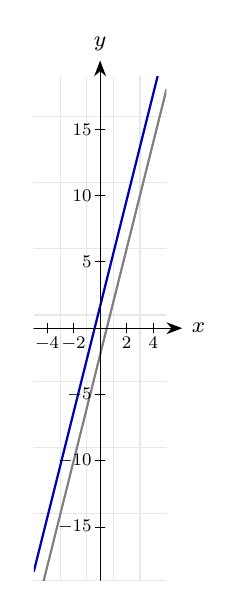
\begin{tikzpicture}[>={Stealth[length=2mm]},font=\footnotesize,line cap=round]
\begin{scope}
\clip (0,0) rectangle (1.684,6.4);
\draw[gray!18] (-0.168,-0.168) grid[xstep=0.337,ystep=0.842] (1.684,6.4);
\draw[gray,thick] (0,-0.505) -- (1.684,6.232);
\draw[blue!70!black,thick] (0,0.112) -- (1.684,6.849);
\end{scope}
\draw[->] (0,3.2) -- (1.884,3.2) node[right]{$x$};
\draw[->] (0.842,0) -- (0.842,6.6) node[above]{$y$};
\draw (0.168,3.14) -- (0.168,3.26) node[below=2pt,scale=0.8]{$-4$};
\draw (0.505,3.14) -- (0.505,3.26) node[below=2pt,scale=0.8]{$-2$};
\draw (1.179,3.14) -- (1.179,3.26) node[below=2pt,scale=0.8]{$2$};
\draw (1.516,3.14) -- (1.516,3.26) node[below=2pt,scale=0.8]{$4$};
\draw (0.782,0.674) -- (0.902,0.674) node[left=2pt,scale=0.8]{$-15$};
\draw (0.782,1.516) -- (0.902,1.516) node[left=2pt,scale=0.8]{$-10$};
\draw (0.782,2.358) -- (0.902,2.358) node[left=2pt,scale=0.8]{$-5$};
\draw (0.782,4.042) -- (0.902,4.042) node[left=2pt,scale=0.8]{$5$};
\draw (0.782,4.884) -- (0.902,4.884) node[left=2pt,scale=0.8]{$10$};
\draw (0.782,5.726) -- (0.902,5.726) node[left=2pt,scale=0.8]{$15$};
\end{tikzpicture}
}
\end{center}
\small The line(s) and key points shown on the coordinate plane.\normalsize

\medskip\hrule

\section*{Parallel and Perpendicular Lines 05\quad\small\texttt{(cg3-005)}}
\addcontentsline{toc}{section}{Parallel and Perpendicular Lines 05 (cg3-005)}
\textit{Difficulty: Foundation \quad\textbar\quad Marks: 3}

\question{Find the equation of the line parallel to \( y = 3x - 1 \) that passes through \( (2, 8) \). Give your answer in the form \( y = mx + c \).}

\textbf{Worked solution.}

\textit{Step 1: The gradient of the parallel line is \( m = 3 \). Write \( y = 3x + c \).}
\[\begin{gathered}
y = 3x + c
\end{gathered}\]
Parallel lines share the same gradient.

\textit{Step 2: Substitute \( (2, 8) \) to find \( c \).}
\[\begin{gathered}
8 = 3(2) + c \implies c = 2
\end{gathered}\]
The line must pass through \( (2, 8) \), so these coordinates satisfy the equation. Solve for \( c \) to pin down the \( y \)-intercept.

\textit{Step 3: Write the equation.}
\[\begin{gathered}
y = 3x + 2
\end{gathered}\]
Substitute the gradient and \( c \) back into \( y = mx + c \).

\begin{answerbox}
\textbf{Final answer:}\quad \(\displaystyle y = 3x + 2\)
\end{answerbox}
\textbf{Diagram.}

\begin{center}
\resizebox{\ifdim\width>\linewidth \linewidth\else \width\fi}{!}{%
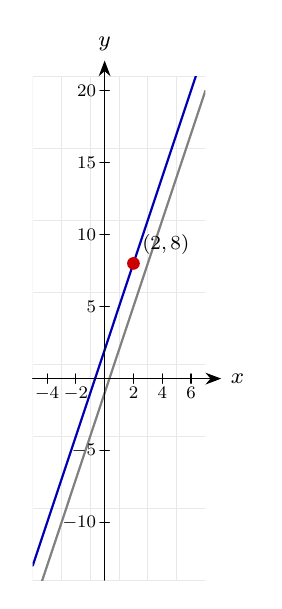
\begin{tikzpicture}[>={Stealth[length=2mm]},font=\footnotesize,line cap=round]
\begin{scope}
\clip (0,0) rectangle (2.194,6.4);
\draw[gray!18] (-0.183,-0.183) grid[xstep=0.366,ystep=0.914] (2.194,6.4);
\draw[gray,thick] (0,-0.366) -- (2.194,6.217);
\draw[blue!70!black,thick] (0,0.183) -- (2.194,6.766);
\end{scope}
\draw[->] (0,2.56) -- (2.394,2.56) node[right]{$x$};
\draw[->] (0.914,0) -- (0.914,6.6) node[above]{$y$};
\draw (0.183,2.5) -- (0.183,2.62) node[below=2pt,scale=0.8]{$-4$};
\draw (0.549,2.5) -- (0.549,2.62) node[below=2pt,scale=0.8]{$-2$};
\draw (1.28,2.5) -- (1.28,2.62) node[below=2pt,scale=0.8]{$2$};
\draw (1.646,2.5) -- (1.646,2.62) node[below=2pt,scale=0.8]{$4$};
\draw (2.011,2.5) -- (2.011,2.62) node[below=2pt,scale=0.8]{$6$};
\draw (0.854,0.731) -- (0.974,0.731) node[left=2pt,scale=0.8]{$-10$};
\draw (0.854,1.646) -- (0.974,1.646) node[left=2pt,scale=0.8]{$-5$};
\draw (0.854,3.474) -- (0.974,3.474) node[left=2pt,scale=0.8]{$5$};
\draw (0.854,4.389) -- (0.974,4.389) node[left=2pt,scale=0.8]{$10$};
\draw (0.854,5.303) -- (0.974,5.303) node[left=2pt,scale=0.8]{$15$};
\draw (0.854,6.217) -- (0.974,6.217) node[left=2pt,scale=0.8]{$20$};
\fill[red!80!black] (1.28,4.023) circle (2.3pt);
\node[above right,scale=0.9] at (1.28,4.023) {$(2,8)$};
\end{tikzpicture}
}
\end{center}
\small The line(s) and key points shown on the coordinate plane.\normalsize

\medskip\hrule

\section*{Parallel and Perpendicular Lines 06\quad\small\texttt{(cg3-006)}}
\addcontentsline{toc}{section}{Parallel and Perpendicular Lines 06 (cg3-006)}
\textit{Difficulty: Foundation \quad\textbar\quad Marks: 4}

\question{Find the equation of the line parallel to \( y = -2x + 5 \) passing through \( (3, 1) \). Give your answer in the form \( ax + by + c = 0 \).}

\textbf{Worked solution.}

\textit{Step 1: The gradient is \( m = -2 \). Use \( y = -2x + c \) and substitute \( (3, 1) \).}
\[\begin{gathered}
1 = -2(3) + c \implies c = 7
\end{gathered}\]
Parallel lines share gradients, so \( m = -2 \). Plug the given point in to solve for \( c \): \( 1 = -6 + c \) gives \( c = 7 \).

\textit{Step 2: Rearrange \( y = -2x + 7 \) into \( ax + by + c = 0 \).}
\[\begin{gathered}
2x + y - 7 = 0
\end{gathered}\]
Move every term to one side. Conventionally we take the coefficient of \( x \) positive, so add \( 2x \) and subtract \( 7 \) from both sides.

\begin{answerbox}
\textbf{Final answer:}\quad \(\displaystyle 2x + y - 7 = 0\)
\end{answerbox}
\textbf{Diagram.}

\begin{center}
\resizebox{\ifdim\width>\linewidth \linewidth\else \width\fi}{!}{%
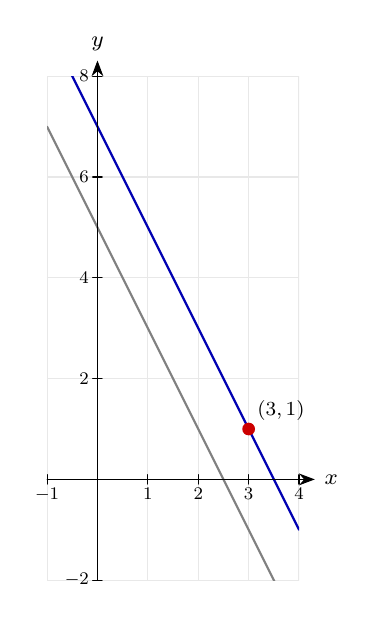
\begin{tikzpicture}[>={Stealth[length=2mm]},font=\footnotesize,line cap=round]
\begin{scope}
\clip (0,0) rectangle (3.2,6.4);
\draw[gray!18] (0,0) grid[xstep=0.64,ystep=1.28] (3.2,6.4);
\draw[gray,thick] (0,5.76) -- (3.2,-0.64);
\draw[blue!70!black,thick] (0,7.04) -- (3.2,0.64);
\end{scope}
\draw[->] (0,1.28) -- (3.4,1.28) node[right]{$x$};
\draw[->] (0.64,0) -- (0.64,6.6) node[above]{$y$};
\draw (0,1.22) -- (0,1.34) node[below=2pt,scale=0.8]{$-1$};
\draw (1.28,1.22) -- (1.28,1.34) node[below=2pt,scale=0.8]{$1$};
\draw (1.92,1.22) -- (1.92,1.34) node[below=2pt,scale=0.8]{$2$};
\draw (2.56,1.22) -- (2.56,1.34) node[below=2pt,scale=0.8]{$3$};
\draw (3.2,1.22) -- (3.2,1.34) node[below=2pt,scale=0.8]{$4$};
\draw (0.58,0) -- (0.7,0) node[left=2pt,scale=0.8]{$-2$};
\draw (0.58,2.56) -- (0.7,2.56) node[left=2pt,scale=0.8]{$2$};
\draw (0.58,3.84) -- (0.7,3.84) node[left=2pt,scale=0.8]{$4$};
\draw (0.58,5.12) -- (0.7,5.12) node[left=2pt,scale=0.8]{$6$};
\draw (0.58,6.4) -- (0.7,6.4) node[left=2pt,scale=0.8]{$8$};
\fill[red!80!black] (2.56,1.92) circle (2.3pt);
\node[above right,scale=0.9] at (2.56,1.92) {$(3,1)$};
\end{tikzpicture}
}
\end{center}
\small The line(s) and key points shown on the coordinate plane.\normalsize

\medskip\hrule

\section*{Parallel and Perpendicular Lines 07\quad\small\texttt{(cg3-007)}}
\addcontentsline{toc}{section}{Parallel and Perpendicular Lines 07 (cg3-007)}
\textit{Difficulty: Foundation \quad\textbar\quad Marks: 4}

\question{Line \( L \) passes through \( (0, 5) \) and is parallel to \( 3x - 6y + 4 = 0 \). Find the equation of \( L \) in the form \( y = mx + c \).}

\textbf{Worked solution.}

\textit{Step 1: Rearrange \( 3x - 6y + 4 = 0 \) to find its gradient.}
\[\begin{gathered}
6y = 3x + 4 \implies y = \dfrac{1}{2}x + \dfrac{2}{3}
\end{gathered}\]
Gradient is \( m = \frac{1}{2} \).

\textit{Step 2: Since \( L \) passes through \( (0, 5) \), the \( y \)-intercept is 5.}
\[\begin{gathered}
y = \dfrac{1}{2}x + 5
\end{gathered}\]
When \( x = 0 \), \( y = c \), so \( c = 5 \) directly.

\begin{answerbox}
\textbf{Final answer:}\quad \(\displaystyle y = \dfrac{1}{2}x + 5\)
\end{answerbox}
\textbf{Diagram.}

\begin{center}
\resizebox{\ifdim\width>\linewidth \linewidth\else \width\fi}{!}{%
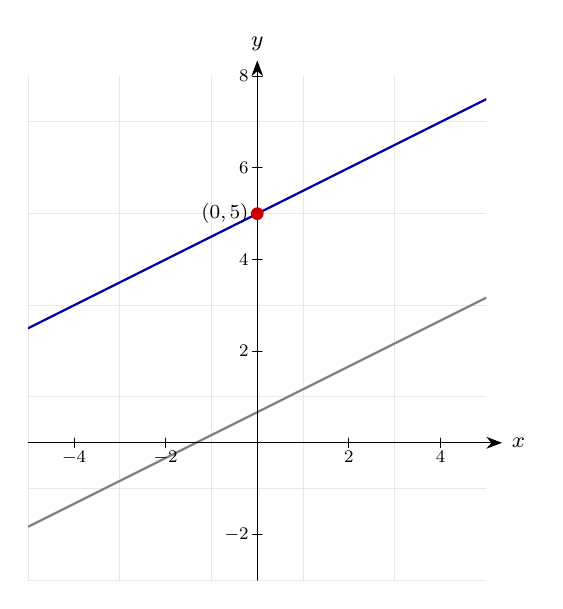
\begin{tikzpicture}[>={Stealth[length=2mm]},font=\footnotesize,line cap=round]
\begin{scope}
\clip (0,0) rectangle (5.818,6.4);
\draw[gray!18] (-0.582,-0.582) grid[xstep=1.164,ystep=1.164] (5.818,6.4);
\draw[gray,thick] (0,0.679) -- (5.818,3.588);
\draw[blue!70!black,thick] (0,3.2) -- (5.818,6.109);
\end{scope}
\draw[->] (0,1.745) -- (6.018,1.745) node[right]{$x$};
\draw[->] (2.909,0) -- (2.909,6.6) node[above]{$y$};
\draw (0.582,1.685) -- (0.582,1.805) node[below=2pt,scale=0.8]{$-4$};
\draw (1.745,1.685) -- (1.745,1.805) node[below=2pt,scale=0.8]{$-2$};
\draw (4.073,1.685) -- (4.073,1.805) node[below=2pt,scale=0.8]{$2$};
\draw (5.236,1.685) -- (5.236,1.805) node[below=2pt,scale=0.8]{$4$};
\draw (2.849,0.582) -- (2.969,0.582) node[left=2pt,scale=0.8]{$-2$};
\draw (2.849,2.909) -- (2.969,2.909) node[left=2pt,scale=0.8]{$2$};
\draw (2.849,4.073) -- (2.969,4.073) node[left=2pt,scale=0.8]{$4$};
\draw (2.849,5.236) -- (2.969,5.236) node[left=2pt,scale=0.8]{$6$};
\draw (2.849,6.4) -- (2.969,6.4) node[left=2pt,scale=0.8]{$8$};
\fill[red!80!black] (2.909,4.655) circle (2.3pt);
\node[left,scale=0.9] at (2.909,4.655) {$(0,5)$};
\end{tikzpicture}
}
\end{center}
\small The line(s) and key points shown on the coordinate plane.\normalsize

\medskip\hrule

\section*{Parallel and Perpendicular Lines 08\quad\small\texttt{(cg3-008)}}
\addcontentsline{toc}{section}{Parallel and Perpendicular Lines 08 (cg3-008)}
\textit{Difficulty: Foundation \quad\textbar\quad Marks: 4}

\question{Find the equation of the line parallel to \( 5x + 2y - 6 = 0 \) that passes through \( (4, -3) \). Give your answer in the form \( ax + by + c = 0 \), where \( a \), \( b \) and \( c \) are integers.}

\textbf{Worked solution.}

\textit{Step 1: Find the gradient of the given line.}
\[\begin{gathered}
2y = -5x + 6 \implies y = -\dfrac{5}{2}x + 3 \implies m = -\dfrac{5}{2}
\end{gathered}\]
Move the \( 5x \) and \( -6 \) across, then divide by \( 2 \). The parallel line will share this gradient.

\textit{Step 2: Use \( y = -\frac{5}{2}x + c \) with point \( (4, -3) \).}
\[\begin{gathered}
-3 = -\dfrac{5}{2}(4) + c \implies -3 = -10 + c \implies c = 7
\end{gathered}\]
Substitute the point into the parallel line equation. \( -\tfrac{5}{2} \times 4 = -10 \), then add \( 10 \) to both sides.

\textit{Step 3: Rearrange \( y = -\frac{5}{2}x + 7 \): multiply by 2.}
\[\begin{gathered}
2y = -5x + 14 \implies 5x + 2y - 14 = 0
\end{gathered}\]
Multiplying by \( 2 \) clears the fraction so the coefficients are integers, as required by the question.

\begin{answerbox}
\textbf{Final answer:}\quad \(\displaystyle 5x + 2y - 14 = 0\)
\end{answerbox}
\textbf{Diagram.}

\begin{center}
\resizebox{\ifdim\width>\linewidth \linewidth\else \width\fi}{!}{%
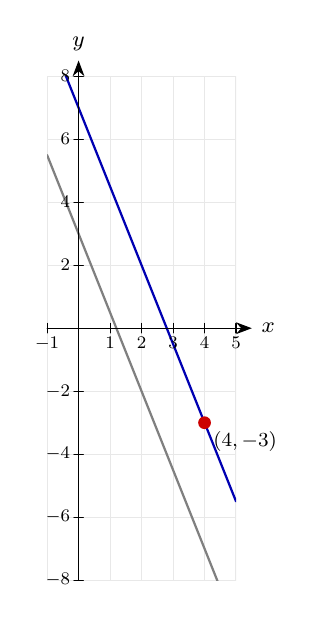
\begin{tikzpicture}[>={Stealth[length=2mm]},font=\footnotesize,line cap=round]
\begin{scope}
\clip (0,0) rectangle (2.4,6.4);
\draw[gray!18] (0,0) grid[xstep=0.4,ystep=0.8] (2.4,6.4);
\draw[gray,thick] (0,5.4) -- (2.4,-0.6);
\draw[blue!70!black,thick] (0,7) -- (2.4,1);
\end{scope}
\draw[->] (0,3.2) -- (2.6,3.2) node[right]{$x$};
\draw[->] (0.4,0) -- (0.4,6.6) node[above]{$y$};
\draw (0,3.14) -- (0,3.26) node[below=2pt,scale=0.8]{$-1$};
\draw (0.8,3.14) -- (0.8,3.26) node[below=2pt,scale=0.8]{$1$};
\draw (1.2,3.14) -- (1.2,3.26) node[below=2pt,scale=0.8]{$2$};
\draw (1.6,3.14) -- (1.6,3.26) node[below=2pt,scale=0.8]{$3$};
\draw (2,3.14) -- (2,3.26) node[below=2pt,scale=0.8]{$4$};
\draw (2.4,3.14) -- (2.4,3.26) node[below=2pt,scale=0.8]{$5$};
\draw (0.34,0) -- (0.46,0) node[left=2pt,scale=0.8]{$-8$};
\draw (0.34,0.8) -- (0.46,0.8) node[left=2pt,scale=0.8]{$-6$};
\draw (0.34,1.6) -- (0.46,1.6) node[left=2pt,scale=0.8]{$-4$};
\draw (0.34,2.4) -- (0.46,2.4) node[left=2pt,scale=0.8]{$-2$};
\draw (0.34,4) -- (0.46,4) node[left=2pt,scale=0.8]{$2$};
\draw (0.34,4.8) -- (0.46,4.8) node[left=2pt,scale=0.8]{$4$};
\draw (0.34,5.6) -- (0.46,5.6) node[left=2pt,scale=0.8]{$6$};
\draw (0.34,6.4) -- (0.46,6.4) node[left=2pt,scale=0.8]{$8$};
\fill[red!80!black] (2,2) circle (2.3pt);
\node[below right,scale=0.9] at (2,2) {$(4,-3)$};
\end{tikzpicture}
}
\end{center}
\small The line(s) and key points shown on the coordinate plane.\normalsize

\medskip\hrule

\section*{Parallel and Perpendicular Lines 09\quad\small\texttt{(cg3-009)}}
\addcontentsline{toc}{section}{Parallel and Perpendicular Lines 09 (cg3-009)}
\textit{Difficulty: Foundation \quad\textbar\quad Marks: 4}

\question{Find the equation of the line parallel to \( 4x - 3y + 9 = 0 \) passing through \( (-3, 2) \). Give your answer in the form \( ax + by + c = 0 \).}

\textbf{Worked solution.}

\textit{Step 1: Find gradient: \( 3y = 4x + 9 \implies m = \frac{4}{3} \).}
\[\begin{gathered}
m = \dfrac{4}{3}
\end{gathered}\]
Rearrange the given line into \( y = mx + c \) form by isolating \( y \). The parallel line will have the same gradient.

\textit{Step 2: Use \( y = \frac{4}{3}x + c \) with \( (-3, 2) \).}
\[\begin{gathered}
2 = \dfrac{4}{3}(-3) + c \implies 2 = -4 + c \implies c = 6
\end{gathered}\]
Substituting \( x = -3 \) into \( \tfrac{4}{3}x \) gives \( -4 \) (the \( 3 \)s cancel). Then \( c = 2 + 4 = 6 \).

\textit{Step 3: Rearrange \( y = \frac{4}{3}x + 6 \): multiply by 3.}
\[\begin{gathered}
3y = 4x + 18 \implies 4x - 3y + 18 = 0
\end{gathered}\]
Multiplying by \( 3 \) clears the fraction. Then bring everything to one side, keeping the \( x \)-coefficient positive.

\begin{answerbox}
\textbf{Final answer:}\quad \(\displaystyle 4x - 3y + 18 = 0\)
\end{answerbox}
\textbf{Diagram.}

\begin{center}
\resizebox{\ifdim\width>\linewidth \linewidth\else \width\fi}{!}{%
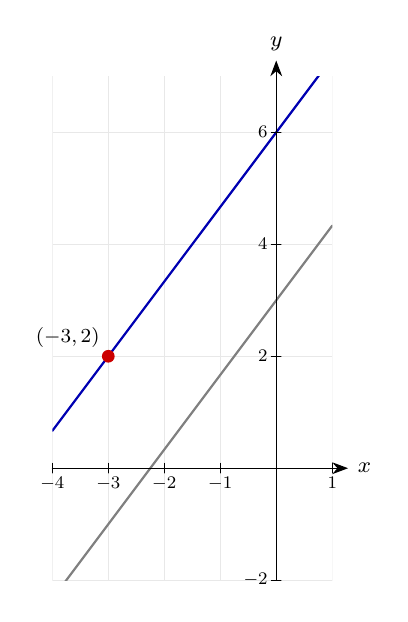
\begin{tikzpicture}[>={Stealth[length=2mm]},font=\footnotesize,line cap=round]
\begin{scope}
\clip (0,0) rectangle (3.556,6.4);
\draw[gray!18] (0,0) grid[xstep=0.711,ystep=1.422] (3.556,6.4);
\draw[gray,thick] (0,-0.237) -- (3.556,4.504);
\draw[blue!70!black,thick] (0,1.896) -- (3.556,6.637);
\end{scope}
\draw[->] (0,1.422) -- (3.756,1.422) node[right]{$x$};
\draw[->] (2.844,0) -- (2.844,6.6) node[above]{$y$};
\draw (0,1.362) -- (0,1.482) node[below=2pt,scale=0.8]{$-4$};
\draw (0.711,1.362) -- (0.711,1.482) node[below=2pt,scale=0.8]{$-3$};
\draw (1.422,1.362) -- (1.422,1.482) node[below=2pt,scale=0.8]{$-2$};
\draw (2.133,1.362) -- (2.133,1.482) node[below=2pt,scale=0.8]{$-1$};
\draw (3.556,1.362) -- (3.556,1.482) node[below=2pt,scale=0.8]{$1$};
\draw (2.784,0) -- (2.904,0) node[left=2pt,scale=0.8]{$-2$};
\draw (2.784,2.844) -- (2.904,2.844) node[left=2pt,scale=0.8]{$2$};
\draw (2.784,4.267) -- (2.904,4.267) node[left=2pt,scale=0.8]{$4$};
\draw (2.784,5.689) -- (2.904,5.689) node[left=2pt,scale=0.8]{$6$};
\fill[red!80!black] (0.711,2.844) circle (2.3pt);
\node[above left,scale=0.9] at (0.711,2.844) {$(-3,2)$};
\end{tikzpicture}
}
\end{center}
\small The line(s) and key points shown on the coordinate plane.\normalsize

\medskip\hrule

\section*{Parallel and Perpendicular Lines 10\quad\small\texttt{(cg3-010)}}
\addcontentsline{toc}{section}{Parallel and Perpendicular Lines 10 (cg3-010)}
\textit{Difficulty: Foundation \quad\textbar\quad Marks: 4}

\question{Line \( P \) passes through \( (6, -1) \) and is parallel to the line joining \( (0, 3) \) and \( (4, 11) \). Find the equation of \( P \) in the form \( y = mx + c \).}

\textbf{Worked solution.}

\textit{Step 1: Find the gradient of the line joining \( (0, 3) \) and \( (4, 11) \).}
\[\begin{gathered}
m = \dfrac{11 - 3}{4 - 0} = \dfrac{8}{4} = 2
\end{gathered}\]
Use the gradient formula \( m = \frac{y_2 - y_1}{x_2 - x_1} \). \( P \) is parallel to this line, so it shares the gradient.

\textit{Step 2: Use \( y = 2x + c \) with \( (6, -1) \).}
\[\begin{gathered}
-1 = 2(6) + c \implies c = -13
\end{gathered}\]
Substitute the point on \( P \). \( c = -1 - 12 = -13 \).

\textit{Step 3: Write the equation.}
\[\begin{gathered}
y = 2x - 13
\end{gathered}\]
Combine the gradient and \( y \)-intercept to give the final equation.

\begin{answerbox}
\textbf{Final answer:}\quad \(\displaystyle y = 2x - 13\)
\end{answerbox}
\textbf{Diagram.}

\begin{center}
\resizebox{\ifdim\width>\linewidth \linewidth\else \width\fi}{!}{%
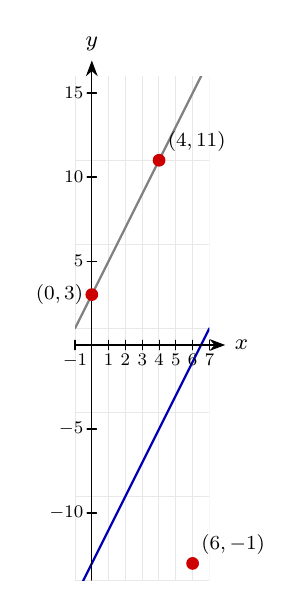
\begin{tikzpicture}[>={Stealth[length=2mm]},font=\footnotesize,line cap=round]
\begin{scope}
\clip (0,0) rectangle (1.707,6.4);
\draw[gray!18] (0,-0.213) grid[xstep=0.213,ystep=1.067] (1.707,6.4);
\draw[gray,thick] (0,3.2) -- (1.707,6.613);
\draw[blue!70!black,thick] (0,-0.213) -- (1.707,3.2);
\end{scope}
\draw[->] (0,2.987) -- (1.907,2.987) node[right]{$x$};
\draw[->] (0.213,0) -- (0.213,6.6) node[above]{$y$};
\draw (0,2.927) -- (0,3.047) node[below=2pt,scale=0.8]{$-1$};
\draw (0.427,2.927) -- (0.427,3.047) node[below=2pt,scale=0.8]{$1$};
\draw (0.64,2.927) -- (0.64,3.047) node[below=2pt,scale=0.8]{$2$};
\draw (0.853,2.927) -- (0.853,3.047) node[below=2pt,scale=0.8]{$3$};
\draw (1.067,2.927) -- (1.067,3.047) node[below=2pt,scale=0.8]{$4$};
\draw (1.28,2.927) -- (1.28,3.047) node[below=2pt,scale=0.8]{$5$};
\draw (1.493,2.927) -- (1.493,3.047) node[below=2pt,scale=0.8]{$6$};
\draw (1.707,2.927) -- (1.707,3.047) node[below=2pt,scale=0.8]{$7$};
\draw (0.153,0.853) -- (0.273,0.853) node[left=2pt,scale=0.8]{$-10$};
\draw (0.153,1.92) -- (0.273,1.92) node[left=2pt,scale=0.8]{$-5$};
\draw (0.153,4.053) -- (0.273,4.053) node[left=2pt,scale=0.8]{$5$};
\draw (0.153,5.12) -- (0.273,5.12) node[left=2pt,scale=0.8]{$10$};
\draw (0.153,6.187) -- (0.273,6.187) node[left=2pt,scale=0.8]{$15$};
\fill[red!80!black] (0.213,3.627) circle (2.3pt);
\node[left,scale=0.9] at (0.213,3.627) {$(0,3)$};
\fill[red!80!black] (1.067,5.333) circle (2.3pt);
\node[above right,scale=0.9] at (1.067,5.333) {$(4,11)$};
\fill[red!80!black] (1.493,0.213) circle (2.3pt);
\node[above right,scale=0.9] at (1.493,0.213) {$(6,-1)$};
\end{tikzpicture}
}
\end{center}
\small The line(s) and key points shown on the coordinate plane.\normalsize

\medskip\hrule

\section*{Parallel and Perpendicular Lines 11\quad\small\texttt{(cg3-011)}}
\addcontentsline{toc}{section}{Parallel and Perpendicular Lines 11 (cg3-011)}
\textit{Difficulty: Foundation \quad\textbar\quad Marks: 5}

\question{Find the equation of the line parallel to \( \dfrac{x}{3} + \dfrac{y}{2} = 1 \) that passes through \( (6, 5) \). Give your answer in the form \( ax + by + c = 0 \).}

\textbf{Worked solution.}

\textit{Step 1: Rearrange the given line to find its gradient.}
\[\begin{gathered}
\dfrac{x}{3} + \dfrac{y}{2} = 1 \implies 2x + 3y = 6 \implies y = -\dfrac{2}{3}x + 2
\end{gathered}\]
Multiply through by 6 to clear fractions, then isolate \( y \).

\textit{Step 2: The parallel line has gradient \( m = -\frac{2}{3} \). Substitute \( (6, 5) \).}
\[\begin{gathered}
5 = -\dfrac{2}{3}(6) + c \implies 5 = -4 + c \implies c = 9
\end{gathered}\]
\( -\tfrac{2}{3} \times 6 = -4 \) (the \( 3 \)s cancel). Then add \( 4 \) to both sides to find \( c \).

\textit{Step 3: Rearrange \( y = -\frac{2}{3}x + 9 \): multiply by 3.}
\[\begin{gathered}
3y = -2x + 27 \implies 2x + 3y - 27 = 0
\end{gathered}\]
Multiply by \( 3 \) to clear the fraction, then move all terms to one side to get the required integer-coefficient form.

\begin{answerbox}
\textbf{Final answer:}\quad \(\displaystyle 2x + 3y - 27 = 0\)
\end{answerbox}
\textbf{Diagram.}

\begin{center}
\resizebox{\ifdim\width>\linewidth \linewidth\else \width\fi}{!}{%
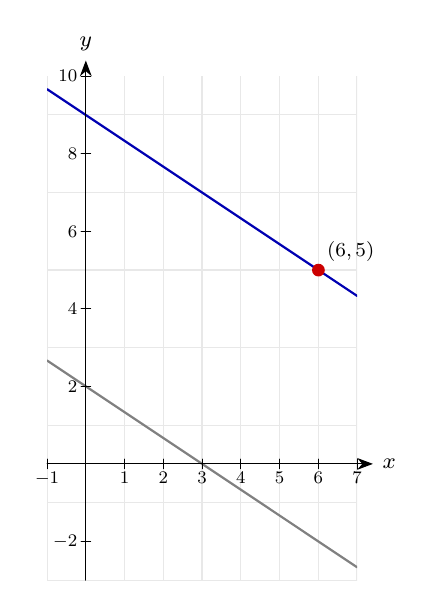
\begin{tikzpicture}[>={Stealth[length=2mm]},font=\footnotesize,line cap=round]
\begin{scope}
\clip (0,0) rectangle (3.938,6.4);
\draw[gray!18] (0,-0.492) grid[xstep=0.492,ystep=0.985] (3.938,6.4);
\draw[gray,thick] (0,2.79) -- (3.938,0.164);
\draw[blue!70!black,thick] (0,6.236) -- (3.938,3.61);
\end{scope}
\draw[->] (0,1.477) -- (4.138,1.477) node[right]{$x$};
\draw[->] (0.492,0) -- (0.492,6.6) node[above]{$y$};
\draw (0,1.417) -- (0,1.537) node[below=2pt,scale=0.8]{$-1$};
\draw (0.985,1.417) -- (0.985,1.537) node[below=2pt,scale=0.8]{$1$};
\draw (1.477,1.417) -- (1.477,1.537) node[below=2pt,scale=0.8]{$2$};
\draw (1.969,1.417) -- (1.969,1.537) node[below=2pt,scale=0.8]{$3$};
\draw (2.462,1.417) -- (2.462,1.537) node[below=2pt,scale=0.8]{$4$};
\draw (2.954,1.417) -- (2.954,1.537) node[below=2pt,scale=0.8]{$5$};
\draw (3.446,1.417) -- (3.446,1.537) node[below=2pt,scale=0.8]{$6$};
\draw (3.938,1.417) -- (3.938,1.537) node[below=2pt,scale=0.8]{$7$};
\draw (0.432,0.492) -- (0.552,0.492) node[left=2pt,scale=0.8]{$-2$};
\draw (0.432,2.462) -- (0.552,2.462) node[left=2pt,scale=0.8]{$2$};
\draw (0.432,3.446) -- (0.552,3.446) node[left=2pt,scale=0.8]{$4$};
\draw (0.432,4.431) -- (0.552,4.431) node[left=2pt,scale=0.8]{$6$};
\draw (0.432,5.415) -- (0.552,5.415) node[left=2pt,scale=0.8]{$8$};
\draw (0.432,6.4) -- (0.552,6.4) node[left=2pt,scale=0.8]{$10$};
\fill[red!80!black] (3.446,3.938) circle (2.3pt);
\node[above right,scale=0.9] at (3.446,3.938) {$(6,5)$};
\end{tikzpicture}
}
\end{center}
\small The line(s) and key points shown on the coordinate plane.\normalsize

\medskip\hrule

\section*{Parallel and Perpendicular Lines 12\quad\small\texttt{(cg3-012)}}
\addcontentsline{toc}{section}{Parallel and Perpendicular Lines 12 (cg3-012)}
\textit{Difficulty: Foundation \quad\textbar\quad Marks: 5}

\question{Two parallel lines each have gradient \( \frac{3}{2} \). One passes through \( (2, 4) \) and the other through \( (6, 3) \). Find the equations of both lines in the form \( ax + by + c = 0 \).}

\textbf{Worked solution.}

\textit{Step 1: Line 1 through \( (2, 4) \) with \( m = \frac{3}{2} \):}
\[\begin{gathered}
4 = \dfrac{3}{2}(2) + c \implies c = 1 \implies y = \dfrac{3}{2}x + 1 \implies 3x - 2y + 2 = 0
\end{gathered}\]
Substitute the point to find \( c \), then multiply through by \( 2 \) and rearrange to \( ax + by + c = 0 \) form. Multiplying \( y = \tfrac{3}{2}x + 1 \) by \( 2 \) gives \( 2y = 3x + 2 \).

\textit{Step 2: Line 2 through \( (6, 3) \) with \( m = \frac{3}{2} \):}
\[\begin{gathered}
3 = \dfrac{3}{2}(6) + c \implies c = -6 \implies y = \dfrac{3}{2}x - 6 \implies 3x - 2y - 12 = 0
\end{gathered}\]
Same method: \( \tfrac{3}{2}(6) = 9 \), so \( c = 3 - 9 = -6 \). Multiply by \( 2 \) and rearrange to integer form.

\begin{answerbox}
\textbf{Final answer:}\quad Line 1: \(\displaystyle 3x - 2y + 2 = 0\); Line 2: \(\displaystyle 3x - 2y - 12 = 0\)
\end{answerbox}
\textbf{Diagram.}

\begin{center}
\resizebox{\ifdim\width>\linewidth \linewidth\else \width\fi}{!}{%
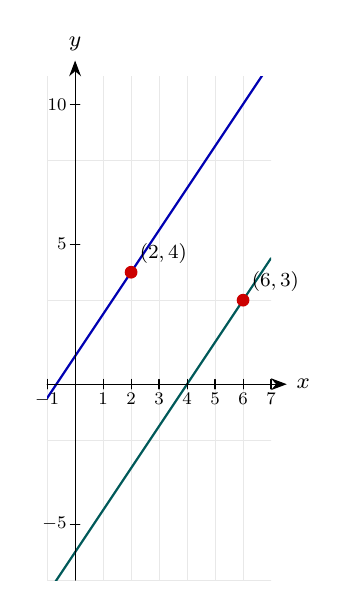
\begin{tikzpicture}[>={Stealth[length=2mm]},font=\footnotesize,line cap=round]
\begin{scope}
\clip (0,0) rectangle (2.844,6.4);
\draw[gray!18] (0,-1.067) grid[xstep=0.356,ystep=1.778] (2.844,6.4);
\draw[blue!70!black,thick] (0,2.311) -- (2.844,6.578);
\draw[teal!70!black,thick] (0,-0.178) -- (2.844,4.089);
\end{scope}
\draw[->] (0,2.489) -- (3.044,2.489) node[right]{$x$};
\draw[->] (0.356,0) -- (0.356,6.6) node[above]{$y$};
\draw (0,2.429) -- (0,2.549) node[below=2pt,scale=0.8]{$-1$};
\draw (0.711,2.429) -- (0.711,2.549) node[below=2pt,scale=0.8]{$1$};
\draw (1.067,2.429) -- (1.067,2.549) node[below=2pt,scale=0.8]{$2$};
\draw (1.422,2.429) -- (1.422,2.549) node[below=2pt,scale=0.8]{$3$};
\draw (1.778,2.429) -- (1.778,2.549) node[below=2pt,scale=0.8]{$4$};
\draw (2.133,2.429) -- (2.133,2.549) node[below=2pt,scale=0.8]{$5$};
\draw (2.489,2.429) -- (2.489,2.549) node[below=2pt,scale=0.8]{$6$};
\draw (2.844,2.429) -- (2.844,2.549) node[below=2pt,scale=0.8]{$7$};
\draw (0.296,0.711) -- (0.416,0.711) node[left=2pt,scale=0.8]{$-5$};
\draw (0.296,4.267) -- (0.416,4.267) node[left=2pt,scale=0.8]{$5$};
\draw (0.296,6.044) -- (0.416,6.044) node[left=2pt,scale=0.8]{$10$};
\fill[red!80!black] (1.067,3.911) circle (2.3pt);
\node[above right,scale=0.9] at (1.067,3.911) {$(2,4)$};
\fill[red!80!black] (2.489,3.556) circle (2.3pt);
\node[above right,scale=0.9] at (2.489,3.556) {$(6,3)$};
\end{tikzpicture}
}
\end{center}
\small The line(s) and key points shown on the coordinate plane.\normalsize

\medskip\hrule

\section*{Parallel and Perpendicular Lines 13\quad\small\texttt{(cg3-013)}}
\addcontentsline{toc}{section}{Parallel and Perpendicular Lines 13 (cg3-013)}
\textit{Difficulty: Foundation \quad\textbar\quad Marks: 3}

\question{Find the equation of the line perpendicular to \( y = 2x - 1 \) that passes through \( (4, 3) \). Give your answer in the form \( y = mx + c \).}

\textbf{Worked solution.}

\textit{Step 1: The gradient of \( y = 2x - 1 \) is \( 2 \). The perpendicular gradient is \( -\dfrac{1}{2} \).}
\[\begin{gathered}
m_\perp = -\dfrac{1}{2}
\end{gathered}\]
Perpendicular gradients multiply to \( -1 \).

\textit{Step 2: Substitute \( (4, 3) \) into \( y = -\frac{1}{2}x + c \).}
\[\begin{gathered}
3 = -\dfrac{1}{2}(4) + c \implies c = 5
\end{gathered}\]
\( -\tfrac{1}{2} \times 4 = -2 \), so \( c = 3 + 2 = 5 \).

\textit{Step 3: Write the equation.}
\[\begin{gathered}
y = -\dfrac{1}{2}x + 5
\end{gathered}\]
Put the gradient and \( y \)-intercept together.

\begin{answerbox}
\textbf{Final answer:}\quad \(\displaystyle y = -\dfrac{1}{2}x + 5\)
\end{answerbox}
\textbf{Diagram.}

\begin{center}
\resizebox{\ifdim\width>\linewidth \linewidth\else \width\fi}{!}{%
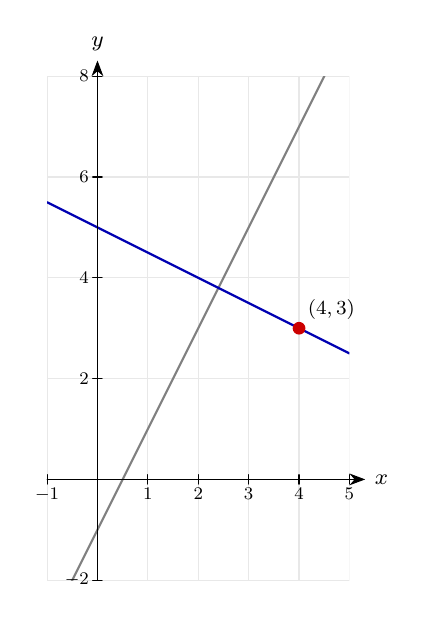
\begin{tikzpicture}[>={Stealth[length=2mm]},font=\footnotesize,line cap=round]
\begin{scope}
\clip (0,0) rectangle (3.84,6.4);
\draw[gray!18] (0,0) grid[xstep=0.64,ystep=1.28] (3.84,6.4);
\draw[gray,thick] (0,-0.64) -- (3.84,7.04);
\draw[blue!70!black,thick] (0,4.8) -- (3.84,2.88);
\end{scope}
\draw[->] (0,1.28) -- (4.04,1.28) node[right]{$x$};
\draw[->] (0.64,0) -- (0.64,6.6) node[above]{$y$};
\draw (0,1.22) -- (0,1.34) node[below=2pt,scale=0.8]{$-1$};
\draw (1.28,1.22) -- (1.28,1.34) node[below=2pt,scale=0.8]{$1$};
\draw (1.92,1.22) -- (1.92,1.34) node[below=2pt,scale=0.8]{$2$};
\draw (2.56,1.22) -- (2.56,1.34) node[below=2pt,scale=0.8]{$3$};
\draw (3.2,1.22) -- (3.2,1.34) node[below=2pt,scale=0.8]{$4$};
\draw (3.84,1.22) -- (3.84,1.34) node[below=2pt,scale=0.8]{$5$};
\draw (0.58,0) -- (0.7,0) node[left=2pt,scale=0.8]{$-2$};
\draw (0.58,2.56) -- (0.7,2.56) node[left=2pt,scale=0.8]{$2$};
\draw (0.58,3.84) -- (0.7,3.84) node[left=2pt,scale=0.8]{$4$};
\draw (0.58,5.12) -- (0.7,5.12) node[left=2pt,scale=0.8]{$6$};
\draw (0.58,6.4) -- (0.7,6.4) node[left=2pt,scale=0.8]{$8$};
\fill[red!80!black] (3.2,3.2) circle (2.3pt);
\node[above right,scale=0.9] at (3.2,3.2) {$(4,3)$};
\end{tikzpicture}
}
\end{center}
\small The line(s) and key points shown on the coordinate plane.\normalsize

\medskip\hrule

\section*{Parallel and Perpendicular Lines 14\quad\small\texttt{(cg3-014)}}
\addcontentsline{toc}{section}{Parallel and Perpendicular Lines 14 (cg3-014)}
\textit{Difficulty: Foundation \quad\textbar\quad Marks: 3}

\question{Find the equation of the line perpendicular to \( y = -\dfrac{1}{3}x + 4 \) that passes through \( (1, -2) \). Give your answer in the form \( y = mx + c \).}

\textbf{Worked solution.}

\textit{Step 1: The given gradient is \( -\frac{1}{3} \). Perpendicular gradient is \( 3 \).}
\[\begin{gathered}
m_\perp = -1 \div \left(-\dfrac{1}{3}\right) = 3
\end{gathered}\]
The perpendicular gradient is the negative reciprocal. Dividing \( -1 \) by a negative gives a positive --- flipping the fraction \( -\tfrac{1}{3} \) and changing sign gives \( +3 \).

\textit{Step 2: Substitute \( (1, -2) \) into \( y = 3x + c \).}
\[\begin{gathered}
-2 = 3(1) + c \implies c = -5
\end{gathered}\]
Substitute the given point. \( c = -2 - 3 = -5 \).

\textit{Step 3: Write the equation.}
\[\begin{gathered}
y = 3x - 5
\end{gathered}\]
Combine gradient and intercept.

\begin{answerbox}
\textbf{Final answer:}\quad \(\displaystyle y = 3x - 5\)
\end{answerbox}
\textbf{Diagram.}

\begin{center}
\resizebox{\ifdim\width>\linewidth \linewidth\else \width\fi}{!}{%
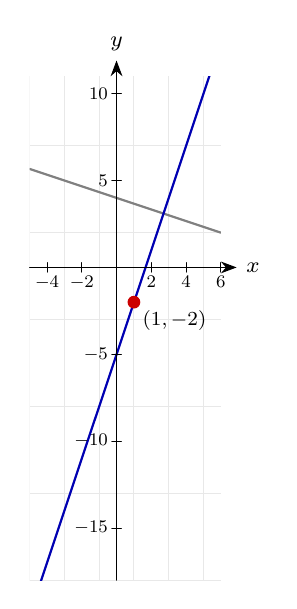
\begin{tikzpicture}[>={Stealth[length=2mm]},font=\footnotesize,line cap=round]
\begin{scope}
\clip (0,0) rectangle (2.428,6.4);
\draw[gray!18] (-0.221,-0.441) grid[xstep=0.441,ystep=1.103] (2.428,6.4);
\draw[gray,thick] (0,5.223) -- (2.428,4.414);
\draw[blue!70!black,thick] (0,-0.441) -- (2.428,6.841);
\end{scope}
\draw[->] (0,3.972) -- (2.628,3.972) node[right]{$x$};
\draw[->] (1.103,0) -- (1.103,6.6) node[above]{$y$};
\draw (0.221,3.912) -- (0.221,4.032) node[below=2pt,scale=0.8]{$-4$};
\draw (0.662,3.912) -- (0.662,4.032) node[below=2pt,scale=0.8]{$-2$};
\draw (1.545,3.912) -- (1.545,4.032) node[below=2pt,scale=0.8]{$2$};
\draw (1.986,3.912) -- (1.986,4.032) node[below=2pt,scale=0.8]{$4$};
\draw (2.428,3.912) -- (2.428,4.032) node[below=2pt,scale=0.8]{$6$};
\draw (1.043,0.662) -- (1.163,0.662) node[left=2pt,scale=0.8]{$-15$};
\draw (1.043,1.766) -- (1.163,1.766) node[left=2pt,scale=0.8]{$-10$};
\draw (1.043,2.869) -- (1.163,2.869) node[left=2pt,scale=0.8]{$-5$};
\draw (1.043,5.076) -- (1.163,5.076) node[left=2pt,scale=0.8]{$5$};
\draw (1.043,6.179) -- (1.163,6.179) node[left=2pt,scale=0.8]{$10$};
\fill[red!80!black] (1.324,3.531) circle (2.3pt);
\node[below right,scale=0.9] at (1.324,3.531) {$(1,-2)$};
\end{tikzpicture}
}
\end{center}
\small The line(s) and key points shown on the coordinate plane.\normalsize

\medskip\hrule

\section*{Parallel and Perpendicular Lines 15\quad\small\texttt{(cg3-015)}}
\addcontentsline{toc}{section}{Parallel and Perpendicular Lines 15 (cg3-015)}
\textit{Difficulty: Foundation \quad\textbar\quad Marks: 4}

\question{Find the equation of the line perpendicular to \( 4x - y + 3 = 0 \) that passes through \( (8, 1) \). Give your answer in the form \( ax + by + c = 0 \).}

\textbf{Worked solution.}

\textit{Step 1: Rearrange \( 4x - y + 3 = 0 \): \( y = 4x + 3 \), so \( m = 4 \).}
\[\begin{gathered}
m_\perp = -\dfrac{1}{4}
\end{gathered}\]
The negative reciprocal of \( 4 \) is \( -\tfrac{1}{4} \), which is the gradient of any line perpendicular to the given one.

\textit{Step 2: Substitute \( (8, 1) \) into \( y = -\frac{1}{4}x + c \).}
\[\begin{gathered}
1 = -\dfrac{1}{4}(8) + c \implies 1 = -2 + c \implies c = 3
\end{gathered}\]
\( -\tfrac{1}{4} \times 8 = -2 \), so adding \( 2 \) to both sides gives \( c = 3 \).

\textit{Step 3: Rearrange \( y = -\frac{1}{4}x + 3 \): multiply by 4.}
\[\begin{gathered}
4y = -x + 12 \implies x + 4y - 12 = 0
\end{gathered}\]
Multiplying by \( 4 \) clears the fraction. Bring everything to one side, keeping the \( x \)-coefficient positive.

\begin{answerbox}
\textbf{Final answer:}\quad \(\displaystyle x + 4y - 12 = 0\)
\end{answerbox}
\textbf{Diagram.}

\begin{center}
\resizebox{\ifdim\width>\linewidth \linewidth\else \width\fi}{!}{%
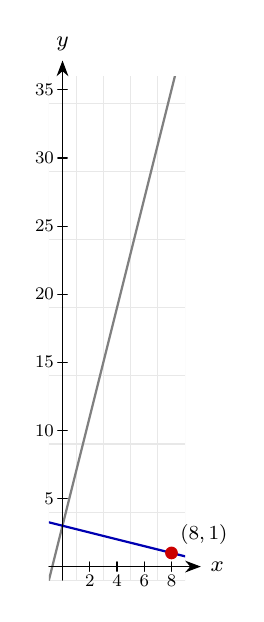
\begin{tikzpicture}[>={Stealth[length=2mm]},font=\footnotesize,line cap=round]
\begin{scope}
\clip (0,0) rectangle (1.73,6.4);
\draw[gray!18] (-0.173,-0.692) grid[xstep=0.346,ystep=0.865] (1.73,6.4);
\draw[gray,thick] (0,0) -- (1.73,6.919);
\draw[blue!70!black,thick] (0,0.735) -- (1.73,0.303);
\end{scope}
\draw[->] (0,0.173) -- (1.93,0.173) node[right]{$x$};
\draw[->] (0.173,0) -- (0.173,6.6) node[above]{$y$};
\draw (0.519,0.113) -- (0.519,0.233) node[below=2pt,scale=0.8]{$2$};
\draw (0.865,0.113) -- (0.865,0.233) node[below=2pt,scale=0.8]{$4$};
\draw (1.211,0.113) -- (1.211,0.233) node[below=2pt,scale=0.8]{$6$};
\draw (1.557,0.113) -- (1.557,0.233) node[below=2pt,scale=0.8]{$8$};
\draw (0.113,1.038) -- (0.233,1.038) node[left=2pt,scale=0.8]{$5$};
\draw (0.113,1.903) -- (0.233,1.903) node[left=2pt,scale=0.8]{$10$};
\draw (0.113,2.768) -- (0.233,2.768) node[left=2pt,scale=0.8]{$15$};
\draw (0.113,3.632) -- (0.233,3.632) node[left=2pt,scale=0.8]{$20$};
\draw (0.113,4.497) -- (0.233,4.497) node[left=2pt,scale=0.8]{$25$};
\draw (0.113,5.362) -- (0.233,5.362) node[left=2pt,scale=0.8]{$30$};
\draw (0.113,6.227) -- (0.233,6.227) node[left=2pt,scale=0.8]{$35$};
\fill[red!80!black] (1.557,0.346) circle (2.3pt);
\node[above right,scale=0.9] at (1.557,0.346) {$(8,1)$};
\end{tikzpicture}
}
\end{center}
\small The line(s) and key points shown on the coordinate plane.\normalsize

\medskip\hrule

\section*{Parallel and Perpendicular Lines 16\quad\small\texttt{(cg3-016)}}
\addcontentsline{toc}{section}{Parallel and Perpendicular Lines 16 (cg3-016)}
\textit{Difficulty: Foundation \quad\textbar\quad Marks: 5}

\question{Find the equation of the line perpendicular to \( 3x + 5y - 2 = 0 \) that passes through \( (-5, 4) \). Give your answer in the form \( ax + by + c = 0 \).}

\textbf{Worked solution.}

\textit{Step 1: Rearrange: \( 5y = -3x + 2 \implies y = -\frac{3}{5}x + \frac{2}{5} \), so \( m = -\frac{3}{5} \).}
\[\begin{gathered}
m_\perp = -1 \div \left(-\dfrac{3}{5}\right) = \dfrac{5}{3}
\end{gathered}\]
Flip the fraction \( -\tfrac{3}{5} \) and change sign to get the perpendicular gradient \( \tfrac{5}{3} \).

\textit{Step 2: Substitute \( (-5, 4) \) into \( y = \frac{5}{3}x + c \).}
\[\begin{gathered}
4 = \dfrac{5}{3}(-5) + c \implies 4 = -\dfrac{25}{3} + c \implies c = \dfrac{37}{3}
\end{gathered}\]
Convert \( 4 \) to thirds: \( 4 = \tfrac{12}{3} \), so \( c = \tfrac{12}{3} + \tfrac{25}{3} = \tfrac{37}{3} \).

\textit{Step 3: Rearrange \( y = \frac{5}{3}x + \frac{37}{3} \): multiply by 3.}
\[\begin{gathered}
3y = 5x + 37 \implies 5x - 3y + 37 = 0
\end{gathered}\]
Multiplying by \( 3 \) clears both fractions in one step. Then rearrange to the required integer form.

\begin{answerbox}
\textbf{Final answer:}\quad \(\displaystyle 5x - 3y + 37 = 0\)
\end{answerbox}
\textbf{Diagram.}

\begin{center}
\resizebox{\ifdim\width>\linewidth \linewidth\else \width\fi}{!}{%
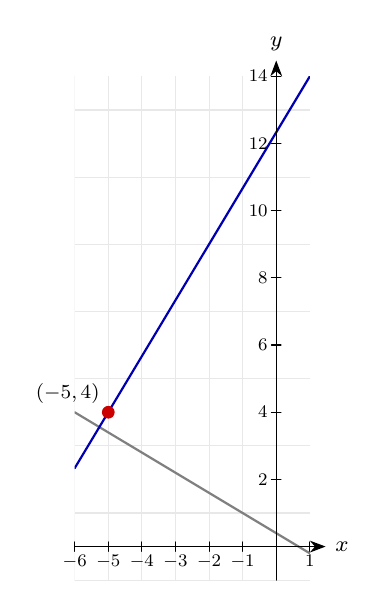
\begin{tikzpicture}[>={Stealth[length=2mm]},font=\footnotesize,line cap=round]
\begin{scope}
\clip (0,0) rectangle (2.987,6.4);
\draw[gray!18] (0,-0.427) grid[xstep=0.427,ystep=0.853] (2.987,6.4);
\draw[gray,thick] (0,2.133) -- (2.987,0.341);
\draw[blue!70!black,thick] (0,1.422) -- (2.987,6.4);
\end{scope}
\draw[->] (0,0.427) -- (3.187,0.427) node[right]{$x$};
\draw[->] (2.56,0) -- (2.56,6.6) node[above]{$y$};
\draw (0,0.367) -- (0,0.487) node[below=2pt,scale=0.8]{$-6$};
\draw (0.427,0.367) -- (0.427,0.487) node[below=2pt,scale=0.8]{$-5$};
\draw (0.853,0.367) -- (0.853,0.487) node[below=2pt,scale=0.8]{$-4$};
\draw (1.28,0.367) -- (1.28,0.487) node[below=2pt,scale=0.8]{$-3$};
\draw (1.707,0.367) -- (1.707,0.487) node[below=2pt,scale=0.8]{$-2$};
\draw (2.133,0.367) -- (2.133,0.487) node[below=2pt,scale=0.8]{$-1$};
\draw (2.987,0.367) -- (2.987,0.487) node[below=2pt,scale=0.8]{$1$};
\draw (2.5,1.28) -- (2.62,1.28) node[left=2pt,scale=0.8]{$2$};
\draw (2.5,2.133) -- (2.62,2.133) node[left=2pt,scale=0.8]{$4$};
\draw (2.5,2.987) -- (2.62,2.987) node[left=2pt,scale=0.8]{$6$};
\draw (2.5,3.84) -- (2.62,3.84) node[left=2pt,scale=0.8]{$8$};
\draw (2.5,4.693) -- (2.62,4.693) node[left=2pt,scale=0.8]{$10$};
\draw (2.5,5.547) -- (2.62,5.547) node[left=2pt,scale=0.8]{$12$};
\draw (2.5,6.4) -- (2.62,6.4) node[left=2pt,scale=0.8]{$14$};
\fill[red!80!black] (0.427,2.133) circle (2.3pt);
\node[above left,scale=0.9] at (0.427,2.133) {$(-5,4)$};
\end{tikzpicture}
}
\end{center}
\small The line(s) and key points shown on the coordinate plane.\normalsize

\medskip\hrule

\section*{Parallel and Perpendicular Lines 17\quad\small\texttt{(cg3-017)}}
\addcontentsline{toc}{section}{Parallel and Perpendicular Lines 17 (cg3-017)}
\textit{Difficulty: Foundation \quad\textbar\quad Marks: 4}

\question{Find the equation of the line perpendicular to \( 2x + 6y - 3 = 0 \) passing through \( (3, -4) \). Give your answer in the form \( y = mx + c \).}

\textbf{Worked solution.}

\textit{Step 1: Rearrange: \( 6y = -2x + 3 \implies m = -\frac{1}{3} \).}
\[\begin{gathered}
m_\perp = 3
\end{gathered}\]
Dividing through by \( 6 \) gives gradient \( -\tfrac{2}{6} = -\tfrac{1}{3} \). The negative reciprocal is \( 3 \).

\textit{Step 2: Substitute \( (3, -4) \) into \( y = 3x + c \).}
\[\begin{gathered}
-4 = 3(3) + c \implies c = -13
\end{gathered}\]
Plug in the point: \( c = -4 - 9 = -13 \).

\textit{Step 3: Write the equation.}
\[\begin{gathered}
y = 3x - 13
\end{gathered}\]
Combine the gradient and \( y \)-intercept.

\begin{answerbox}
\textbf{Final answer:}\quad \(\displaystyle y = 3x - 13\)
\end{answerbox}
\textbf{Diagram.}

\begin{center}
\resizebox{\ifdim\width>\linewidth \linewidth\else \width\fi}{!}{%
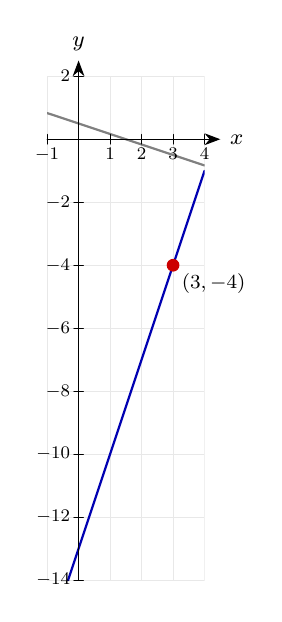
\begin{tikzpicture}[>={Stealth[length=2mm]},font=\footnotesize,line cap=round]
\begin{scope}
\clip (0,0) rectangle (2,6.4);
\draw[gray!18] (0,0) grid[xstep=0.4,ystep=0.8] (2,6.4);
\draw[gray,thick] (0,5.933) -- (2,5.267);
\draw[blue!70!black,thick] (0,-0.8) -- (2,5.2);
\end{scope}
\draw[->] (0,5.6) -- (2.2,5.6) node[right]{$x$};
\draw[->] (0.4,0) -- (0.4,6.6) node[above]{$y$};
\draw (0,5.54) -- (0,5.66) node[below=2pt,scale=0.8]{$-1$};
\draw (0.8,5.54) -- (0.8,5.66) node[below=2pt,scale=0.8]{$1$};
\draw (1.2,5.54) -- (1.2,5.66) node[below=2pt,scale=0.8]{$2$};
\draw (1.6,5.54) -- (1.6,5.66) node[below=2pt,scale=0.8]{$3$};
\draw (2,5.54) -- (2,5.66) node[below=2pt,scale=0.8]{$4$};
\draw (0.34,0) -- (0.46,0) node[left=2pt,scale=0.8]{$-14$};
\draw (0.34,0.8) -- (0.46,0.8) node[left=2pt,scale=0.8]{$-12$};
\draw (0.34,1.6) -- (0.46,1.6) node[left=2pt,scale=0.8]{$-10$};
\draw (0.34,2.4) -- (0.46,2.4) node[left=2pt,scale=0.8]{$-8$};
\draw (0.34,3.2) -- (0.46,3.2) node[left=2pt,scale=0.8]{$-6$};
\draw (0.34,4) -- (0.46,4) node[left=2pt,scale=0.8]{$-4$};
\draw (0.34,4.8) -- (0.46,4.8) node[left=2pt,scale=0.8]{$-2$};
\draw (0.34,6.4) -- (0.46,6.4) node[left=2pt,scale=0.8]{$2$};
\fill[red!80!black] (1.6,4) circle (2.3pt);
\node[below right,scale=0.9] at (1.6,4) {$(3,-4)$};
\end{tikzpicture}
}
\end{center}
\small The line(s) and key points shown on the coordinate plane.\normalsize

\medskip\hrule

\section*{Parallel and Perpendicular Lines 18\quad\small\texttt{(cg3-018)}}
\addcontentsline{toc}{section}{Parallel and Perpendicular Lines 18 (cg3-018)}
\textit{Difficulty: Foundation \quad\textbar\quad Marks: 5}

\question{Line \( M \) is perpendicular to the line joining \( A(1, 5) \) and \( B(4, 11) \), and passes through the midpoint of \( AB \). Find the equation of \( M \) in the form \( y = mx + c \).}

\textbf{Worked solution.}

\textit{Step 1: Find the gradient of \( AB \).}
\[\begin{gathered}
m_{AB} = \dfrac{11 - 5}{4 - 1} = \dfrac{6}{3} = 2
\end{gathered}\]
Apply the gradient formula \( m = \frac{y_2 - y_1}{x_2 - x_1} \) to the two given points.

\textit{Step 2: The perpendicular gradient is \( m_\perp = -\frac{1}{2} \).}
\[\begin{gathered}
m_\perp = -\dfrac{1}{2}
\end{gathered}\]
Negative reciprocal of \( 2 \).

\textit{Step 3: Find the midpoint of \( AB \).}
\[\begin{gathered}
M = \left(\dfrac{1+4}{2},\ \dfrac{5+11}{2}\right) = (2.5,\ 8)
\end{gathered}\]
The midpoint is the average of the endpoint coordinates. \( M \) must pass through this point.

\textit{Step 4: Substitute \( (2.5, 8) \) into \( y = -\frac{1}{2}x + c \).}
\[\begin{gathered}
8 = -\dfrac{1}{2}(2.5) + c \implies c = 9.25
\end{gathered}\]
\( -\tfrac{1}{2} \times 2.5 = -1.25 \), so \( c = 8 + 1.25 = 9.25 \).

\textit{Step 5: Write the equation.}
\[\begin{gathered}
y = -\dfrac{1}{2}x + \dfrac{37}{4}
\end{gathered}\]
\( 9.25 = \frac{37}{4} \).

\begin{answerbox}
\textbf{Final answer:}\quad \(\displaystyle y = -\dfrac{1}{2}x + \dfrac{37}{4}\)
\end{answerbox}
\textbf{Diagram.}

\begin{center}
\resizebox{\ifdim\width>\linewidth \linewidth\else \width\fi}{!}{%
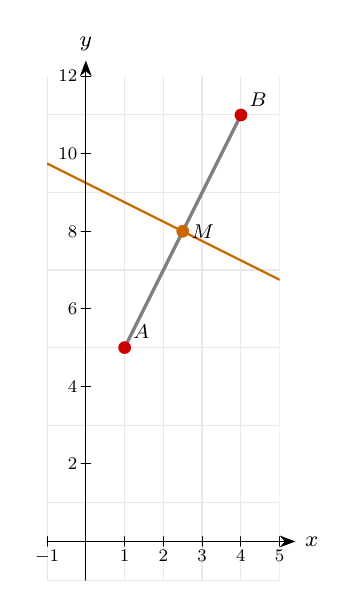
\begin{tikzpicture}[>={Stealth[length=2mm]},font=\footnotesize,line cap=round]
\begin{scope}
\clip (0,0) rectangle (2.954,6.4);
\draw[gray!18] (0,-0.492) grid[xstep=0.492,ystep=0.985] (2.954,6.4);
\draw[orange!80!black,thick] (0,5.292) -- (2.954,3.815);
\draw[gray,very thick] (0.985,2.954) -- (2.462,5.908);
\end{scope}
\draw[->] (0,0.492) -- (3.154,0.492) node[right]{$x$};
\draw[->] (0.492,0) -- (0.492,6.6) node[above]{$y$};
\draw (0,0.432) -- (0,0.552) node[below=2pt,scale=0.8]{$-1$};
\draw (0.985,0.432) -- (0.985,0.552) node[below=2pt,scale=0.8]{$1$};
\draw (1.477,0.432) -- (1.477,0.552) node[below=2pt,scale=0.8]{$2$};
\draw (1.969,0.432) -- (1.969,0.552) node[below=2pt,scale=0.8]{$3$};
\draw (2.462,0.432) -- (2.462,0.552) node[below=2pt,scale=0.8]{$4$};
\draw (2.954,0.432) -- (2.954,0.552) node[below=2pt,scale=0.8]{$5$};
\draw (0.432,1.477) -- (0.552,1.477) node[left=2pt,scale=0.8]{$2$};
\draw (0.432,2.462) -- (0.552,2.462) node[left=2pt,scale=0.8]{$4$};
\draw (0.432,3.446) -- (0.552,3.446) node[left=2pt,scale=0.8]{$6$};
\draw (0.432,4.431) -- (0.552,4.431) node[left=2pt,scale=0.8]{$8$};
\draw (0.432,5.415) -- (0.552,5.415) node[left=2pt,scale=0.8]{$10$};
\draw (0.432,6.4) -- (0.552,6.4) node[left=2pt,scale=0.8]{$12$};
\fill[red!80!black] (0.985,2.954) circle (2.3pt);
\node[above right,scale=0.9] at (0.985,2.954) {$A$};
\fill[red!80!black] (2.462,5.908) circle (2.3pt);
\node[above right,scale=0.9] at (2.462,5.908) {$B$};
\fill[orange!80!black] (1.723,4.431) circle (2.3pt);
\node[right,scale=0.9] at (1.723,4.431) {$M$};
\end{tikzpicture}
}
\end{center}
\small The line(s) and key points shown on the coordinate plane.\normalsize

\medskip\hrule

\section*{Parallel and Perpendicular Lines 19\quad\small\texttt{(cg3-019)}}
\addcontentsline{toc}{section}{Parallel and Perpendicular Lines 19 (cg3-019)}
\textit{Difficulty: Foundation \quad\textbar\quad Marks: 3}

\question{Find the value of \( k \) such that the line \( kx - 2y + 5 = 0 \) is perpendicular to \( y = 4x - 1 \).}

\textbf{Worked solution.}

\textit{Step 1: Rearrange \( kx - 2y + 5 = 0 \): \( y = \frac{k}{2}x + \frac{5}{2} \), gradient \( = \frac{k}{2} \).}
\[\begin{gathered}
m_1 = \dfrac{k}{2}
\end{gathered}\]
Move \( kx + 5 \) across (sign flips), then divide by \( 2 \). Coefficient of \( x \) is the gradient.

\textit{Step 2: For perpendicularity: \( \frac{k}{2} \times 4 = -1 \).}
\[\begin{gathered}
2k = -1 \implies k = -\dfrac{1}{2}
\end{gathered}\]
Multiplying the gradients gives \( \tfrac{4k}{2} = 2k \). Setting this equal to \( -1 \) and dividing by \( 2 \) gives \( k = -\tfrac{1}{2} \).

\begin{answerbox}
\textbf{Final answer:}\quad \(\displaystyle k = -\dfrac{1}{2}\)
\end{answerbox}
\textbf{Diagram.}

\begin{center}
\resizebox{\ifdim\width>\linewidth \linewidth\else \width\fi}{!}{%
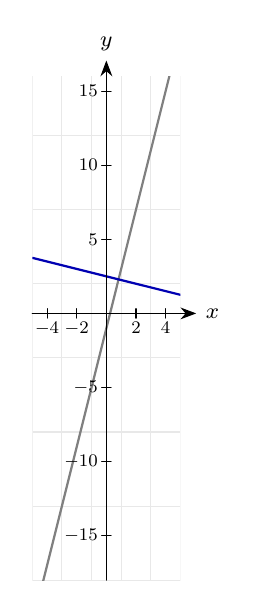
\begin{tikzpicture}[>={Stealth[length=2mm]},font=\footnotesize,line cap=round]
\begin{scope}
\clip (0,0) rectangle (1.882,6.4);
\draw[gray!18] (-0.188,-0.376) grid[xstep=0.376,ystep=0.941] (1.882,6.4);
\draw[gray,thick] (0,-0.565) -- (1.882,6.965);
\draw[blue!70!black,thick] (0,4.094) -- (1.882,3.624);
\end{scope}
\draw[->] (0,3.388) -- (2.082,3.388) node[right]{$x$};
\draw[->] (0.941,0) -- (0.941,6.6) node[above]{$y$};
\draw (0.188,3.328) -- (0.188,3.448) node[below=2pt,scale=0.8]{$-4$};
\draw (0.565,3.328) -- (0.565,3.448) node[below=2pt,scale=0.8]{$-2$};
\draw (1.318,3.328) -- (1.318,3.448) node[below=2pt,scale=0.8]{$2$};
\draw (1.694,3.328) -- (1.694,3.448) node[below=2pt,scale=0.8]{$4$};
\draw (0.881,0.565) -- (1.001,0.565) node[left=2pt,scale=0.8]{$-15$};
\draw (0.881,1.506) -- (1.001,1.506) node[left=2pt,scale=0.8]{$-10$};
\draw (0.881,2.447) -- (1.001,2.447) node[left=2pt,scale=0.8]{$-5$};
\draw (0.881,4.329) -- (1.001,4.329) node[left=2pt,scale=0.8]{$5$};
\draw (0.881,5.271) -- (1.001,5.271) node[left=2pt,scale=0.8]{$10$};
\draw (0.881,6.212) -- (1.001,6.212) node[left=2pt,scale=0.8]{$15$};
\end{tikzpicture}
}
\end{center}
\small The line(s) and key points shown on the coordinate plane.\normalsize

\medskip\hrule

\section*{Parallel and Perpendicular Lines 20\quad\small\texttt{(cg3-020)}}
\addcontentsline{toc}{section}{Parallel and Perpendicular Lines 20 (cg3-020)}
\textit{Difficulty: Foundation \quad\textbar\quad Marks: 5}

\question{Find the equation of the line that is perpendicular to \( 6x - 4y + 1 = 0 \) and passes through the point \( (3, 7) \). Give your answer in the form \( ax + by + c = 0 \).}

\textbf{Worked solution.}

\textit{Step 1: Rearrange: \( 4y = 6x + 1 \implies y = \frac{3}{2}x + \frac{1}{4} \), so \( m = \frac{3}{2} \).}
\[\begin{gathered}
m_\perp = -\dfrac{2}{3}
\end{gathered}\]
Negative reciprocal of \( \tfrac{3}{2} \): flip to \( \tfrac{2}{3} \), change sign.

\textit{Step 2: Substitute \( (3, 7) \) into \( y = -\frac{2}{3}x + c \).}
\[\begin{gathered}
7 = -\dfrac{2}{3}(3) + c \implies c = 9
\end{gathered}\]
\( -\tfrac{2}{3} \times 3 = -2 \), so \( c = 7 + 2 = 9 \).

\textit{Step 3: Rearrange \( y = -\frac{2}{3}x + 9 \): multiply by 3.}
\[\begin{gathered}
3y = -2x + 27 \implies 2x + 3y - 27 = 0
\end{gathered}\]
Multiplying by \( 3 \) clears the fraction; then collect all terms on one side.

\begin{answerbox}
\textbf{Final answer:}\quad \(\displaystyle 2x + 3y - 27 = 0\)
\end{answerbox}
\textbf{Diagram.}

\begin{center}
\resizebox{\ifdim\width>\linewidth \linewidth\else \width\fi}{!}{%
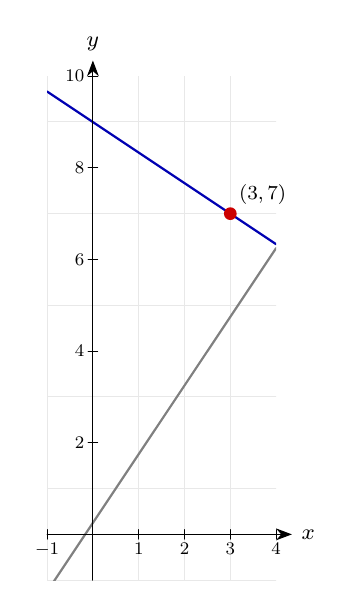
\begin{tikzpicture}[>={Stealth[length=2mm]},font=\footnotesize,line cap=round]
\begin{scope}
\clip (0,0) rectangle (2.909,6.4);
\draw[gray!18] (0,-0.582) grid[xstep=0.582,ystep=1.164] (2.909,6.4);
\draw[gray,thick] (0,-0.145) -- (2.909,4.218);
\draw[blue!70!black,thick] (0,6.206) -- (2.909,4.267);
\end{scope}
\draw[->] (0,0.582) -- (3.109,0.582) node[right]{$x$};
\draw[->] (0.582,0) -- (0.582,6.6) node[above]{$y$};
\draw (0,0.522) -- (0,0.642) node[below=2pt,scale=0.8]{$-1$};
\draw (1.164,0.522) -- (1.164,0.642) node[below=2pt,scale=0.8]{$1$};
\draw (1.745,0.522) -- (1.745,0.642) node[below=2pt,scale=0.8]{$2$};
\draw (2.327,0.522) -- (2.327,0.642) node[below=2pt,scale=0.8]{$3$};
\draw (2.909,0.522) -- (2.909,0.642) node[below=2pt,scale=0.8]{$4$};
\draw (0.522,1.745) -- (0.642,1.745) node[left=2pt,scale=0.8]{$2$};
\draw (0.522,2.909) -- (0.642,2.909) node[left=2pt,scale=0.8]{$4$};
\draw (0.522,4.073) -- (0.642,4.073) node[left=2pt,scale=0.8]{$6$};
\draw (0.522,5.236) -- (0.642,5.236) node[left=2pt,scale=0.8]{$8$};
\draw (0.522,6.4) -- (0.642,6.4) node[left=2pt,scale=0.8]{$10$};
\fill[red!80!black] (2.327,4.655) circle (2.3pt);
\node[above right,scale=0.9] at (2.327,4.655) {$(3,7)$};
\end{tikzpicture}
}
\end{center}
\small The line(s) and key points shown on the coordinate plane.\normalsize

\medskip\hrule

\section*{Parallel and Perpendicular Lines 21\quad\small\texttt{(cg3-021)}}
\addcontentsline{toc}{section}{Parallel and Perpendicular Lines 21 (cg3-021)}
\textit{Difficulty: Foundation \quad\textbar\quad Marks: 4}

\question{Line \( Q \) passes through \( (a, b) \) and is perpendicular to \( 5x - 2y = 10 \). Find an equation for \( Q \) in terms of \( a \) and \( b \).}

\textbf{Worked solution.}

\textit{Step 1: Rearrange the given line: \( y = \frac{5}{2}x - 5 \), so \( m = \frac{5}{2} \).}
\[\begin{gathered}
m_\perp = -\dfrac{2}{5}
\end{gathered}\]
Negative reciprocal of \( \tfrac{5}{2} \) is \( -\tfrac{2}{5} \).

\textit{Step 2: Use point \( (a, b) \) and gradient \( -\frac{2}{5} \).}
\[\begin{gathered}
y - b = -\dfrac{2}{5}(x - a)
\end{gathered}\]
Point-slope form. This is the cleanest starting form when the point is given as algebraic letters rather than numbers.

\textit{Step 3: Multiply through by 5 and rearrange.}
\[\begin{gathered}
5y - 5b = -2x + 2a \implies 2x + 5y = 2a + 5b
\end{gathered}\]
Multiplying by \( 5 \) clears the fraction. Then bring the \( x \)-term to the left to give a tidy form with integer coefficients of \( x \) and \( y \).

\begin{answerbox}
\textbf{Final answer:}\quad \(\displaystyle 2x + 5y = 2a + 5b\)
\end{answerbox}
\textbf{Diagram.}

\begin{center}
\resizebox{\ifdim\width>\linewidth \linewidth\else \width\fi}{!}{%
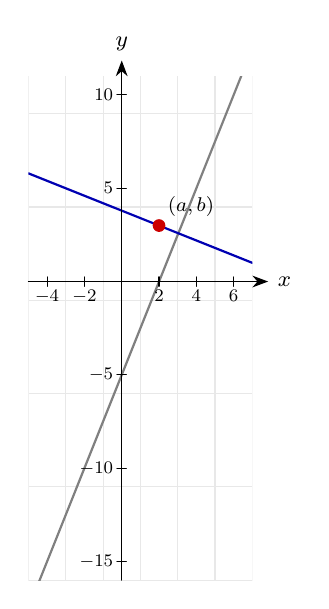
\begin{tikzpicture}[>={Stealth[length=2mm]},font=\footnotesize,line cap=round]
\begin{scope}
\clip (0,0) rectangle (2.844,6.4);
\draw[gray!18] (-0.237,-0.948) grid[xstep=0.474,ystep=1.185] (2.844,6.4);
\draw[gray,thick] (0,-0.356) -- (2.844,6.756);
\draw[blue!70!black,thick] (0,5.167) -- (2.844,4.03);
\end{scope}
\draw[->] (0,3.793) -- (3.044,3.793) node[right]{$x$};
\draw[->] (1.185,0) -- (1.185,6.6) node[above]{$y$};
\draw (0.237,3.733) -- (0.237,3.853) node[below=2pt,scale=0.8]{$-4$};
\draw (0.711,3.733) -- (0.711,3.853) node[below=2pt,scale=0.8]{$-2$};
\draw (1.659,3.733) -- (1.659,3.853) node[below=2pt,scale=0.8]{$2$};
\draw (2.133,3.733) -- (2.133,3.853) node[below=2pt,scale=0.8]{$4$};
\draw (2.607,3.733) -- (2.607,3.853) node[below=2pt,scale=0.8]{$6$};
\draw (1.125,0.237) -- (1.245,0.237) node[left=2pt,scale=0.8]{$-15$};
\draw (1.125,1.422) -- (1.245,1.422) node[left=2pt,scale=0.8]{$-10$};
\draw (1.125,2.607) -- (1.245,2.607) node[left=2pt,scale=0.8]{$-5$};
\draw (1.125,4.978) -- (1.245,4.978) node[left=2pt,scale=0.8]{$5$};
\draw (1.125,6.163) -- (1.245,6.163) node[left=2pt,scale=0.8]{$10$};
\fill[red!80!black] (1.659,4.504) circle (2.3pt);
\node[above right,scale=0.9] at (1.659,4.504) {$(a,b)$};
\end{tikzpicture}
}
\end{center}
\small The line(s) and key points shown on the coordinate plane.\normalsize

\medskip\hrule

\section*{Parallel and Perpendicular Lines 22\quad\small\texttt{(cg3-022)}}
\addcontentsline{toc}{section}{Parallel and Perpendicular Lines 22 (cg3-022)}
\textit{Difficulty: Foundation \quad\textbar\quad Marks: 4}

\question{The line \( L_1 \) has equation \( y = \dfrac{2}{3}x + 1 \). Line \( L_2 \) is perpendicular to \( L_1 \) and intersects the \( x \)-axis at \( x = 6 \). Find the equation of \( L_2 \).}

\textbf{Worked solution.}

\textit{Step 1: The gradient of \( L_2 \) is the negative reciprocal of \( \frac{2}{3} \).}
\[\begin{gathered}
m_\perp = -\dfrac{3}{2}
\end{gathered}\]
Flip the fraction and change sign.

\textit{Step 2: \( L_2 \) passes through \( (6, 0) \) (intersects \( x \)-axis at \( x = 6 \)).}
\[\begin{gathered}
0 = -\dfrac{3}{2}(6) + c \implies c = 9
\end{gathered}\]
On the \( x \)-axis \( y = 0 \). Substitute \( (6, 0) \): \( -\tfrac{3}{2} \times 6 = -9 \), so \( c = 9 \).

\textit{Step 3: Write the equation.}
\[\begin{gathered}
y = -\dfrac{3}{2}x + 9
\end{gathered}\]
Combine the gradient and intercept.

\begin{answerbox}
\textbf{Final answer:}\quad \(\displaystyle y = -\dfrac{3}{2}x + 9\)
\end{answerbox}
\textbf{Diagram.}

\begin{center}
\resizebox{\ifdim\width>\linewidth \linewidth\else \width\fi}{!}{%
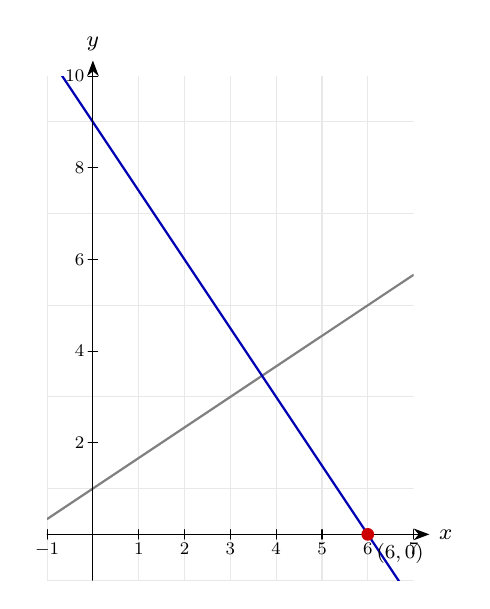
\begin{tikzpicture}[>={Stealth[length=2mm]},font=\footnotesize,line cap=round]
\begin{scope}
\clip (0,0) rectangle (4.655,6.4);
\draw[gray!18] (0,-0.582) grid[xstep=0.582,ystep=1.164] (4.655,6.4);
\draw[gray,thick] (0,0.776) -- (4.655,3.879);
\draw[blue!70!black,thick] (0,6.691) -- (4.655,-0.291);
\end{scope}
\draw[->] (0,0.582) -- (4.855,0.582) node[right]{$x$};
\draw[->] (0.582,0) -- (0.582,6.6) node[above]{$y$};
\draw (0,0.522) -- (0,0.642) node[below=2pt,scale=0.8]{$-1$};
\draw (1.164,0.522) -- (1.164,0.642) node[below=2pt,scale=0.8]{$1$};
\draw (1.745,0.522) -- (1.745,0.642) node[below=2pt,scale=0.8]{$2$};
\draw (2.327,0.522) -- (2.327,0.642) node[below=2pt,scale=0.8]{$3$};
\draw (2.909,0.522) -- (2.909,0.642) node[below=2pt,scale=0.8]{$4$};
\draw (3.491,0.522) -- (3.491,0.642) node[below=2pt,scale=0.8]{$5$};
\draw (4.073,0.522) -- (4.073,0.642) node[below=2pt,scale=0.8]{$6$};
\draw (4.655,0.522) -- (4.655,0.642) node[below=2pt,scale=0.8]{$7$};
\draw (0.522,1.745) -- (0.642,1.745) node[left=2pt,scale=0.8]{$2$};
\draw (0.522,2.909) -- (0.642,2.909) node[left=2pt,scale=0.8]{$4$};
\draw (0.522,4.073) -- (0.642,4.073) node[left=2pt,scale=0.8]{$6$};
\draw (0.522,5.236) -- (0.642,5.236) node[left=2pt,scale=0.8]{$8$};
\draw (0.522,6.4) -- (0.642,6.4) node[left=2pt,scale=0.8]{$10$};
\fill[red!80!black] (4.073,0.582) circle (2.3pt);
\node[below right,scale=0.9] at (4.073,0.582) {$(6,0)$};
\end{tikzpicture}
}
\end{center}
\small The line(s) and key points shown on the coordinate plane.\normalsize

\medskip\hrule

\section*{Parallel and Perpendicular Lines 23\quad\small\texttt{(cg3-023)}}
\addcontentsline{toc}{section}{Parallel and Perpendicular Lines 23 (cg3-023)}
\textit{Difficulty: Foundation \quad\textbar\quad Marks: 5}

\question{Find the equation of the perpendicular bisector of the line segment joining \( A(2, 6) \) and \( B(8, 2) \). Give your answer in the form \( y = mx + c \).}

\textbf{Worked solution.}

\textit{Step 1: Find the midpoint of \( AB \).}
\[\begin{gathered}
M = \left(\dfrac{2+8}{2},\ \dfrac{6+2}{2}\right) = (5,\ 4)
\end{gathered}\]
The perpendicular bisector must pass through the midpoint of \( AB \). Average the coordinates.

\textit{Step 2: Find the gradient of \( AB \).}
\[\begin{gathered}
m_{AB} = \dfrac{2 - 6}{8 - 2} = \dfrac{-4}{6} = -\dfrac{2}{3}
\end{gathered}\]
Apply the gradient formula. Simplify \( -\tfrac{4}{6} \) by cancelling a factor of \( 2 \).

\textit{Step 3: Perpendicular gradient:}
\[\begin{gathered}
m_\perp = \dfrac{3}{2}
\end{gathered}\]
Negative reciprocal of \( -\tfrac{2}{3} \) is \( \tfrac{3}{2} \) (flip and change sign --- two negatives cancel).

\textit{Step 4: Substitute midpoint \( (5, 4) \) into \( y = \frac{3}{2}x + c \).}
\[\begin{gathered}
4 = \dfrac{3}{2}(5) + c \implies c = 4 - \dfrac{15}{2} = -\dfrac{7}{2}
\end{gathered}\]
\( \tfrac{3}{2} \times 5 = \tfrac{15}{2} \). Then \( 4 - \tfrac{15}{2} = \tfrac{8}{2} - \tfrac{15}{2} = -\tfrac{7}{2} \).

\textit{Step 5: Write the equation.}
\[\begin{gathered}
y = \dfrac{3}{2}x - \dfrac{7}{2}
\end{gathered}\]
Combine gradient and \( y \)-intercept.

\begin{answerbox}
\textbf{Final answer:}\quad \(\displaystyle y = \dfrac{3}{2}x - \dfrac{7}{2}\)
\end{answerbox}
\textbf{Diagram.}

\begin{center}
\resizebox{\ifdim\width>\linewidth \linewidth\else \width\fi}{!}{%
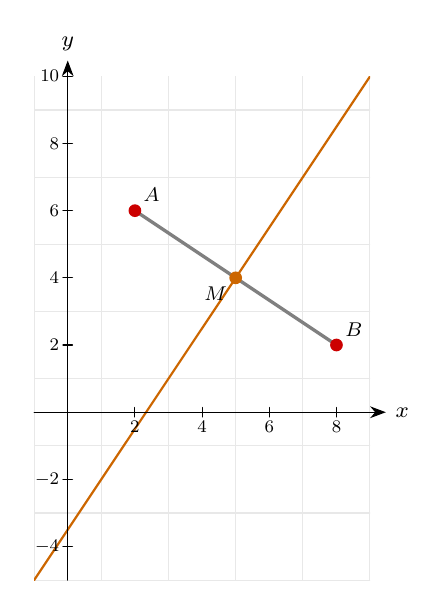
\begin{tikzpicture}[>={Stealth[length=2mm]},font=\footnotesize,line cap=round]
\begin{scope}
\clip (0,0) rectangle (4.267,6.4);
\draw[gray!18] (-0.427,-0.427) grid[xstep=0.853,ystep=0.853] (4.267,6.4);
\draw[orange!80!black,thick] (0,0) -- (4.267,6.4);
\draw[gray,very thick] (1.28,4.693) -- (3.84,2.987);
\end{scope}
\draw[->] (0,2.133) -- (4.467,2.133) node[right]{$x$};
\draw[->] (0.427,0) -- (0.427,6.6) node[above]{$y$};
\draw (1.28,2.073) -- (1.28,2.193) node[below=2pt,scale=0.8]{$2$};
\draw (2.133,2.073) -- (2.133,2.193) node[below=2pt,scale=0.8]{$4$};
\draw (2.987,2.073) -- (2.987,2.193) node[below=2pt,scale=0.8]{$6$};
\draw (3.84,2.073) -- (3.84,2.193) node[below=2pt,scale=0.8]{$8$};
\draw (0.367,0.427) -- (0.487,0.427) node[left=2pt,scale=0.8]{$-4$};
\draw (0.367,1.28) -- (0.487,1.28) node[left=2pt,scale=0.8]{$-2$};
\draw (0.367,2.987) -- (0.487,2.987) node[left=2pt,scale=0.8]{$2$};
\draw (0.367,3.84) -- (0.487,3.84) node[left=2pt,scale=0.8]{$4$};
\draw (0.367,4.693) -- (0.487,4.693) node[left=2pt,scale=0.8]{$6$};
\draw (0.367,5.547) -- (0.487,5.547) node[left=2pt,scale=0.8]{$8$};
\draw (0.367,6.4) -- (0.487,6.4) node[left=2pt,scale=0.8]{$10$};
\fill[red!80!black] (1.28,4.693) circle (2.3pt);
\node[above right,scale=0.9] at (1.28,4.693) {$A$};
\fill[red!80!black] (3.84,2.987) circle (2.3pt);
\node[above right,scale=0.9] at (3.84,2.987) {$B$};
\fill[orange!80!black] (2.56,3.84) circle (2.3pt);
\node[below left,scale=0.9] at (2.56,3.84) {$M$};
\end{tikzpicture}
}
\end{center}
\small The line(s) and key points shown on the coordinate plane.\normalsize

\medskip\hrule

\section*{Parallel and Perpendicular Lines 24\quad\small\texttt{(cg3-024)}}
\addcontentsline{toc}{section}{Parallel and Perpendicular Lines 24 (cg3-024)}
\textit{Difficulty: Foundation \quad\textbar\quad Marks: 5}

\question{Find the equation of the perpendicular bisector of the segment joining \( P(-2, 1) \) and \( Q(4, 7) \). Give your answer in the form \( ax + by + c = 0 \).}

\textbf{Worked solution.}

\textit{Step 1: Midpoint of \( PQ \):}
\[\begin{gathered}
M = \left(\dfrac{-2+4}{2},\ \dfrac{1+7}{2}\right) = (1,\ 4)
\end{gathered}\]
Average the \( x \)- and \( y \)-coordinates. The perpendicular bisector must pass through this point.

\textit{Step 2: Gradient of \( PQ \):}
\[\begin{gathered}
m_{PQ} = \dfrac{7 - 1}{4 - (-2)} = \dfrac{6}{6} = 1
\end{gathered}\]
Watch the double negative: \( 4 - (-2) = 6 \), not \( 2 \).

\textit{Step 3: Perpendicular gradient: \( m_\perp = -1 \).}
\[\begin{gathered}
y = -x + c
\end{gathered}\]
Negative reciprocal of \( 1 \) is \( -1 \).

\textit{Step 4: Substitute \( (1, 4) \).}
\[\begin{gathered}
4 = -1 + c \implies c = 5 \implies y = -x + 5
\end{gathered}\]
Substitute the midpoint to find \( c \): \( c = 4 + 1 = 5 \).

\textit{Step 5: Rearrange.}
\[\begin{gathered}
x + y - 5 = 0
\end{gathered}\]
Add \( x \) and subtract \( 5 \) from both sides to put it in the required form.

\begin{answerbox}
\textbf{Final answer:}\quad \(\displaystyle x + y - 5 = 0\)
\end{answerbox}
\textbf{Diagram.}

\begin{center}
\resizebox{\ifdim\width>\linewidth \linewidth\else \width\fi}{!}{%
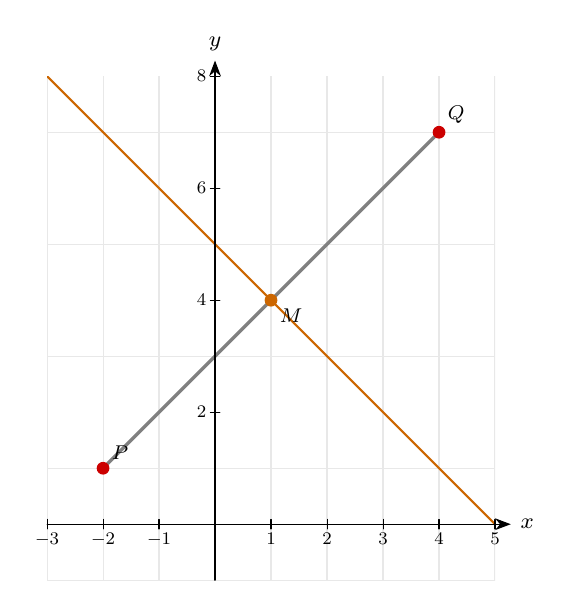
\begin{tikzpicture}[>={Stealth[length=2mm]},font=\footnotesize,line cap=round]
\begin{scope}
\clip (0,0) rectangle (5.689,6.4);
\draw[gray!18] (0,-0.711) grid[xstep=0.711,ystep=1.422] (5.689,6.4);
\draw[orange!80!black,thick] (0,6.4) -- (5.689,0.711);
\draw[gray,very thick] (0.711,1.422) -- (4.978,5.689);
\end{scope}
\draw[->] (0,0.711) -- (5.889,0.711) node[right]{$x$};
\draw[->] (2.133,0) -- (2.133,6.6) node[above]{$y$};
\draw (0,0.651) -- (0,0.771) node[below=2pt,scale=0.8]{$-3$};
\draw (0.711,0.651) -- (0.711,0.771) node[below=2pt,scale=0.8]{$-2$};
\draw (1.422,0.651) -- (1.422,0.771) node[below=2pt,scale=0.8]{$-1$};
\draw (2.844,0.651) -- (2.844,0.771) node[below=2pt,scale=0.8]{$1$};
\draw (3.556,0.651) -- (3.556,0.771) node[below=2pt,scale=0.8]{$2$};
\draw (4.267,0.651) -- (4.267,0.771) node[below=2pt,scale=0.8]{$3$};
\draw (4.978,0.651) -- (4.978,0.771) node[below=2pt,scale=0.8]{$4$};
\draw (5.689,0.651) -- (5.689,0.771) node[below=2pt,scale=0.8]{$5$};
\draw (2.073,2.133) -- (2.193,2.133) node[left=2pt,scale=0.8]{$2$};
\draw (2.073,3.556) -- (2.193,3.556) node[left=2pt,scale=0.8]{$4$};
\draw (2.073,4.978) -- (2.193,4.978) node[left=2pt,scale=0.8]{$6$};
\draw (2.073,6.4) -- (2.193,6.4) node[left=2pt,scale=0.8]{$8$};
\fill[red!80!black] (0.711,1.422) circle (2.3pt);
\node[above right,scale=0.9] at (0.711,1.422) {$P$};
\fill[red!80!black] (4.978,5.689) circle (2.3pt);
\node[above right,scale=0.9] at (4.978,5.689) {$Q$};
\fill[orange!80!black] (2.844,3.556) circle (2.3pt);
\node[below right,scale=0.9] at (2.844,3.556) {$M$};
\end{tikzpicture}
}
\end{center}
\small The line(s) and key points shown on the coordinate plane.\normalsize

\medskip\hrule

\section*{Parallel and Perpendicular Lines 25\quad\small\texttt{(cg3-025)}}
\addcontentsline{toc}{section}{Parallel and Perpendicular Lines 25 (cg3-025)}
\textit{Difficulty: Foundation \quad\textbar\quad Marks: 6}

\question{The perpendicular bisector of segment \( CD \) has equation \( y = 2x - 3 \). If \( C = (1, 4) \), find the coordinates of \( D \).}

\textbf{Worked solution.}

\textit{Step 1: The perpendicular bisector has gradient 2, so \( CD \) has gradient \( -\frac{1}{2} \).}
\[\begin{gathered}
m_{CD} = -\dfrac{1}{2}
\end{gathered}\]
\( CD \) is perpendicular to its bisector, so its gradient is the negative reciprocal of \( 2 \).

\textit{Step 2: The midpoint of \( CD \) lies on \( y = 2x - 3 \). Let midpoint be \( M(h, k) \) with \( k = 2h - 3 \).}
\[\begin{gathered}
k = 2h - 3
\end{gathered}\]
Every perpendicular bisector passes through the midpoint of its segment, so \( M \) lies on the given line.

\textit{Step 3: The gradient from \( C(1,4) \) to \( M(h,k) \) equals \( -\frac{1}{2} \):}
\[\begin{gathered}
\dfrac{k - 4}{h - 1} = -\dfrac{1}{2} \implies 2(k - 4) = -(h - 1)
\end{gathered}\]
Cross-multiplying eliminates the fraction. This second equation lets us pin down \( M \) together with the first one.

\textit{Step 4: Substitute \( k = 2h - 3 \):}
\[\begin{gathered}
2(2h - 3 - 4) = -(h - 1) \implies 2(2h - 7) = -h + 1 \implies 4h - 14 = -h + 1 \implies 5h = 15 \implies h = 3,\ k = 3
\end{gathered}\]
Substitute the line equation into the gradient equation to eliminate \( k \), expand both sides, then solve the linear equation for \( h \). Then \( k = 2(3) - 3 = 3 \). Midpoint \( M = (3, 3) \).

\textit{Step 5: Find \( D \): \( D = 2M - C \).}
\[\begin{gathered}
D = (2(3) - 1,\ 2(3) - 4) = (5,\ 2)
\end{gathered}\]
Since \( M \) is the midpoint of \( CD \), \( M = \tfrac{1}{2}(C + D) \), so \( D = 2M - C \) coordinate-wise.

\begin{answerbox}
\textbf{Final answer:}\quad \(\displaystyle D = (5, 2)\)
\end{answerbox}
\textbf{Diagram.}

\begin{center}
\resizebox{\ifdim\width>\linewidth \linewidth\else \width\fi}{!}{%
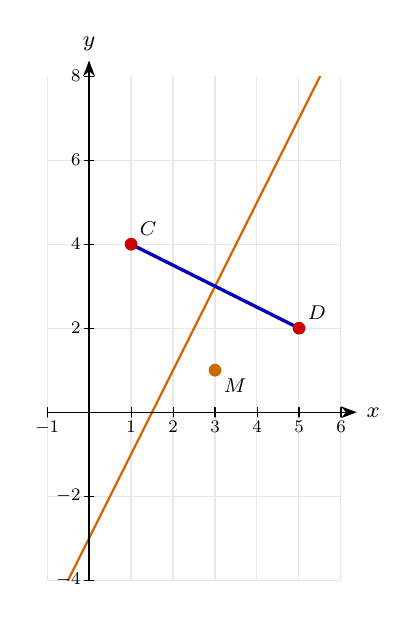
\begin{tikzpicture}[>={Stealth[length=2mm]},font=\footnotesize,line cap=round]
\begin{scope}
\clip (0,0) rectangle (3.733,6.4);
\draw[gray!18] (0,0) grid[xstep=0.533,ystep=1.067] (3.733,6.4);
\draw[orange!80!black,thick] (0,-0.533) -- (3.733,6.933);
\draw[blue!70!black,very thick] (1.067,4.267) -- (3.2,3.2);
\end{scope}
\draw[->] (0,2.133) -- (3.933,2.133) node[right]{$x$};
\draw[->] (0.533,0) -- (0.533,6.6) node[above]{$y$};
\draw (0,2.073) -- (0,2.193) node[below=2pt,scale=0.8]{$-1$};
\draw (1.067,2.073) -- (1.067,2.193) node[below=2pt,scale=0.8]{$1$};
\draw (1.6,2.073) -- (1.6,2.193) node[below=2pt,scale=0.8]{$2$};
\draw (2.133,2.073) -- (2.133,2.193) node[below=2pt,scale=0.8]{$3$};
\draw (2.667,2.073) -- (2.667,2.193) node[below=2pt,scale=0.8]{$4$};
\draw (3.2,2.073) -- (3.2,2.193) node[below=2pt,scale=0.8]{$5$};
\draw (3.733,2.073) -- (3.733,2.193) node[below=2pt,scale=0.8]{$6$};
\draw (0.473,0) -- (0.593,0) node[left=2pt,scale=0.8]{$-4$};
\draw (0.473,1.067) -- (0.593,1.067) node[left=2pt,scale=0.8]{$-2$};
\draw (0.473,3.2) -- (0.593,3.2) node[left=2pt,scale=0.8]{$2$};
\draw (0.473,4.267) -- (0.593,4.267) node[left=2pt,scale=0.8]{$4$};
\draw (0.473,5.333) -- (0.593,5.333) node[left=2pt,scale=0.8]{$6$};
\draw (0.473,6.4) -- (0.593,6.4) node[left=2pt,scale=0.8]{$8$};
\fill[red!80!black] (1.067,4.267) circle (2.3pt);
\node[above right,scale=0.9] at (1.067,4.267) {$C$};
\fill[red!80!black] (3.2,3.2) circle (2.3pt);
\node[above right,scale=0.9] at (3.2,3.2) {$D$};
\fill[orange!80!black] (2.133,2.667) circle (2.3pt);
\node[below right,scale=0.9] at (2.133,2.667) {$M$};
\end{tikzpicture}
}
\end{center}
\small The line(s) and key points shown on the coordinate plane.\normalsize

\medskip\hrule

\section*{Parallel and Perpendicular Lines 26\quad\small\texttt{(cg3-026)}}
\addcontentsline{toc}{section}{Parallel and Perpendicular Lines 26 (cg3-026)}
\textit{Difficulty: Foundation \quad\textbar\quad Marks: 5}

\question{Find the equation of the perpendicular bisector of the segment joining \( A(0, -3) \) and \( B(6, 5) \). Give your answer in the form \( ax + by + c = 0 \).}

\textbf{Worked solution.}

\textit{Step 1: Midpoint:}
\[\begin{gathered}
M = \left(3,\ 1\right)
\end{gathered}\]
Averaging coordinates: \( \tfrac{0+6}{2} = 3 \) and \( \tfrac{-3+5}{2} = 1 \).

\textit{Step 2: Gradient of \( AB \):}
\[\begin{gathered}
m_{AB} = \dfrac{5-(-3)}{6-0} = \dfrac{8}{6} = \dfrac{4}{3}
\end{gathered}\]
Watch the double negative: \( 5 - (-3) = 8 \). Then simplify \( \tfrac{8}{6} \) by cancelling a factor of \( 2 \).

\textit{Step 3: Perpendicular gradient:}
\[\begin{gathered}
m_\perp = -\dfrac{3}{4}
\end{gathered}\]
Negative reciprocal of \( \tfrac{4}{3} \): flip the fraction and change sign.

\textit{Step 4: Substitute \( M(3,1) \) into \( y = -\frac{3}{4}x + c \):}
\[\begin{gathered}
1 = -\dfrac{9}{4} + c \implies c = \dfrac{13}{4}
\end{gathered}\]
\( -\tfrac{3}{4} \times 3 = -\tfrac{9}{4} \). Then \( c = 1 + \tfrac{9}{4} = \tfrac{4}{4} + \tfrac{9}{4} = \tfrac{13}{4} \).

\textit{Step 5: Multiply through by 4 and rearrange:}
\[\begin{gathered}
4y = -3x + 13 \implies 3x + 4y - 13 = 0
\end{gathered}\]
Multiplying by \( 4 \) clears both fractions in one stroke. Then move \( -3x + 13 \) to the left.

\begin{answerbox}
\textbf{Final answer:}\quad \(\displaystyle 3x + 4y - 13 = 0\)
\end{answerbox}
\textbf{Diagram.}

\begin{center}
\resizebox{\ifdim\width>\linewidth \linewidth\else \width\fi}{!}{%
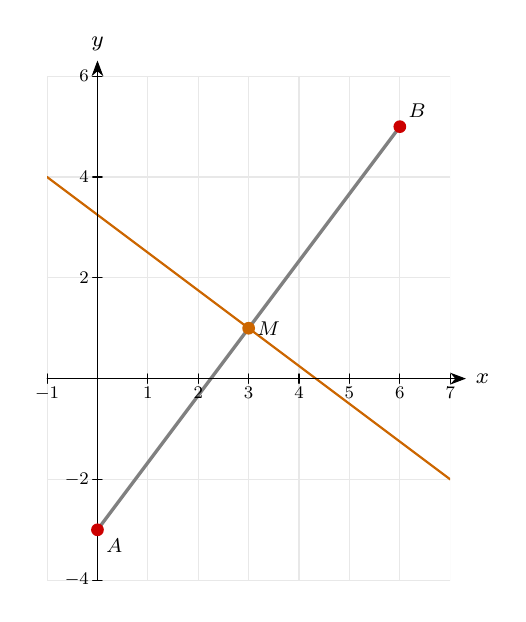
\begin{tikzpicture}[>={Stealth[length=2mm]},font=\footnotesize,line cap=round]
\begin{scope}
\clip (0,0) rectangle (5.12,6.4);
\draw[gray!18] (0,0) grid[xstep=0.64,ystep=1.28] (5.12,6.4);
\draw[orange!80!black,thick] (0,5.12) -- (5.12,1.28);
\draw[gray,very thick] (0.64,0.64) -- (4.48,5.76);
\end{scope}
\draw[->] (0,2.56) -- (5.32,2.56) node[right]{$x$};
\draw[->] (0.64,0) -- (0.64,6.6) node[above]{$y$};
\draw (0,2.5) -- (0,2.62) node[below=2pt,scale=0.8]{$-1$};
\draw (1.28,2.5) -- (1.28,2.62) node[below=2pt,scale=0.8]{$1$};
\draw (1.92,2.5) -- (1.92,2.62) node[below=2pt,scale=0.8]{$2$};
\draw (2.56,2.5) -- (2.56,2.62) node[below=2pt,scale=0.8]{$3$};
\draw (3.2,2.5) -- (3.2,2.62) node[below=2pt,scale=0.8]{$4$};
\draw (3.84,2.5) -- (3.84,2.62) node[below=2pt,scale=0.8]{$5$};
\draw (4.48,2.5) -- (4.48,2.62) node[below=2pt,scale=0.8]{$6$};
\draw (5.12,2.5) -- (5.12,2.62) node[below=2pt,scale=0.8]{$7$};
\draw (0.58,0) -- (0.7,0) node[left=2pt,scale=0.8]{$-4$};
\draw (0.58,1.28) -- (0.7,1.28) node[left=2pt,scale=0.8]{$-2$};
\draw (0.58,3.84) -- (0.7,3.84) node[left=2pt,scale=0.8]{$2$};
\draw (0.58,5.12) -- (0.7,5.12) node[left=2pt,scale=0.8]{$4$};
\draw (0.58,6.4) -- (0.7,6.4) node[left=2pt,scale=0.8]{$6$};
\fill[red!80!black] (0.64,0.64) circle (2.3pt);
\node[below right,scale=0.9] at (0.64,0.64) {$A$};
\fill[red!80!black] (4.48,5.76) circle (2.3pt);
\node[above right,scale=0.9] at (4.48,5.76) {$B$};
\fill[orange!80!black] (2.56,3.2) circle (2.3pt);
\node[right,scale=0.9] at (2.56,3.2) {$M$};
\end{tikzpicture}
}
\end{center}
\small The line(s) and key points shown on the coordinate plane.\normalsize

\medskip\hrule

\section*{Parallel and Perpendicular Lines 27\quad\small\texttt{(cg3-027)}}
\addcontentsline{toc}{section}{Parallel and Perpendicular Lines 27 (cg3-027)}
\textit{Difficulty: Foundation \quad\textbar\quad Marks: 7}

\question{Triangle \( PQR \) has vertices \( P(0, 4) \), \( Q(4, 0) \) and \( R(6, 2) \). \\[3pt] (a) Find the equations of sides \( PQ \) and \( QR \) in the form \( y = mx + c \). \\[3pt] (b) Show that \( PQ \) and \( QR \) are perpendicular.}

\textbf{Worked solution.}

\textit{Step 1: (a) Gradient of \( PQ \):}
\[\begin{gathered}
m_{PQ} = \dfrac{0 - 4}{4 - 0} = -1; \quad y = -x + 4
\end{gathered}\]
Use \( m = \frac{y_2 - y_1}{x_2 - x_1} \). Since \( P(0,4) \) gives the \( y \)-intercept directly, the equation is \( y = -x + 4 \).

\textit{Step 2: Gradient of \( QR \):}
\[\begin{gathered}
m_{QR} = \dfrac{2 - 0}{6 - 4} = 1; \quad y - 0 = 1(x - 4) \implies y = x - 4
\end{gathered}\]
Same gradient formula, then use point-slope through \( Q(4, 0) \) to find the equation.

\textit{Step 3: (b) Product of gradients:}
\[\begin{gathered}
(-1) \times 1 = -1 \implies PQ \perp QR \checkmark
\end{gathered}\]
Two non-vertical lines are perpendicular if and only if the product of their gradients is \( -1 \).

\begin{answerbox}
\textbf{Final answer:}\quad (a) \(\displaystyle PQ: y = -x + 4\); \(\displaystyle QR: y = x - 4\); (b) Shown --- product of gradients \(\displaystyle = -1\).
\end{answerbox}
\textbf{Diagram.}

\begin{center}
\resizebox{\ifdim\width>\linewidth \linewidth\else \width\fi}{!}{%
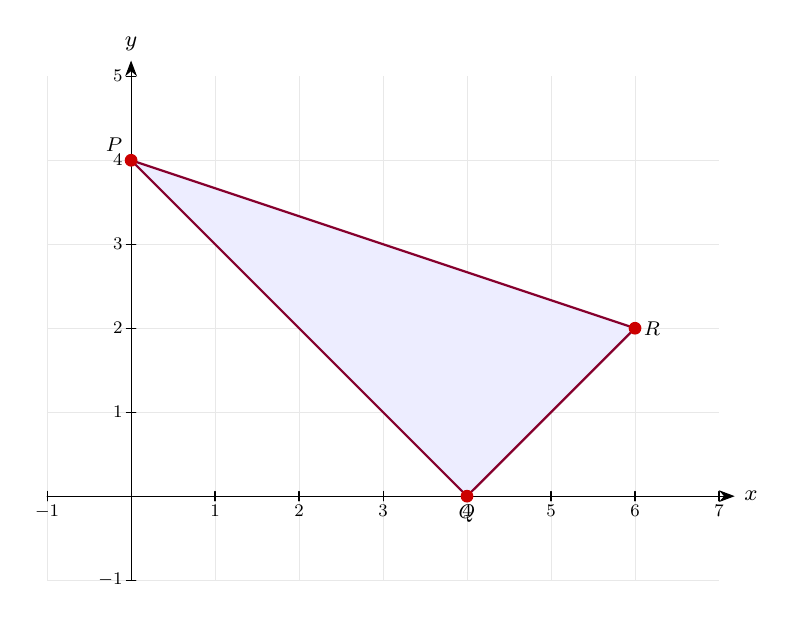
\begin{tikzpicture}[>={Stealth[length=2mm]},font=\footnotesize,line cap=round]
\begin{scope}
\clip (0,0) rectangle (8.533,6.4);
\draw[gray!18] (0,0) grid[xstep=1.067,ystep=1.067] (8.533,6.4);
\fill[blue!7] (1.067,5.333) -- (5.333,1.067) -- (7.467,3.2) -- cycle;
\draw[purple!70!black,thick] (1.067,5.333) -- (5.333,1.067) -- (7.467,3.2) -- cycle;
\end{scope}
\draw[->] (0,1.067) -- (8.733,1.067) node[right]{$x$};
\draw[->] (1.067,0) -- (1.067,6.6) node[above]{$y$};
\draw (0,1.007) -- (0,1.127) node[below=2pt,scale=0.8]{$-1$};
\draw (2.133,1.007) -- (2.133,1.127) node[below=2pt,scale=0.8]{$1$};
\draw (3.2,1.007) -- (3.2,1.127) node[below=2pt,scale=0.8]{$2$};
\draw (4.267,1.007) -- (4.267,1.127) node[below=2pt,scale=0.8]{$3$};
\draw (5.333,1.007) -- (5.333,1.127) node[below=2pt,scale=0.8]{$4$};
\draw (6.4,1.007) -- (6.4,1.127) node[below=2pt,scale=0.8]{$5$};
\draw (7.467,1.007) -- (7.467,1.127) node[below=2pt,scale=0.8]{$6$};
\draw (8.533,1.007) -- (8.533,1.127) node[below=2pt,scale=0.8]{$7$};
\draw (1.007,0) -- (1.127,0) node[left=2pt,scale=0.8]{$-1$};
\draw (1.007,2.133) -- (1.127,2.133) node[left=2pt,scale=0.8]{$1$};
\draw (1.007,3.2) -- (1.127,3.2) node[left=2pt,scale=0.8]{$2$};
\draw (1.007,4.267) -- (1.127,4.267) node[left=2pt,scale=0.8]{$3$};
\draw (1.007,5.333) -- (1.127,5.333) node[left=2pt,scale=0.8]{$4$};
\draw (1.007,6.4) -- (1.127,6.4) node[left=2pt,scale=0.8]{$5$};
\fill[red!80!black] (1.067,5.333) circle (2.3pt);
\node[above left,scale=0.9] at (1.067,5.333) {$P$};
\fill[red!80!black] (5.333,1.067) circle (2.3pt);
\node[below,scale=0.9] at (5.333,1.067) {$Q$};
\fill[red!80!black] (7.467,3.2) circle (2.3pt);
\node[right,scale=0.9] at (7.467,3.2) {$R$};
\end{tikzpicture}
}
\end{center}
\small The line(s) and key points shown on the coordinate plane.\normalsize

\medskip\hrule

\section*{Parallel and Perpendicular Lines 28\quad\small\texttt{(cg3-028)}}
\addcontentsline{toc}{section}{Parallel and Perpendicular Lines 28 (cg3-028)}
\textit{Difficulty: Foundation \quad\textbar\quad Marks: 8}

\question{Triangle \( ABC \) has vertices \( A(0, 0) \), \( B(4, 2) \) and \( C(2, 6) \). \\[3pt] (a) Find the equations of \( AB \), \( BC \) and \( AC \) in the form \( y = mx + c \). \\[3pt] (b) What type of triangle is \( ABC \)? Justify your answer.}

\textbf{Worked solution.}

\textit{Step 1: (a) Gradient of \( AB \):}
\[\begin{gathered}
m_{AB} = \dfrac{2-0}{4-0} = \dfrac{1}{2}; \quad y = \dfrac{1}{2}x
\end{gathered}\]
Since \( A \) is the origin, the line through \( A \) with gradient \( \tfrac{1}{2} \) has zero \( y \)-intercept.

\textit{Step 2: Gradient of \( BC \):}
\[\begin{gathered}
m_{BC} = \dfrac{6-2}{2-4} = \dfrac{4}{-2} = -2; \quad y = -2x + 10
\end{gathered}\]
Use point-slope through \( B(4, 2) \): \( y - 2 = -2(x - 4) \). Check: at \( x=4 \), \( y=-8+10=2 \checkmark \).

\textit{Step 3: Gradient of \( AC \):}
\[\begin{gathered}
m_{AC} = \dfrac{6-0}{2-0} = 3; \quad y = 3x
\end{gathered}\]
\( A \) is the origin, so again the line through \( A \) is \( y = 3x \).

\textit{Step 4: (b) Check perpendicularity: \( m_{AB} \times m_{BC} = \frac{1}{2} \times (-2) = -1 \).}
\[\begin{gathered}
m_{AB} \times m_{BC} = -1 \implies AB \perp BC
\end{gathered}\]
Triangle \( ABC \) is right-angled at \( B \).

\begin{answerbox}
\textbf{Final answer:}\quad (a) \(\displaystyle AB: y=\frac{1}{2}x\); \(\displaystyle BC: y=-2x+10\); \(\displaystyle AC: y=3x\); (b) Right-angled at \(\displaystyle B\) (since \(\displaystyle AB \perp BC\)).
\end{answerbox}
\textbf{Diagram.}

\begin{center}
\resizebox{\ifdim\width>\linewidth \linewidth\else \width\fi}{!}{%
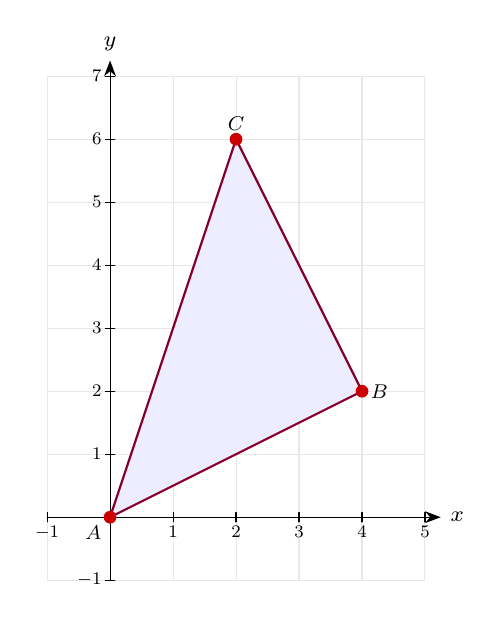
\begin{tikzpicture}[>={Stealth[length=2mm]},font=\footnotesize,line cap=round]
\begin{scope}
\clip (0,0) rectangle (4.8,6.4);
\draw[gray!18] (0,0) grid[xstep=0.8,ystep=0.8] (4.8,6.4);
\fill[blue!7] (0.8,0.8) -- (4,2.4) -- (2.4,5.6) -- cycle;
\draw[purple!70!black,thick] (0.8,0.8) -- (4,2.4) -- (2.4,5.6) -- cycle;
\end{scope}
\draw[->] (0,0.8) -- (5,0.8) node[right]{$x$};
\draw[->] (0.8,0) -- (0.8,6.6) node[above]{$y$};
\draw (0,0.74) -- (0,0.86) node[below=2pt,scale=0.8]{$-1$};
\draw (1.6,0.74) -- (1.6,0.86) node[below=2pt,scale=0.8]{$1$};
\draw (2.4,0.74) -- (2.4,0.86) node[below=2pt,scale=0.8]{$2$};
\draw (3.2,0.74) -- (3.2,0.86) node[below=2pt,scale=0.8]{$3$};
\draw (4,0.74) -- (4,0.86) node[below=2pt,scale=0.8]{$4$};
\draw (4.8,0.74) -- (4.8,0.86) node[below=2pt,scale=0.8]{$5$};
\draw (0.74,0) -- (0.86,0) node[left=2pt,scale=0.8]{$-1$};
\draw (0.74,1.6) -- (0.86,1.6) node[left=2pt,scale=0.8]{$1$};
\draw (0.74,2.4) -- (0.86,2.4) node[left=2pt,scale=0.8]{$2$};
\draw (0.74,3.2) -- (0.86,3.2) node[left=2pt,scale=0.8]{$3$};
\draw (0.74,4) -- (0.86,4) node[left=2pt,scale=0.8]{$4$};
\draw (0.74,4.8) -- (0.86,4.8) node[left=2pt,scale=0.8]{$5$};
\draw (0.74,5.6) -- (0.86,5.6) node[left=2pt,scale=0.8]{$6$};
\draw (0.74,6.4) -- (0.86,6.4) node[left=2pt,scale=0.8]{$7$};
\fill[red!80!black] (0.8,0.8) circle (2.3pt);
\node[below left,scale=0.9] at (0.8,0.8) {$A$};
\fill[red!80!black] (4,2.4) circle (2.3pt);
\node[right,scale=0.9] at (4,2.4) {$B$};
\fill[red!80!black] (2.4,5.6) circle (2.3pt);
\node[above,scale=0.9] at (2.4,5.6) {$C$};
\end{tikzpicture}
}
\end{center}
\small The line(s) and key points shown on the coordinate plane.\normalsize

\medskip\hrule

\section*{Parallel and Perpendicular Lines 29\quad\small\texttt{(cg3-029)}}
\addcontentsline{toc}{section}{Parallel and Perpendicular Lines 29 (cg3-029)}
\textit{Difficulty: Foundation \quad\textbar\quad Marks: 6}

\question{Point \( A = (2, 5) \). The line \( L \) has equation \( y = 3x - 4 \). Find the equation of the line through \( A \) perpendicular to \( L \), and find where it meets \( L \).}

\textbf{Worked solution.}

\textit{Step 1: Perpendicular gradient: \( m_\perp = -\frac{1}{3} \).}
\[\begin{gathered}
y - 5 = -\dfrac{1}{3}(x - 2) \implies y = -\dfrac{1}{3}x + \dfrac{17}{3}
\end{gathered}\]
Negative reciprocal of \( 3 \). Apply point-slope form through \( A(2, 5) \); expanding gives \( y = -\tfrac{1}{3}x + \tfrac{2}{3} + 5 = -\tfrac{1}{3}x + \tfrac{17}{3} \).

\textit{Step 2: Find intersection with \( y = 3x - 4 \):}
\[\begin{gathered}
3x - 4 = -\dfrac{1}{3}x + \dfrac{17}{3}
\end{gathered}\]
Set the two \( y \)-expressions equal --- at the intersection point both lines share the same \( (x, y) \).

\textit{Step 3: Multiply through by 3:}
\[\begin{gathered}
9x - 12 = -x + 17 \implies 10x = 29 \implies x = 2.9,\ y = 3(2.9) - 4 = 4.7
\end{gathered}\]
Multiplying by \( 3 \) clears the fractions. Then collect \( x \)-terms and substitute back into either line to find \( y \).

\begin{answerbox}
\textbf{Final answer:}\quad Perpendicular: \(\displaystyle y = -\dfrac{1}{3}x + \dfrac{17}{3}\); meets \(\displaystyle L\) at \(\displaystyle (2.9, 4.7)\)
\end{answerbox}
\textbf{Diagram.}

\begin{center}
\resizebox{\ifdim\width>\linewidth \linewidth\else \width\fi}{!}{%
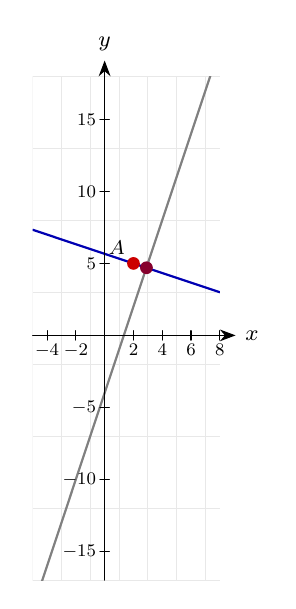
\begin{tikzpicture}[>={Stealth[length=2mm]},font=\footnotesize,line cap=round]
\begin{scope}
\clip (0,0) rectangle (2.377,6.4);
\draw[gray!18] (-0.183,-0.549) grid[xstep=0.366,ystep=0.914] (2.377,6.4);
\draw[gray,thick] (0,-0.366) -- (2.377,6.766);
\draw[blue!70!black,thick] (0,4.45) -- (2.377,3.657);
\end{scope}
\draw[->] (0,3.109) -- (2.577,3.109) node[right]{$x$};
\draw[->] (0.914,0) -- (0.914,6.6) node[above]{$y$};
\draw (0.183,3.049) -- (0.183,3.169) node[below=2pt,scale=0.8]{$-4$};
\draw (0.549,3.049) -- (0.549,3.169) node[below=2pt,scale=0.8]{$-2$};
\draw (1.28,3.049) -- (1.28,3.169) node[below=2pt,scale=0.8]{$2$};
\draw (1.646,3.049) -- (1.646,3.169) node[below=2pt,scale=0.8]{$4$};
\draw (2.011,3.049) -- (2.011,3.169) node[below=2pt,scale=0.8]{$6$};
\draw (2.377,3.049) -- (2.377,3.169) node[below=2pt,scale=0.8]{$8$};
\draw (0.854,0.366) -- (0.974,0.366) node[left=2pt,scale=0.8]{$-15$};
\draw (0.854,1.28) -- (0.974,1.28) node[left=2pt,scale=0.8]{$-10$};
\draw (0.854,2.194) -- (0.974,2.194) node[left=2pt,scale=0.8]{$-5$};
\draw (0.854,4.023) -- (0.974,4.023) node[left=2pt,scale=0.8]{$5$};
\draw (0.854,4.937) -- (0.974,4.937) node[left=2pt,scale=0.8]{$10$};
\draw (0.854,5.851) -- (0.974,5.851) node[left=2pt,scale=0.8]{$15$};
\fill[red!80!black] (1.28,4.023) circle (2.3pt);
\node[above left,scale=0.9] at (1.28,4.023) {$A$};
\fill[purple!70!black] (1.445,3.968) circle (2.3pt);
\end{tikzpicture}
}
\end{center}
\small The line(s) and key points shown on the coordinate plane.\normalsize

\medskip\hrule

\section*{Parallel and Perpendicular Lines 30\quad\small\texttt{(cg3-030)}}
\addcontentsline{toc}{section}{Parallel and Perpendicular Lines 30 (cg3-030)}
\textit{Difficulty: Foundation \quad\textbar\quad Marks: 6}

\question{Two lines are given: \( L_1: 2x - y + 4 = 0 \) and \( L_2: x + 2y - 3 = 0 \). \\[3pt] (a) Show that \( L_1 \) and \( L_2 \) are perpendicular. \\[3pt] (b) Find their point of intersection.}

\textbf{Worked solution.}

\textit{Step 1: (a) Rearrange each line.}
\[\begin{gathered}
L_1:\ y = 2x + 4 \implies m_1 = 2; \quad L_2:\ y = -\dfrac{1}{2}x + \dfrac{3}{2} \implies m_2 = -\dfrac{1}{2}
\end{gathered}\]
Isolate \( y \) in each equation to read off gradients.

\textit{Step 2: Product of gradients:}
\[\begin{gathered}
2 \times \left(-\dfrac{1}{2}\right) = -1 \implies L_1 \perp L_2 \checkmark
\end{gathered}\]
Two non-vertical lines are perpendicular if and only if the product of gradients is \( -1 \).

\textit{Step 3: (b) Solve simultaneously. From \( L_2 \): \( x = 3 - 2y \). Substitute into \( L_1 \):}
\[\begin{gathered}
2(3 - 2y) - y + 4 = 0 \implies 6 - 4y - y + 4 = 0 \implies 5y = 10 \implies y = 2,\ x = -1
\end{gathered}\]
Substitution eliminates \( x \). Expanding gives \( 10 - 5y = 0 \), so \( y = 2 \). Then \( x = 3 - 4 = -1 \).

\begin{answerbox}
\textbf{Final answer:}\quad (a) Shown --- gradients multiply to \(\displaystyle -1\); (b) Intersection at \(\displaystyle (-1, 2)\)
\end{answerbox}
\textbf{Diagram.}

\begin{center}
\resizebox{\ifdim\width>\linewidth \linewidth\else \width\fi}{!}{%
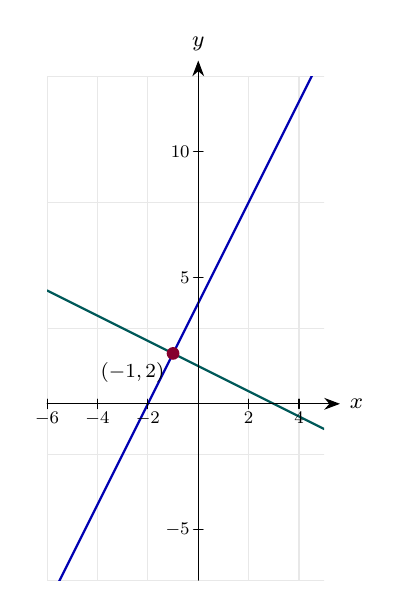
\begin{tikzpicture}[>={Stealth[length=2mm]},font=\footnotesize,line cap=round]
\begin{scope}
\clip (0,0) rectangle (3.52,6.4);
\draw[gray!18] (0,-0.96) grid[xstep=0.64,ystep=1.6] (3.52,6.4);
\draw[blue!70!black,thick] (0,-0.32) -- (3.52,6.72);
\draw[teal!70!black,thick] (0,3.68) -- (3.52,1.92);
\end{scope}
\draw[->] (0,2.24) -- (3.72,2.24) node[right]{$x$};
\draw[->] (1.92,0) -- (1.92,6.6) node[above]{$y$};
\draw (0,2.18) -- (0,2.3) node[below=2pt,scale=0.8]{$-6$};
\draw (0.64,2.18) -- (0.64,2.3) node[below=2pt,scale=0.8]{$-4$};
\draw (1.28,2.18) -- (1.28,2.3) node[below=2pt,scale=0.8]{$-2$};
\draw (2.56,2.18) -- (2.56,2.3) node[below=2pt,scale=0.8]{$2$};
\draw (3.2,2.18) -- (3.2,2.3) node[below=2pt,scale=0.8]{$4$};
\draw (1.86,0.64) -- (1.98,0.64) node[left=2pt,scale=0.8]{$-5$};
\draw (1.86,3.84) -- (1.98,3.84) node[left=2pt,scale=0.8]{$5$};
\draw (1.86,5.44) -- (1.98,5.44) node[left=2pt,scale=0.8]{$10$};
\fill[purple!70!black] (1.6,2.88) circle (2.3pt);
\node[below left,scale=0.9] at (1.6,2.88) {$(-1,2)$};
\end{tikzpicture}
}
\end{center}
\small The line(s) and key points shown on the coordinate plane.\normalsize

\medskip\hrule

\section*{Parallel and Perpendicular Lines 31\quad\small\texttt{(cg3-031)}}
\addcontentsline{toc}{section}{Parallel and Perpendicular Lines 31 (cg3-031)}
\textit{Difficulty: Foundation \quad\textbar\quad Marks: 8}

\question{Line \( L_1 \) passes through \( A(1, 3) \) and \( B(5, 11) \). \\[3pt] (a) Find the equation of \( L_1 \) in the form \( y = mx + c \). \\[3pt] (b) Line \( L_2 \) is parallel to \( L_1 \) and passes through \( C(3, -2) \). Find the equation of \( L_2 \). \\[3pt] (c) Line \( L_3 \) is perpendicular to \( L_1 \) and passes through \( B \). Find the equation of \( L_3 \).}

\textbf{Worked solution.}

\textit{Step 1: (a) Gradient of \( L_1 \):}
\[\begin{gathered}
m = \dfrac{11-3}{5-1} = 2; \quad 3 = 2(1) + c \implies c = 1 \implies y = 2x + 1
\end{gathered}\]
Apply the gradient formula to \( A \) and \( B \). Then substitute \( A(1, 3) \) into \( y = 2x + c \) to find the intercept.

\textit{Step 2: (b) \( L_2 \) has gradient 2, passes through \( C(3, -2) \):}
\[\begin{gathered}
-2 = 2(3) + c \implies c = -8 \implies y = 2x - 8
\end{gathered}\]
Parallel lines share gradients. Substitute \( C \): \( c = -2 - 6 = -8 \).

\textit{Step 3: (c) \( L_3 \) has gradient \( -\frac{1}{2} \), passes through \( B(5, 11) \):}
\[\begin{gathered}
11 = -\dfrac{1}{2}(5) + c \implies c = \dfrac{27}{2} \implies y = -\dfrac{1}{2}x + \dfrac{27}{2}
\end{gathered}\]
Perpendicular gradient is the negative reciprocal of \( 2 \). Then \( c = 11 + \tfrac{5}{2} = \tfrac{22}{2} + \tfrac{5}{2} = \tfrac{27}{2} \).

\begin{answerbox}
\textbf{Final answer:}\quad (a) \(\displaystyle y = 2x + 1\); (b) \(\displaystyle y = 2x - 8\); (c) \(\displaystyle y = -\dfrac{1}{2}x + \dfrac{27}{2}\)
\end{answerbox}
\textbf{Diagram.}

\begin{center}
\resizebox{\ifdim\width>\linewidth \linewidth\else \width\fi}{!}{%
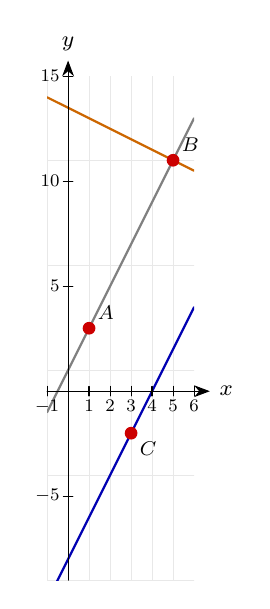
\begin{tikzpicture}[>={Stealth[length=2mm]},font=\footnotesize,line cap=round]
\begin{scope}
\clip (0,0) rectangle (1.867,6.4);
\draw[gray!18] (0,-0.267) grid[xstep=0.267,ystep=1.333] (1.867,6.4);
\draw[gray,thick] (0,2.133) -- (1.867,5.867);
\draw[blue!70!black,thick] (0,-0.267) -- (1.867,3.467);
\draw[orange!80!black,thick] (0,6.133) -- (1.867,5.2);
\end{scope}
\draw[->] (0,2.4) -- (2.067,2.4) node[right]{$x$};
\draw[->] (0.267,0) -- (0.267,6.6) node[above]{$y$};
\draw (0,2.34) -- (0,2.46) node[below=2pt,scale=0.8]{$-1$};
\draw (0.533,2.34) -- (0.533,2.46) node[below=2pt,scale=0.8]{$1$};
\draw (0.8,2.34) -- (0.8,2.46) node[below=2pt,scale=0.8]{$2$};
\draw (1.067,2.34) -- (1.067,2.46) node[below=2pt,scale=0.8]{$3$};
\draw (1.333,2.34) -- (1.333,2.46) node[below=2pt,scale=0.8]{$4$};
\draw (1.6,2.34) -- (1.6,2.46) node[below=2pt,scale=0.8]{$5$};
\draw (1.867,2.34) -- (1.867,2.46) node[below=2pt,scale=0.8]{$6$};
\draw (0.207,1.067) -- (0.327,1.067) node[left=2pt,scale=0.8]{$-5$};
\draw (0.207,3.733) -- (0.327,3.733) node[left=2pt,scale=0.8]{$5$};
\draw (0.207,5.067) -- (0.327,5.067) node[left=2pt,scale=0.8]{$10$};
\draw (0.207,6.4) -- (0.327,6.4) node[left=2pt,scale=0.8]{$15$};
\fill[red!80!black] (0.533,3.2) circle (2.3pt);
\node[above right,scale=0.9] at (0.533,3.2) {$A$};
\fill[red!80!black] (1.6,5.333) circle (2.3pt);
\node[above right,scale=0.9] at (1.6,5.333) {$B$};
\fill[red!80!black] (1.067,1.867) circle (2.3pt);
\node[below right,scale=0.9] at (1.067,1.867) {$C$};
\end{tikzpicture}
}
\end{center}
\small The line(s) and key points shown on the coordinate plane.\normalsize

\medskip\hrule

\section*{Parallel and Perpendicular Lines 32\quad\small\texttt{(cg3-032)}}
\addcontentsline{toc}{section}{Parallel and Perpendicular Lines 32 (cg3-032)}
\textit{Difficulty: Foundation \quad\textbar\quad Marks: 8}

\question{The line \( L \) has equation \( 3x + 4y - 24 = 0 \). \\[3pt] (a) Find where \( L \) crosses the axes. \\[3pt] (b) Find the equation of the line parallel to \( L \) that passes through \( (4, -1) \). Give your answer in the form \( ax + by + c = 0 \). \\[3pt] (c) Find the equation of the line perpendicular to \( L \) that passes through \( (0, 0) \). Give your answer in the form \( y = mx \).}

\textbf{Worked solution.}

\textit{Step 1: (a) \( x \)-intercept (set \( y=0 \)): \( 3x = 24 \implies x = 8 \). \( y \)-intercept (set \( x=0 \)): \( 4y = 24 \implies y = 6 \).}
\[\begin{gathered}
x\text{-intercept}: (8, 0); \quad y\text{-intercept}: (0, 6)
\end{gathered}\]
Setting one variable to zero gives the intercept on the other axis directly.

\textit{Step 2: (b) Gradient of \( L \): \( m = -\frac{3}{4} \). Parallel line through \( (4, -1) \):}
\[\begin{gathered}
-1 = -\dfrac{3}{4}(4) + c \implies c = 2 \implies y = -\dfrac{3}{4}x + 2 \implies 3x + 4y - 8 = 0
\end{gathered}\]
From \( 4y = -3x + 24 \), the gradient is \( -\tfrac{3}{4} \). Substitute the point, then multiply by \( 4 \) and rearrange to integer form.

\textit{Step 3: (c) Perpendicular gradient: \( m_\perp = \frac{4}{3} \). Through \( (0, 0) \):}
\[\begin{gathered}
y = \dfrac{4}{3}x
\end{gathered}\]
Through the origin, \( c = 0 \), giving the required form \( y = mx \) directly.

\begin{answerbox}
\textbf{Final answer:}\quad (a) \(\displaystyle (8,0)\) and \(\displaystyle (0,6)\); (b) \(\displaystyle 3x+4y-8=0\); (c) \(\displaystyle y=\dfrac{4}{3}x\)
\end{answerbox}
\textbf{Diagram.}

\begin{center}
\resizebox{\ifdim\width>\linewidth \linewidth\else \width\fi}{!}{%
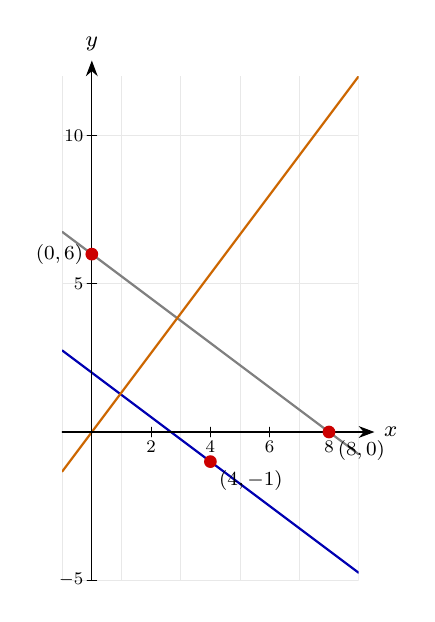
\begin{tikzpicture}[>={Stealth[length=2mm]},font=\footnotesize,line cap=round]
\begin{scope}
\clip (0,0) rectangle (3.765,6.4);
\draw[gray!18] (-0.376,0) grid[xstep=0.753,ystep=1.882] (3.765,6.4);
\draw[gray,thick] (0,4.424) -- (3.765,1.6);
\draw[blue!70!black,thick] (0,2.918) -- (3.765,0.094);
\draw[orange!80!black,thick] (0,1.38) -- (3.765,6.4);
\end{scope}
\draw[->] (0,1.882) -- (3.965,1.882) node[right]{$x$};
\draw[->] (0.376,0) -- (0.376,6.6) node[above]{$y$};
\draw (1.129,1.822) -- (1.129,1.942) node[below=2pt,scale=0.8]{$2$};
\draw (1.882,1.822) -- (1.882,1.942) node[below=2pt,scale=0.8]{$4$};
\draw (2.635,1.822) -- (2.635,1.942) node[below=2pt,scale=0.8]{$6$};
\draw (3.388,1.822) -- (3.388,1.942) node[below=2pt,scale=0.8]{$8$};
\draw (0.316,0) -- (0.436,0) node[left=2pt,scale=0.8]{$-5$};
\draw (0.316,3.765) -- (0.436,3.765) node[left=2pt,scale=0.8]{$5$};
\draw (0.316,5.647) -- (0.436,5.647) node[left=2pt,scale=0.8]{$10$};
\fill[red!80!black] (3.388,1.882) circle (2.3pt);
\node[below right,scale=0.9] at (3.388,1.882) {$(8,0)$};
\fill[red!80!black] (0.376,4.141) circle (2.3pt);
\node[left,scale=0.9] at (0.376,4.141) {$(0,6)$};
\fill[red!80!black] (1.882,1.506) circle (2.3pt);
\node[below right,scale=0.9] at (1.882,1.506) {$(4,-1)$};
\end{tikzpicture}
}
\end{center}
\small The line(s) and key points shown on the coordinate plane.\normalsize

\medskip\hrule

\section*{Parallel and Perpendicular Lines 33\quad\small\texttt{(cg3-033)}}
\addcontentsline{toc}{section}{Parallel and Perpendicular Lines 33 (cg3-033)}
\textit{Difficulty: Foundation \quad\textbar\quad Marks: 8}

\question{The vertices of a quadrilateral are \( A(0, 2) \), \( B(4, 4) \), \( C(6, 0) \) and \( D(2, -2) \). \\[3pt] (a) Find the gradients of all four sides. \\[3pt] (b) Show that \( ABCD \) is a rectangle.}

\textbf{Worked solution.}

\textit{Step 1: (a) Gradient of each side:}
\[\begin{gathered}
m_{AB} = \dfrac{4-2}{4-0} = \dfrac{1}{2}, \quad m_{BC} = \dfrac{0-4}{6-4} = -2
\end{gathered}\]
Apply the gradient formula \( m = \frac{y_2 - y_1}{x_2 - x_1} \) to each pair of vertices in turn.

\[\begin{gathered}
m_{CD} = \dfrac{-2-0}{2-6} = \dfrac{-2}{-4} = \dfrac{1}{2}, \quad m_{DA} = \dfrac{2-(-2)}{0-2} = -2
\end{gathered}\]
Watch the double negatives. For \( m_{CD} \) both numerator and denominator are negative, giving a positive result. For \( m_{DA} \), \( 2 - (-2) = 4 \).

\textit{Step 3: (b) \( AB \parallel CD \) (both gradient \( \frac{1}{2} \)) and \( BC \parallel DA \) (both gradient \( -2 \)), so \( ABCD \) is a parallelogram.}
\[\begin{gathered}
m_{AB} \times m_{BC} = \dfrac{1}{2} \times (-2) = -1
\end{gathered}\]
Adjacent sides are perpendicular, so the parallelogram is a rectangle. $\checkmark$

\begin{answerbox}
\textbf{Final answer:}\quad (a) \(\displaystyle m_{AB}=m_{CD}=\frac{1}{2}\), \(\displaystyle m_{BC}=m_{DA}=-2\); (b) Opposite sides parallel and adjacent sides perpendicular $\Rightarrow$ rectangle.
\end{answerbox}
\textbf{Diagram.}

\begin{center}
\resizebox{\ifdim\width>\linewidth \linewidth\else \width\fi}{!}{%
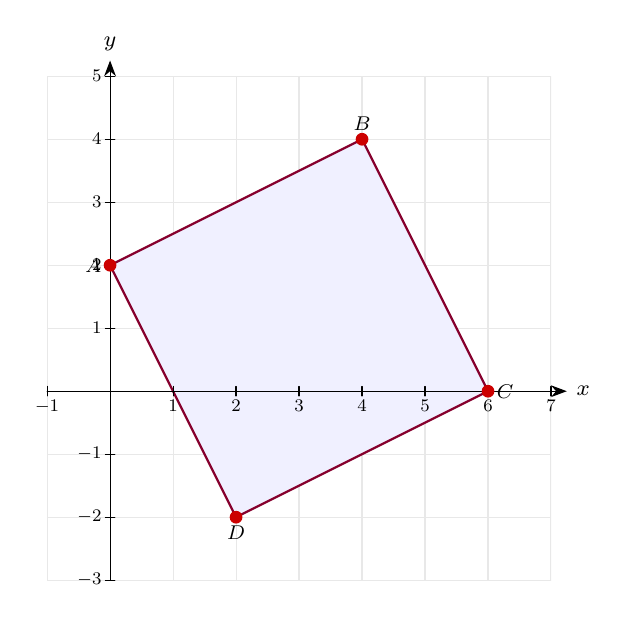
\begin{tikzpicture}[>={Stealth[length=2mm]},font=\footnotesize,line cap=round]
\begin{scope}
\clip (0,0) rectangle (6.4,6.4);
\draw[gray!18] (0,0) grid[xstep=0.8,ystep=0.8] (6.4,6.4);
\fill[blue!6] (0.8,4) -- (4,5.6) -- (5.6,2.4) -- (2.4,0.8) -- cycle;
\draw[purple!70!black,thick] (0.8,4) -- (4,5.6) -- (5.6,2.4) -- (2.4,0.8) -- cycle;
\end{scope}
\draw[->] (0,2.4) -- (6.6,2.4) node[right]{$x$};
\draw[->] (0.8,0) -- (0.8,6.6) node[above]{$y$};
\draw (0,2.34) -- (0,2.46) node[below=2pt,scale=0.8]{$-1$};
\draw (1.6,2.34) -- (1.6,2.46) node[below=2pt,scale=0.8]{$1$};
\draw (2.4,2.34) -- (2.4,2.46) node[below=2pt,scale=0.8]{$2$};
\draw (3.2,2.34) -- (3.2,2.46) node[below=2pt,scale=0.8]{$3$};
\draw (4,2.34) -- (4,2.46) node[below=2pt,scale=0.8]{$4$};
\draw (4.8,2.34) -- (4.8,2.46) node[below=2pt,scale=0.8]{$5$};
\draw (5.6,2.34) -- (5.6,2.46) node[below=2pt,scale=0.8]{$6$};
\draw (6.4,2.34) -- (6.4,2.46) node[below=2pt,scale=0.8]{$7$};
\draw (0.74,0) -- (0.86,0) node[left=2pt,scale=0.8]{$-3$};
\draw (0.74,0.8) -- (0.86,0.8) node[left=2pt,scale=0.8]{$-2$};
\draw (0.74,1.6) -- (0.86,1.6) node[left=2pt,scale=0.8]{$-1$};
\draw (0.74,3.2) -- (0.86,3.2) node[left=2pt,scale=0.8]{$1$};
\draw (0.74,4) -- (0.86,4) node[left=2pt,scale=0.8]{$2$};
\draw (0.74,4.8) -- (0.86,4.8) node[left=2pt,scale=0.8]{$3$};
\draw (0.74,5.6) -- (0.86,5.6) node[left=2pt,scale=0.8]{$4$};
\draw (0.74,6.4) -- (0.86,6.4) node[left=2pt,scale=0.8]{$5$};
\fill[red!80!black] (0.8,4) circle (2.3pt);
\node[left,scale=0.9] at (0.8,4) {$A$};
\fill[red!80!black] (4,5.6) circle (2.3pt);
\node[above,scale=0.9] at (4,5.6) {$B$};
\fill[red!80!black] (5.6,2.4) circle (2.3pt);
\node[right,scale=0.9] at (5.6,2.4) {$C$};
\fill[red!80!black] (2.4,0.8) circle (2.3pt);
\node[below,scale=0.9] at (2.4,0.8) {$D$};
\end{tikzpicture}
}
\end{center}
\small The line(s) and key points shown on the coordinate plane.\normalsize

\medskip\hrule

\section*{Parallel and Perpendicular Lines 34\quad\small\texttt{(cg3-034)}}
\addcontentsline{toc}{section}{Parallel and Perpendicular Lines 34 (cg3-034)}
\textit{Difficulty: Foundation \quad\textbar\quad Marks: 9}

\question{Line \( L_1 \) has equation \( y = \dfrac{1}{2}x + 3 \). Line \( L_2 \) is perpendicular to \( L_1 \) and passes through \( (4, 1) \). \\[3pt] (a) Find the equation of \( L_2 \) in the form \( ax + by + c = 0 \). \\[3pt] (b) Find the coordinates of the point where \( L_1 \) and \( L_2 \) intersect. \\[3pt] (c) Find the exact distance between the point \( (4, 1) \) and the intersection point.}

\textbf{Worked solution.}

\textit{Step 1: (a) Perpendicular gradient: \( m_\perp = -2 \). Through \( (4, 1) \):}
\[\begin{gathered}
1 = -2(4) + c \implies c = 9 \implies y = -2x + 9 \implies 2x + y - 9 = 0
\end{gathered}\]
Negative reciprocal of \( \tfrac{1}{2} \) is \( -2 \). Substitute the given point to find \( c \), then rearrange to the required form.

\textit{Step 2: (b) Solve \( y = \frac{1}{2}x + 3 \) and \( y = -2x + 9 \) simultaneously:}
\[\begin{gathered}
\dfrac{1}{2}x + 3 = -2x + 9 \implies \dfrac{5}{2}x = 6 \implies x = \dfrac{12}{5},\ y = -2\left(\dfrac{12}{5}\right)+9 = \dfrac{21}{5}
\end{gathered}\]
Set the \( y \)-expressions equal. Collecting \( x \)-terms: \( \tfrac{1}{2}x + 2x = \tfrac{5}{2}x \). Then divide by \( \tfrac{5}{2} \), i.e. multiply by \( \tfrac{2}{5} \).

\textit{Step 3: (c) Distance from \( (4, 1) \) to \( \left(\frac{12}{5}, \frac{21}{5}\right) \):}
\[\begin{gathered}
d = \sqrt{\left(4 - \dfrac{12}{5}\right)^2 + \left(1 - \dfrac{21}{5}\right)^2} = \sqrt{\left(\dfrac{8}{5}\right)^2 + \left(-\dfrac{16}{5}\right)^2} = \sqrt{\dfrac{64 + 256}{25}} = \sqrt{\dfrac{320}{25}} = \dfrac{8\sqrt{5}}{5}
\end{gathered}\]
Apply the distance formula (Pythagoras on the coordinate differences). Convert to common fifths: \( 4 = \tfrac{20}{5} \) and \( 1 = \tfrac{5}{5} \). \( \sqrt{320} = \sqrt{64 \times 5} = 8\sqrt{5} \).

\begin{answerbox}
\textbf{Final answer:}\quad (a) \(\displaystyle 2x+y-9=0\); (b) \(\displaystyle \left(\dfrac{12}{5}, \dfrac{21}{5}\right)\); (c) \(\displaystyle \dfrac{8\sqrt{5}}{5}\)
\end{answerbox}
\textbf{Diagram.}

\begin{center}
\resizebox{\ifdim\width>\linewidth \linewidth\else \width\fi}{!}{%
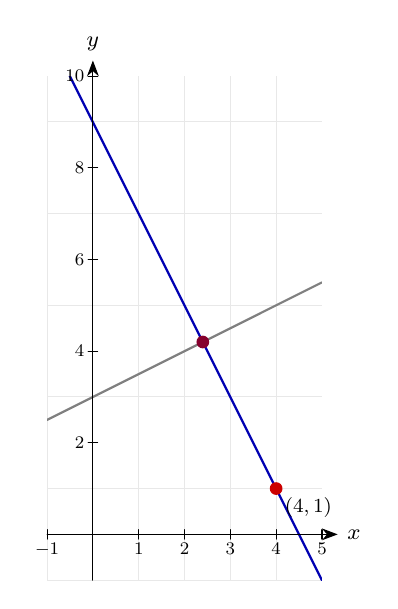
\begin{tikzpicture}[>={Stealth[length=2mm]},font=\footnotesize,line cap=round]
\begin{scope}
\clip (0,0) rectangle (3.491,6.4);
\draw[gray!18] (0,-0.582) grid[xstep=0.582,ystep=1.164] (3.491,6.4);
\draw[gray,thick] (0,2.036) -- (3.491,3.782);
\draw[blue!70!black,thick] (0,6.982) -- (3.491,0);
\end{scope}
\draw[->] (0,0.582) -- (3.691,0.582) node[right]{$x$};
\draw[->] (0.582,0) -- (0.582,6.6) node[above]{$y$};
\draw (0,0.522) -- (0,0.642) node[below=2pt,scale=0.8]{$-1$};
\draw (1.164,0.522) -- (1.164,0.642) node[below=2pt,scale=0.8]{$1$};
\draw (1.745,0.522) -- (1.745,0.642) node[below=2pt,scale=0.8]{$2$};
\draw (2.327,0.522) -- (2.327,0.642) node[below=2pt,scale=0.8]{$3$};
\draw (2.909,0.522) -- (2.909,0.642) node[below=2pt,scale=0.8]{$4$};
\draw (3.491,0.522) -- (3.491,0.642) node[below=2pt,scale=0.8]{$5$};
\draw (0.522,1.745) -- (0.642,1.745) node[left=2pt,scale=0.8]{$2$};
\draw (0.522,2.909) -- (0.642,2.909) node[left=2pt,scale=0.8]{$4$};
\draw (0.522,4.073) -- (0.642,4.073) node[left=2pt,scale=0.8]{$6$};
\draw (0.522,5.236) -- (0.642,5.236) node[left=2pt,scale=0.8]{$8$};
\draw (0.522,6.4) -- (0.642,6.4) node[left=2pt,scale=0.8]{$10$};
\fill[red!80!black] (2.909,1.164) circle (2.3pt);
\node[below right,scale=0.9] at (2.909,1.164) {$(4,1)$};
\fill[purple!70!black] (1.978,3.025) circle (2.3pt);
\end{tikzpicture}
}
\end{center}
\small The line(s) and key points shown on the coordinate plane.\normalsize

\medskip\hrule

\section*{Parallel and Perpendicular Lines 35\quad\small\texttt{(cg3-035)}}
\addcontentsline{toc}{section}{Parallel and Perpendicular Lines 35 (cg3-035)}
\textit{Difficulty: Foundation \quad\textbar\quad Marks: 9}

\question{Points \( A(2, 7) \), \( B(8, 5) \) and \( C(k, 1) \) are given. \\[3pt] (a) Find the equation of the perpendicular bisector of \( AB \). \\[3pt] (b) Given that \( C \) lies on the perpendicular bisector of \( AB \), find the value of \( k \). \\[3pt] (c) Find the exact distance \( AC \).}

\textbf{Worked solution.}

\textit{Step 1: (a) Midpoint of \( AB \):}
\[\begin{gathered}
M = \left(\dfrac{2+8}{2},\ \dfrac{7+5}{2}\right) = (5,\ 6)
\end{gathered}\]
Average the endpoint coordinates. The perpendicular bisector must pass through this midpoint.

\textit{Step 2: Gradient of \( AB \):}
\[\begin{gathered}
m_{AB} = \dfrac{5-7}{8-2} = -\dfrac{1}{3} \implies m_\perp = 3
\end{gathered}\]
Use the gradient formula, then take the negative reciprocal: flip \( -\tfrac{1}{3} \) and change sign to get \( 3 \).

\textit{Step 3: Perpendicular bisector through \( M(5,6) \) with gradient 3:}
\[\begin{gathered}
6 = 3(5) + c \implies c = -9 \implies y = 3x - 9
\end{gathered}\]
Substitute the midpoint to find \( c \): \( c = 6 - 15 = -9 \).

\textit{Step 4: (b) Substitute \( C(k, 1) \) into \( y = 3x - 9 \):}
\[\begin{gathered}
1 = 3k - 9 \implies 3k = 10 \implies k = \dfrac{10}{3}
\end{gathered}\]
Since \( C \) lies on the bisector its coordinates satisfy the equation. Solve the resulting linear equation in \( k \).

\textit{Step 5: (c) \( A = (2, 7) \), \( C = \left(\frac{10}{3}, 1\right) \):}
\[\begin{gathered}
AC = \sqrt{\left(\dfrac{10}{3}-2\right)^2 + (1-7)^2} = \sqrt{\left(\dfrac{4}{3}\right)^2 + 36} = \sqrt{\dfrac{16}{9} + \dfrac{324}{9}} = \sqrt{\dfrac{340}{9}} = \dfrac{2\sqrt{85}}{3}
\end{gathered}\]
Distance formula. Convert \( 36 \) to ninths so the surds combine: \( 36 = \tfrac{324}{9} \). Finally \( \sqrt{340} = \sqrt{4 \times 85} = 2\sqrt{85} \), and \( \sqrt{9} = 3 \).

\begin{answerbox}
\textbf{Final answer:}\quad (a) \(\displaystyle y = 3x - 9\); (b) \(\displaystyle k = \dfrac{10}{3}\); (c) \(\displaystyle AC = \dfrac{2\sqrt{85}}{3}\)
\end{answerbox}
\textbf{Diagram.}

\begin{center}
\resizebox{\ifdim\width>\linewidth \linewidth\else \width\fi}{!}{%
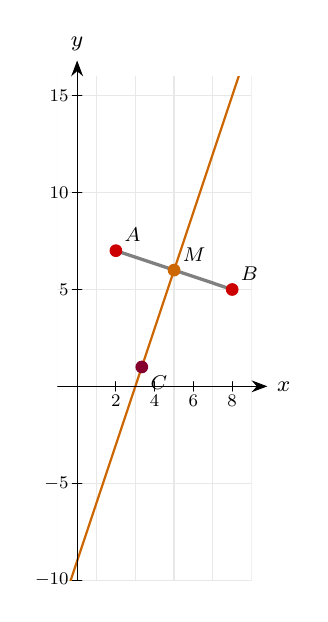
\begin{tikzpicture}[>={Stealth[length=2mm]},font=\footnotesize,line cap=round]
\begin{scope}
\clip (0,0) rectangle (2.462,6.4);
\draw[gray!18] (-0.246,0) grid[xstep=0.492,ystep=1.231] (2.462,6.4);
\draw[orange!80!black,thick] (0,-0.492) -- (2.462,6.892);
\draw[gray,very thick] (0.738,4.185) -- (2.215,3.692);
\end{scope}
\draw[->] (0,2.462) -- (2.662,2.462) node[right]{$x$};
\draw[->] (0.246,0) -- (0.246,6.6) node[above]{$y$};
\draw (0.738,2.402) -- (0.738,2.522) node[below=2pt,scale=0.8]{$2$};
\draw (1.231,2.402) -- (1.231,2.522) node[below=2pt,scale=0.8]{$4$};
\draw (1.723,2.402) -- (1.723,2.522) node[below=2pt,scale=0.8]{$6$};
\draw (2.215,2.402) -- (2.215,2.522) node[below=2pt,scale=0.8]{$8$};
\draw (0.186,0) -- (0.306,0) node[left=2pt,scale=0.8]{$-10$};
\draw (0.186,1.231) -- (0.306,1.231) node[left=2pt,scale=0.8]{$-5$};
\draw (0.186,3.692) -- (0.306,3.692) node[left=2pt,scale=0.8]{$5$};
\draw (0.186,4.923) -- (0.306,4.923) node[left=2pt,scale=0.8]{$10$};
\draw (0.186,6.154) -- (0.306,6.154) node[left=2pt,scale=0.8]{$15$};
\fill[red!80!black] (0.738,4.185) circle (2.3pt);
\node[above right,scale=0.9] at (0.738,4.185) {$A$};
\fill[red!80!black] (2.215,3.692) circle (2.3pt);
\node[above right,scale=0.9] at (2.215,3.692) {$B$};
\fill[orange!80!black] (1.477,3.938) circle (2.3pt);
\node[above right,scale=0.9] at (1.477,3.938) {$M$};
\fill[purple!70!black] (1.067,2.708) circle (2.3pt);
\node[below right,scale=0.9] at (1.067,2.708) {$C$};
\end{tikzpicture}
}
\end{center}
\small The line(s) and key points shown on the coordinate plane.\normalsize

\medskip\hrule

\section*{Parallel and Perpendicular Lines 36\quad\small\texttt{(cg3-036)}}
\addcontentsline{toc}{section}{Parallel and Perpendicular Lines 36 (cg3-036)}
\textit{Difficulty: Foundation \quad\textbar\quad Marks: 2}

\question{Find the equation of the line parallel to \( y = 4x - 1 \) that passes through \( (2, 3) \).}

\textbf{Worked solution.}

\textit{Step 1: Same gradient}
\[\begin{gathered}
m = 4
\end{gathered}\]
Parallel lines share gradients, so the new line also has gradient \( 4 \).

\textit{Step 2: Point-slope}
\[\begin{gathered}
y - 3 = 4(x - 2) \implies y = 4x - 5
\end{gathered}\]
Apply \( y - y_1 = m(x - x_1) \) through \( (2, 3) \), then expand and simplify.

\begin{answerbox}
\textbf{Final answer:}\quad \(\displaystyle y = 4x - 5\)
\end{answerbox}
\textbf{Diagram.}

\begin{center}
\resizebox{\ifdim\width>\linewidth \linewidth\else \width\fi}{!}{%
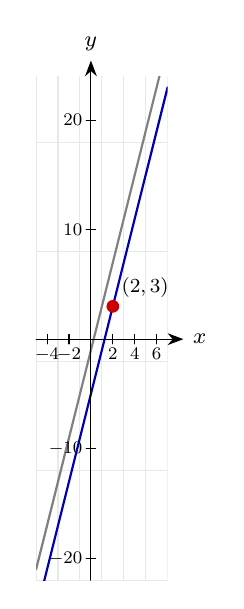
\begin{tikzpicture}[>={Stealth[length=2mm]},font=\footnotesize,line cap=round]
\begin{scope}
\clip (0,0) rectangle (1.67,6.4);
\draw[gray!18] (-0.139,-1.113) grid[xstep=0.278,ystep=1.391] (1.67,6.4);
\draw[gray,thick] (0,0.139) -- (1.67,6.817);
\draw[blue!70!black,thick] (0,-0.417) -- (1.67,6.261);
\end{scope}
\draw[->] (0,3.061) -- (1.87,3.061) node[right]{$x$};
\draw[->] (0.696,0) -- (0.696,6.6) node[above]{$y$};
\draw (0.139,3.001) -- (0.139,3.121) node[below=2pt,scale=0.8]{$-4$};
\draw (0.417,3.001) -- (0.417,3.121) node[below=2pt,scale=0.8]{$-2$};
\draw (0.974,3.001) -- (0.974,3.121) node[below=2pt,scale=0.8]{$2$};
\draw (1.252,3.001) -- (1.252,3.121) node[below=2pt,scale=0.8]{$4$};
\draw (1.53,3.001) -- (1.53,3.121) node[below=2pt,scale=0.8]{$6$};
\draw (0.636,0.278) -- (0.756,0.278) node[left=2pt,scale=0.8]{$-20$};
\draw (0.636,1.67) -- (0.756,1.67) node[left=2pt,scale=0.8]{$-10$};
\draw (0.636,4.452) -- (0.756,4.452) node[left=2pt,scale=0.8]{$10$};
\draw (0.636,5.843) -- (0.756,5.843) node[left=2pt,scale=0.8]{$20$};
\fill[red!80!black] (0.974,3.478) circle (2.3pt);
\node[above right,scale=0.9] at (0.974,3.478) {$(2,3)$};
\end{tikzpicture}
}
\end{center}
\small The line(s) and key points shown on the coordinate plane.\normalsize

\medskip\hrule

\section*{Parallel and Perpendicular Lines 37\quad\small\texttt{(cg3-037)}}
\addcontentsline{toc}{section}{Parallel and Perpendicular Lines 37 (cg3-037)}
\textit{Difficulty: Foundation \quad\textbar\quad Marks: 3}

\question{Find the equation of the line perpendicular to \( y = 3x + 2 \) passing through \( (6, 1) \).}

\textbf{Worked solution.}

\textit{Step 1: Perpendicular gradient}
\[\begin{gathered}
m = -\frac{1}{3}
\end{gathered}\]
Negative reciprocal of 3.

\textit{Step 2: Equation}
\[\begin{gathered}
y - 1 = -\frac{1}{3}(x - 6) \implies y = -\frac{1}{3}x + 3
\end{gathered}\]
Expand: \( -\tfrac{1}{3}(x - 6) = -\tfrac{1}{3}x + 2 \), then add \( 1 \) to both sides.

\begin{answerbox}
\textbf{Final answer:}\quad \(\displaystyle y = -\frac{1}{3}x + 3\)
\end{answerbox}
\textbf{Diagram.}

\begin{center}
\resizebox{\ifdim\width>\linewidth \linewidth\else \width\fi}{!}{%
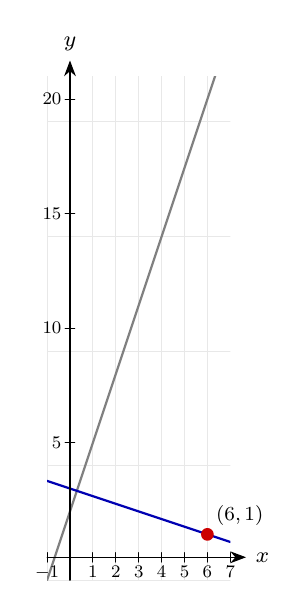
\begin{tikzpicture}[>={Stealth[length=2mm]},font=\footnotesize,line cap=round]
\begin{scope}
\clip (0,0) rectangle (2.327,6.4);
\draw[gray!18] (0,-1.164) grid[xstep=0.291,ystep=1.455] (2.327,6.4);
\draw[gray,thick] (0,0) -- (2.327,6.982);
\draw[blue!70!black,thick] (0,1.261) -- (2.327,0.485);
\end{scope}
\draw[->] (0,0.291) -- (2.527,0.291) node[right]{$x$};
\draw[->] (0.291,0) -- (0.291,6.6) node[above]{$y$};
\draw (0,0.231) -- (0,0.351) node[below=2pt,scale=0.8]{$-1$};
\draw (0.582,0.231) -- (0.582,0.351) node[below=2pt,scale=0.8]{$1$};
\draw (0.873,0.231) -- (0.873,0.351) node[below=2pt,scale=0.8]{$2$};
\draw (1.164,0.231) -- (1.164,0.351) node[below=2pt,scale=0.8]{$3$};
\draw (1.455,0.231) -- (1.455,0.351) node[below=2pt,scale=0.8]{$4$};
\draw (1.745,0.231) -- (1.745,0.351) node[below=2pt,scale=0.8]{$5$};
\draw (2.036,0.231) -- (2.036,0.351) node[below=2pt,scale=0.8]{$6$};
\draw (2.327,0.231) -- (2.327,0.351) node[below=2pt,scale=0.8]{$7$};
\draw (0.231,1.745) -- (0.351,1.745) node[left=2pt,scale=0.8]{$5$};
\draw (0.231,3.2) -- (0.351,3.2) node[left=2pt,scale=0.8]{$10$};
\draw (0.231,4.655) -- (0.351,4.655) node[left=2pt,scale=0.8]{$15$};
\draw (0.231,6.109) -- (0.351,6.109) node[left=2pt,scale=0.8]{$20$};
\fill[red!80!black] (2.036,0.582) circle (2.3pt);
\node[above right,scale=0.9] at (2.036,0.582) {$(6,1)$};
\end{tikzpicture}
}
\end{center}
\small The line(s) and key points shown on the coordinate plane.\normalsize

\medskip\hrule

\section*{Parallel and Perpendicular Lines 38\quad\small\texttt{(cg3-038)}}
\addcontentsline{toc}{section}{Parallel and Perpendicular Lines 38 (cg3-038)}
\textit{Difficulty: Foundation \quad\textbar\quad Marks: 2}

\question{Determine whether the lines \( y = \frac{2}{5}x + 1 \) and \( 2x - 5y + 10 = 0 \) are parallel, perpendicular, or neither.}

\textbf{Worked solution.}

\textit{Find gradients}
\[\begin{gathered}
m_1 = \frac{2}{5}; \quad 5y = 2x + 10 \implies m_2 = \frac{2}{5}
\end{gathered}\]
Equal gradients.

\begin{answerbox}
\textbf{Final answer:}\quad Parallel
\end{answerbox}
\textbf{Diagram.}

\begin{center}
\resizebox{\ifdim\width>\linewidth \linewidth\else \width\fi}{!}{%
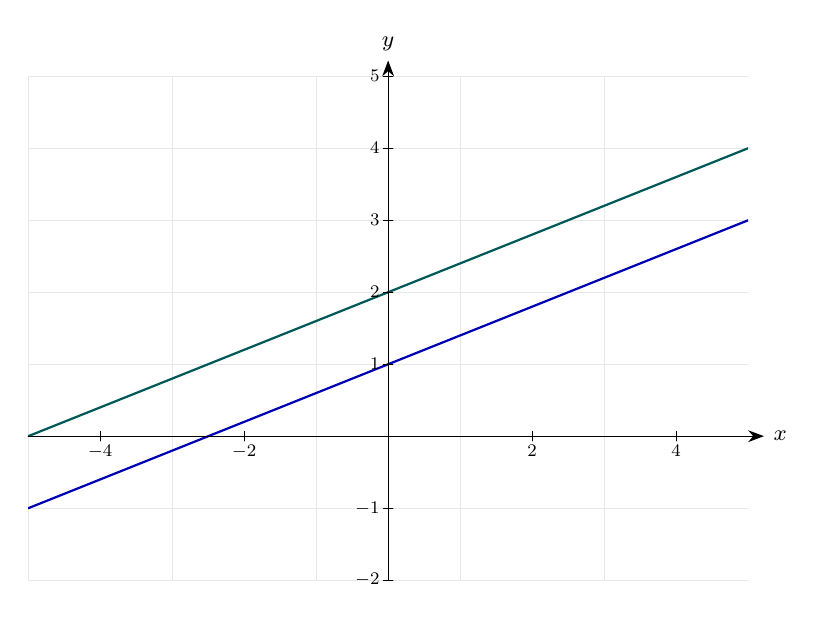
\begin{tikzpicture}[>={Stealth[length=2mm]},font=\footnotesize,line cap=round]
\begin{scope}
\clip (0,0) rectangle (9.143,6.4);
\draw[gray!18] (-0.914,0) grid[xstep=1.829,ystep=0.914] (9.143,6.4);
\draw[blue!70!black,thick] (0,0.914) -- (9.143,4.571);
\draw[teal!70!black,thick] (0,1.829) -- (9.143,5.486);
\end{scope}
\draw[->] (0,1.829) -- (9.343,1.829) node[right]{$x$};
\draw[->] (4.571,0) -- (4.571,6.6) node[above]{$y$};
\draw (0.914,1.769) -- (0.914,1.889) node[below=2pt,scale=0.8]{$-4$};
\draw (2.743,1.769) -- (2.743,1.889) node[below=2pt,scale=0.8]{$-2$};
\draw (6.4,1.769) -- (6.4,1.889) node[below=2pt,scale=0.8]{$2$};
\draw (8.229,1.769) -- (8.229,1.889) node[below=2pt,scale=0.8]{$4$};
\draw (4.511,0) -- (4.631,0) node[left=2pt,scale=0.8]{$-2$};
\draw (4.511,0.914) -- (4.631,0.914) node[left=2pt,scale=0.8]{$-1$};
\draw (4.511,2.743) -- (4.631,2.743) node[left=2pt,scale=0.8]{$1$};
\draw (4.511,3.657) -- (4.631,3.657) node[left=2pt,scale=0.8]{$2$};
\draw (4.511,4.571) -- (4.631,4.571) node[left=2pt,scale=0.8]{$3$};
\draw (4.511,5.486) -- (4.631,5.486) node[left=2pt,scale=0.8]{$4$};
\draw (4.511,6.4) -- (4.631,6.4) node[left=2pt,scale=0.8]{$5$};
\end{tikzpicture}
}
\end{center}
\small The line(s) and key points shown on the coordinate plane.\normalsize

\medskip\hrule

\section*{Parallel and Perpendicular Lines 39\quad\small\texttt{(cg3-039)}}
\addcontentsline{toc}{section}{Parallel and Perpendicular Lines 39 (cg3-039)}
\textit{Difficulty: Foundation \quad\textbar\quad Marks: 2}

\question{Find the value of \( k \) if the lines \( y = kx + 3 \) and \( y = -2x + 5 \) are perpendicular.}

\textbf{Worked solution.}

\textit{Product of gradients = -1}
\[\begin{gathered}
k \times (-2) = -1 \implies k = \frac{1}{2}
\end{gathered}\]
Perpendicular lines have gradients whose product is \( -1 \). Dividing both sides by \( -2 \) gives \( k = \tfrac{1}{2} \).

\begin{answerbox}
\textbf{Final answer:}\quad \(\displaystyle k = \frac{1}{2}\)
\end{answerbox}
\textbf{Diagram.}

\begin{center}
\resizebox{\ifdim\width>\linewidth \linewidth\else \width\fi}{!}{%
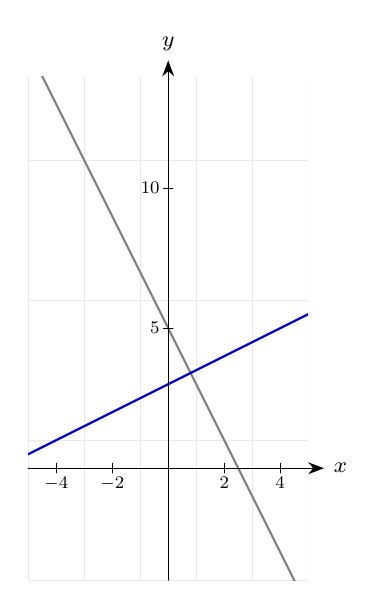
\begin{tikzpicture}[>={Stealth[length=2mm]},font=\footnotesize,line cap=round]
\begin{scope}
\clip (0,0) rectangle (3.556,6.4);
\draw[gray!18] (-0.356,-0.356) grid[xstep=0.711,ystep=1.778] (3.556,6.4);
\draw[gray,thick] (0,6.756) -- (3.556,-0.356);
\draw[blue!70!black,thick] (0,1.6) -- (3.556,3.378);
\end{scope}
\draw[->] (0,1.422) -- (3.756,1.422) node[right]{$x$};
\draw[->] (1.778,0) -- (1.778,6.6) node[above]{$y$};
\draw (0.356,1.362) -- (0.356,1.482) node[below=2pt,scale=0.8]{$-4$};
\draw (1.067,1.362) -- (1.067,1.482) node[below=2pt,scale=0.8]{$-2$};
\draw (2.489,1.362) -- (2.489,1.482) node[below=2pt,scale=0.8]{$2$};
\draw (3.2,1.362) -- (3.2,1.482) node[below=2pt,scale=0.8]{$4$};
\draw (1.718,3.2) -- (1.838,3.2) node[left=2pt,scale=0.8]{$5$};
\draw (1.718,4.978) -- (1.838,4.978) node[left=2pt,scale=0.8]{$10$};
\end{tikzpicture}
}
\end{center}
\small The line(s) and key points shown on the coordinate plane.\normalsize

\medskip\hrule

\section*{Parallel and Perpendicular Lines 40\quad\small\texttt{(cg3-040)}}
\addcontentsline{toc}{section}{Parallel and Perpendicular Lines 40 (cg3-040)}
\textit{Difficulty: Foundation \quad\textbar\quad Marks: 2}

\question{The line \( L_1 \) has equation \( 3x + 4y = 12 \). Find the equation of the line parallel to \( L_1 \) passing through the origin.}

\textbf{Worked solution.}

\textit{Step 1: Gradient of L1}
\[\begin{gathered}
4y = -3x + 12 \implies m = -\frac{3}{4}
\end{gathered}\]
Isolate \( y \) by subtracting \( 3x \) and dividing by \( 4 \). Coefficient of \( x \) is the gradient.

\textit{Step 2: Through origin}
\[\begin{gathered}
y = -\frac{3}{4}x
\end{gathered}\]
Through the origin, the \( y \)-intercept is \( 0 \), so \( c = 0 \).

\begin{answerbox}
\textbf{Final answer:}\quad \(\displaystyle y = -\frac{3}{4}x\)
\end{answerbox}
\textbf{Diagram.}

\begin{center}
\resizebox{\ifdim\width>\linewidth \linewidth\else \width\fi}{!}{%
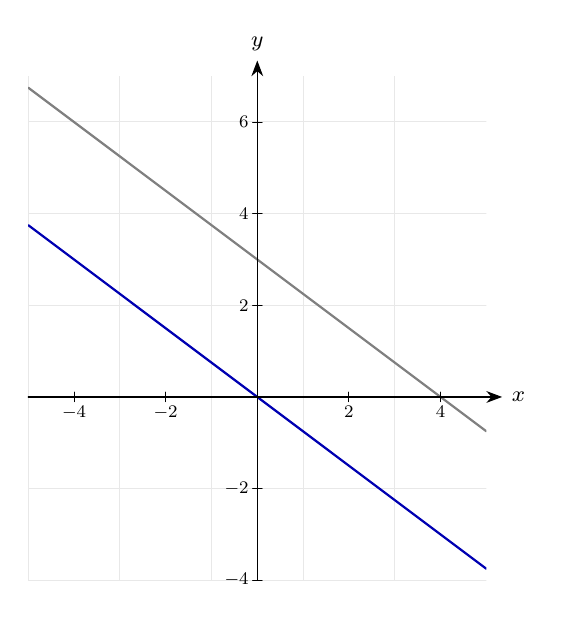
\begin{tikzpicture}[>={Stealth[length=2mm]},font=\footnotesize,line cap=round]
\begin{scope}
\clip (0,0) rectangle (5.818,6.4);
\draw[gray!18] (-0.582,0) grid[xstep=1.164,ystep=1.164] (5.818,6.4);
\draw[gray,thick] (0,6.255) -- (5.818,1.891);
\draw[blue!70!black,thick] (0,4.509) -- (5.818,0.145);
\end{scope}
\draw[->] (0,2.327) -- (6.018,2.327) node[right]{$x$};
\draw[->] (2.909,0) -- (2.909,6.6) node[above]{$y$};
\draw (0.582,2.267) -- (0.582,2.387) node[below=2pt,scale=0.8]{$-4$};
\draw (1.745,2.267) -- (1.745,2.387) node[below=2pt,scale=0.8]{$-2$};
\draw (4.073,2.267) -- (4.073,2.387) node[below=2pt,scale=0.8]{$2$};
\draw (5.236,2.267) -- (5.236,2.387) node[below=2pt,scale=0.8]{$4$};
\draw (2.849,0) -- (2.969,0) node[left=2pt,scale=0.8]{$-4$};
\draw (2.849,1.164) -- (2.969,1.164) node[left=2pt,scale=0.8]{$-2$};
\draw (2.849,3.491) -- (2.969,3.491) node[left=2pt,scale=0.8]{$2$};
\draw (2.849,4.655) -- (2.969,4.655) node[left=2pt,scale=0.8]{$4$};
\draw (2.849,5.818) -- (2.969,5.818) node[left=2pt,scale=0.8]{$6$};
\end{tikzpicture}
}
\end{center}
\small The line(s) and key points shown on the coordinate plane.\normalsize

\medskip\hrule

\section*{Parallel and Perpendicular Lines 41\quad\small\texttt{(cg3-041)}}
\addcontentsline{toc}{section}{Parallel and Perpendicular Lines 41 (cg3-041)}
\textit{Difficulty: Foundation \quad\textbar\quad Marks: 3}

\question{Find the equation of the line perpendicular to \( 2x - 5y + 10 = 0 \) passing through \( (4, -1) \).}

\textbf{Worked solution.}

\textit{Step 1: Gradient of given line}
\[\begin{gathered}
5y = 2x + 10 \implies m = \frac{2}{5}
\end{gathered}\]
Move \( -2x - 10 \) to the right and divide by \( 5 \) to read off the gradient.

\textit{Step 2: Perpendicular gradient and equation}
\[\begin{gathered}
m_{\perp} = -\frac{5}{2}; \quad y + 1 = -\frac{5}{2}(x - 4) \implies y = -\frac{5}{2}x + 9
\end{gathered}\]
Negative reciprocal of \( \tfrac{2}{5} \) is \( -\tfrac{5}{2} \). Expand: \( -\tfrac{5}{2}(x - 4) = -\tfrac{5}{2}x + 10 \), then subtract \( 1 \).

\begin{answerbox}
\textbf{Final answer:}\quad \(\displaystyle y = -\frac{5}{2}x + 9\)
\end{answerbox}
\textbf{Diagram.}

\begin{center}
\resizebox{\ifdim\width>\linewidth \linewidth\else \width\fi}{!}{%
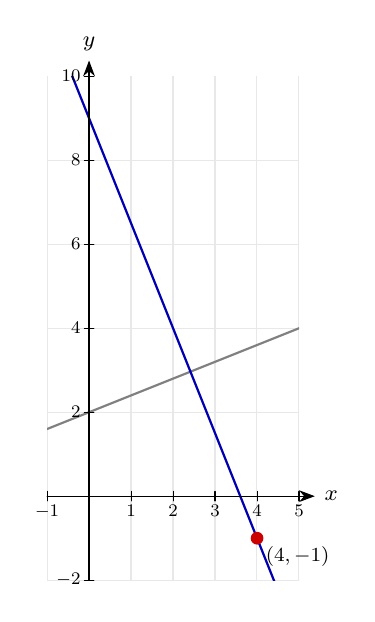
\begin{tikzpicture}[>={Stealth[length=2mm]},font=\footnotesize,line cap=round]
\begin{scope}
\clip (0,0) rectangle (3.2,6.4);
\draw[gray!18] (0,0) grid[xstep=0.533,ystep=1.067] (3.2,6.4);
\draw[gray,thick] (0,1.92) -- (3.2,3.2);
\draw[blue!70!black,thick] (0,7.2) -- (3.2,-0.8);
\end{scope}
\draw[->] (0,1.067) -- (3.4,1.067) node[right]{$x$};
\draw[->] (0.533,0) -- (0.533,6.6) node[above]{$y$};
\draw (0,1.007) -- (0,1.127) node[below=2pt,scale=0.8]{$-1$};
\draw (1.067,1.007) -- (1.067,1.127) node[below=2pt,scale=0.8]{$1$};
\draw (1.6,1.007) -- (1.6,1.127) node[below=2pt,scale=0.8]{$2$};
\draw (2.133,1.007) -- (2.133,1.127) node[below=2pt,scale=0.8]{$3$};
\draw (2.667,1.007) -- (2.667,1.127) node[below=2pt,scale=0.8]{$4$};
\draw (3.2,1.007) -- (3.2,1.127) node[below=2pt,scale=0.8]{$5$};
\draw (0.473,0) -- (0.593,0) node[left=2pt,scale=0.8]{$-2$};
\draw (0.473,2.133) -- (0.593,2.133) node[left=2pt,scale=0.8]{$2$};
\draw (0.473,3.2) -- (0.593,3.2) node[left=2pt,scale=0.8]{$4$};
\draw (0.473,4.267) -- (0.593,4.267) node[left=2pt,scale=0.8]{$6$};
\draw (0.473,5.333) -- (0.593,5.333) node[left=2pt,scale=0.8]{$8$};
\draw (0.473,6.4) -- (0.593,6.4) node[left=2pt,scale=0.8]{$10$};
\fill[red!80!black] (2.667,0.533) circle (2.3pt);
\node[below right,scale=0.9] at (2.667,0.533) {$(4,-1)$};
\end{tikzpicture}
}
\end{center}
\small The line(s) and key points shown on the coordinate plane.\normalsize

\medskip\hrule

\section*{Parallel and Perpendicular Lines 42\quad\small\texttt{(cg3-042)}}
\addcontentsline{toc}{section}{Parallel and Perpendicular Lines 42 (cg3-042)}
\textit{Difficulty: Foundation \quad\textbar\quad Marks: 2}

\question{Show that the lines \( y = 5x - 3 \) and \( x + 5y = 20 \) are perpendicular.}

\textbf{Worked solution.}

\textit{Find gradients and check product}
\[\begin{gathered}
m_1 = 5; \quad 5y = -x + 20 \implies m_2 = -\frac{1}{5}; \quad 5 \times (-\frac{1}{5}) = -1 \checkmark
\end{gathered}\]
The first line is already in \( y = mx + c \) form. Rearrange the second by dividing by \( 5 \). The product of the gradients is \( -1 \), confirming perpendicularity.

\begin{answerbox}
\textbf{Final answer:}\quad Product of gradients is \(\displaystyle -1\), so perpendicular.
\end{answerbox}
\textbf{Diagram.}

\begin{center}
\resizebox{\ifdim\width>\linewidth \linewidth\else \width\fi}{!}{%
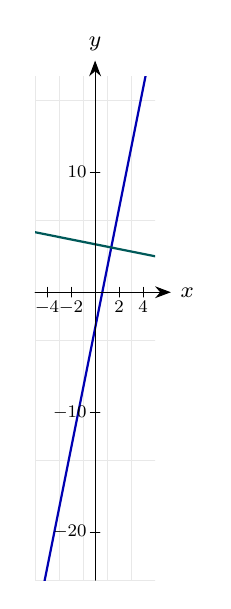
\begin{tikzpicture}[>={Stealth[length=2mm]},font=\footnotesize,line cap=round]
\begin{scope}
\clip (0,0) rectangle (1.524,6.4);
\draw[gray!18] (-0.152,-0.914) grid[xstep=0.305,ystep=1.524] (1.524,6.4);
\draw[blue!70!black,thick] (0,-0.61) -- (1.524,7.01);
\draw[teal!70!black,thick] (0,4.419) -- (1.524,4.114);
\end{scope}
\draw[->] (0,3.657) -- (1.724,3.657) node[right]{$x$};
\draw[->] (0.762,0) -- (0.762,6.6) node[above]{$y$};
\draw (0.152,3.597) -- (0.152,3.717) node[below=2pt,scale=0.8]{$-4$};
\draw (0.457,3.597) -- (0.457,3.717) node[below=2pt,scale=0.8]{$-2$};
\draw (1.067,3.597) -- (1.067,3.717) node[below=2pt,scale=0.8]{$2$};
\draw (1.371,3.597) -- (1.371,3.717) node[below=2pt,scale=0.8]{$4$};
\draw (0.702,0.61) -- (0.822,0.61) node[left=2pt,scale=0.8]{$-20$};
\draw (0.702,2.133) -- (0.822,2.133) node[left=2pt,scale=0.8]{$-10$};
\draw (0.702,5.181) -- (0.822,5.181) node[left=2pt,scale=0.8]{$10$};
\end{tikzpicture}
}
\end{center}
\small The line(s) and key points shown on the coordinate plane.\normalsize

\medskip\hrule

\section*{Parallel and Perpendicular Lines 43\quad\small\texttt{(cg3-043)}}
\addcontentsline{toc}{section}{Parallel and Perpendicular Lines 43 (cg3-043)}
\textit{Difficulty: Foundation \quad\textbar\quad Marks: 3}

\question{Find the value of \( p \) such that the lines \( px + 3y = 6 \) and \( 2x - y = 4 \) are parallel.}

\textbf{Worked solution.}

\textit{Step 1: Gradients}
\[\begin{gathered}
m_1 = -\frac{p}{3}; \quad m_2 = 2
\end{gathered}\]
From \( px + 3y = 6 \): \( 3y = -px + 6 \), so \( m_1 = -\tfrac{p}{3} \). From \( 2x - y = 4 \): \( y = 2x - 4 \), so \( m_2 = 2 \).

\textit{Step 2: Set equal for parallel}
\[\begin{gathered}
-\frac{p}{3} = 2 \implies p = -6
\end{gathered}\]
Multiply both sides by \( -3 \); the sign flips, giving \( p = -6 \).

\begin{answerbox}
\textbf{Final answer:}\quad \(\displaystyle p = -6\)
\end{answerbox}
\textbf{Diagram.}

\begin{center}
\resizebox{\ifdim\width>\linewidth \linewidth\else \width\fi}{!}{%
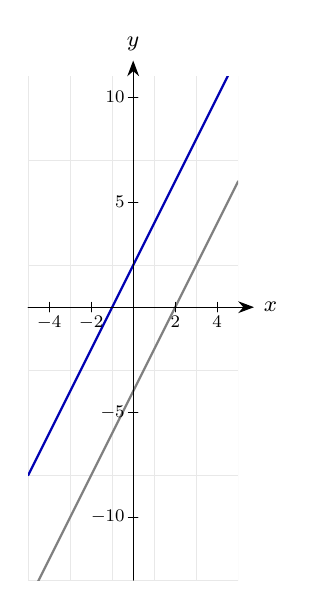
\begin{tikzpicture}[>={Stealth[length=2mm]},font=\footnotesize,line cap=round]
\begin{scope}
\clip (0,0) rectangle (2.667,6.4);
\draw[gray!18] (-0.267,-0.533) grid[xstep=0.533,ystep=1.333] (2.667,6.4);
\draw[gray,thick] (0,-0.267) -- (2.667,5.067);
\draw[blue!70!black,thick] (0,1.333) -- (2.667,6.667);
\end{scope}
\draw[->] (0,3.467) -- (2.867,3.467) node[right]{$x$};
\draw[->] (1.333,0) -- (1.333,6.6) node[above]{$y$};
\draw (0.267,3.407) -- (0.267,3.527) node[below=2pt,scale=0.8]{$-4$};
\draw (0.8,3.407) -- (0.8,3.527) node[below=2pt,scale=0.8]{$-2$};
\draw (1.867,3.407) -- (1.867,3.527) node[below=2pt,scale=0.8]{$2$};
\draw (2.4,3.407) -- (2.4,3.527) node[below=2pt,scale=0.8]{$4$};
\draw (1.273,0.8) -- (1.393,0.8) node[left=2pt,scale=0.8]{$-10$};
\draw (1.273,2.133) -- (1.393,2.133) node[left=2pt,scale=0.8]{$-5$};
\draw (1.273,4.8) -- (1.393,4.8) node[left=2pt,scale=0.8]{$5$};
\draw (1.273,6.133) -- (1.393,6.133) node[left=2pt,scale=0.8]{$10$};
\end{tikzpicture}
}
\end{center}
\small The line(s) and key points shown on the coordinate plane.\normalsize

\medskip\hrule

\section*{Parallel and Perpendicular Lines 44\quad\small\texttt{(cg3-044)}}
\addcontentsline{toc}{section}{Parallel and Perpendicular Lines 44 (cg3-044)}
\textit{Difficulty: Foundation \quad\textbar\quad Marks: 4}

\question{The line \( L \) passes through \( A(1, 5) \) and \( B(3, -1) \). Find the equation of the line through \( (4, 2) \) perpendicular to \( L \).}

\textbf{Worked solution.}

\textit{Step 1: Gradient of L}
\[\begin{gathered}
m_L = \frac{-1-5}{3-1} = -3
\end{gathered}\]
Apply the gradient formula to \( A \) and \( B \): \( \tfrac{-6}{2} = -3 \).

\textit{Step 2: Perpendicular and equation}
\[\begin{gathered}
m_{\perp} = \frac{1}{3}; \quad y - 2 = \frac{1}{3}(x - 4) \implies y = \frac{1}{3}x + \frac{2}{3}
\end{gathered}\]
Negative reciprocal of \( -3 \) is \( \tfrac{1}{3} \). Expand: \( \tfrac{1}{3}(x - 4) = \tfrac{1}{3}x - \tfrac{4}{3} \), then add \( 2 = \tfrac{6}{3} \) to get \( +\tfrac{2}{3} \).

\begin{answerbox}
\textbf{Final answer:}\quad \(\displaystyle y = \frac{1}{3}x + \frac{2}{3}\)
\end{answerbox}
\textbf{Diagram.}

\begin{center}
\resizebox{\ifdim\width>\linewidth \linewidth\else \width\fi}{!}{%
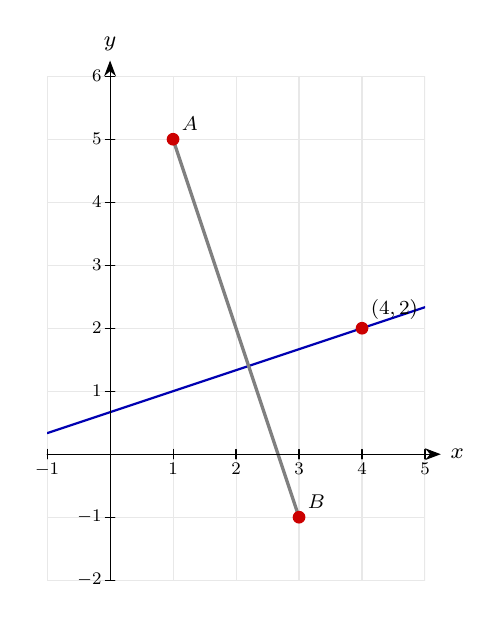
\begin{tikzpicture}[>={Stealth[length=2mm]},font=\footnotesize,line cap=round]
\begin{scope}
\clip (0,0) rectangle (4.8,6.4);
\draw[gray!18] (0,0) grid[xstep=0.8,ystep=0.8] (4.8,6.4);
\draw[blue!70!black,thick] (0,1.867) -- (4.8,3.467);
\draw[gray,very thick] (1.6,5.6) -- (3.2,0.8);
\end{scope}
\draw[->] (0,1.6) -- (5,1.6) node[right]{$x$};
\draw[->] (0.8,0) -- (0.8,6.6) node[above]{$y$};
\draw (0,1.54) -- (0,1.66) node[below=2pt,scale=0.8]{$-1$};
\draw (1.6,1.54) -- (1.6,1.66) node[below=2pt,scale=0.8]{$1$};
\draw (2.4,1.54) -- (2.4,1.66) node[below=2pt,scale=0.8]{$2$};
\draw (3.2,1.54) -- (3.2,1.66) node[below=2pt,scale=0.8]{$3$};
\draw (4,1.54) -- (4,1.66) node[below=2pt,scale=0.8]{$4$};
\draw (4.8,1.54) -- (4.8,1.66) node[below=2pt,scale=0.8]{$5$};
\draw (0.74,0) -- (0.86,0) node[left=2pt,scale=0.8]{$-2$};
\draw (0.74,0.8) -- (0.86,0.8) node[left=2pt,scale=0.8]{$-1$};
\draw (0.74,2.4) -- (0.86,2.4) node[left=2pt,scale=0.8]{$1$};
\draw (0.74,3.2) -- (0.86,3.2) node[left=2pt,scale=0.8]{$2$};
\draw (0.74,4) -- (0.86,4) node[left=2pt,scale=0.8]{$3$};
\draw (0.74,4.8) -- (0.86,4.8) node[left=2pt,scale=0.8]{$4$};
\draw (0.74,5.6) -- (0.86,5.6) node[left=2pt,scale=0.8]{$5$};
\draw (0.74,6.4) -- (0.86,6.4) node[left=2pt,scale=0.8]{$6$};
\fill[red!80!black] (1.6,5.6) circle (2.3pt);
\node[above right,scale=0.9] at (1.6,5.6) {$A$};
\fill[red!80!black] (3.2,0.8) circle (2.3pt);
\node[above right,scale=0.9] at (3.2,0.8) {$B$};
\fill[red!80!black] (4,3.2) circle (2.3pt);
\node[above right,scale=0.9] at (4,3.2) {$(4,2)$};
\end{tikzpicture}
}
\end{center}
\small The line(s) and key points shown on the coordinate plane.\normalsize

\medskip\hrule

\section*{Parallel and Perpendicular Lines 45\quad\small\texttt{(cg3-045)}}
\addcontentsline{toc}{section}{Parallel and Perpendicular Lines 45 (cg3-045)}
\textit{Difficulty: Foundation \quad\textbar\quad Marks: 5}

\question{Find the foot of the perpendicular from \( P(3, 7) \) to the line \( y = 2x + 1 \).}

\textbf{Worked solution.}

\textit{Step 1: Perpendicular from P has gradient -1/2}
\[\begin{gathered}
y - 7 = -\frac{1}{2}(x - 3) \implies y = -\frac{1}{2}x + \frac{17}{2}
\end{gathered}\]
The perpendicular gradient is the negative reciprocal of \( 2 \). Use point-slope form through \( P(3, 7) \).

\textit{Step 2: Solve simultaneously}
\[\begin{gathered}
2x + 1 = -\frac{1}{2}x + \frac{17}{2} \implies \frac{5}{2}x = \frac{15}{2} \implies x = 3,\ y = 7
\end{gathered}\]
Setting the two equations equal finds their intersection. Quick check: \( y = 2(3) + 1 = 7 \), so \( P \) itself lies on the line --- the foot of the perpendicular from a point on the line is that point.

\begin{answerbox}
\textbf{Final answer:}\quad \(\displaystyle P(3, 7)\) lies on the line, so the foot of the perpendicular is \(\displaystyle P\) itself.
\end{answerbox}
\textbf{Diagram.}

\begin{center}
\resizebox{\ifdim\width>\linewidth \linewidth\else \width\fi}{!}{%
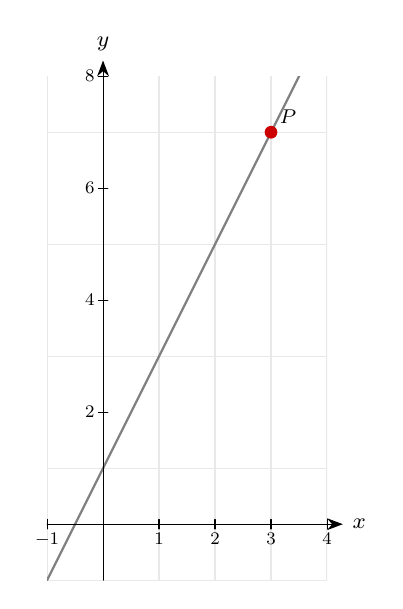
\begin{tikzpicture}[>={Stealth[length=2mm]},font=\footnotesize,line cap=round]
\begin{scope}
\clip (0,0) rectangle (3.556,6.4);
\draw[gray!18] (0,-0.711) grid[xstep=0.711,ystep=1.422] (3.556,6.4);
\draw[gray,thick] (0,0) -- (3.556,7.111);
\end{scope}
\draw[->] (0,0.711) -- (3.756,0.711) node[right]{$x$};
\draw[->] (0.711,0) -- (0.711,6.6) node[above]{$y$};
\draw (0,0.651) -- (0,0.771) node[below=2pt,scale=0.8]{$-1$};
\draw (1.422,0.651) -- (1.422,0.771) node[below=2pt,scale=0.8]{$1$};
\draw (2.133,0.651) -- (2.133,0.771) node[below=2pt,scale=0.8]{$2$};
\draw (2.844,0.651) -- (2.844,0.771) node[below=2pt,scale=0.8]{$3$};
\draw (3.556,0.651) -- (3.556,0.771) node[below=2pt,scale=0.8]{$4$};
\draw (0.651,2.133) -- (0.771,2.133) node[left=2pt,scale=0.8]{$2$};
\draw (0.651,3.556) -- (0.771,3.556) node[left=2pt,scale=0.8]{$4$};
\draw (0.651,4.978) -- (0.771,4.978) node[left=2pt,scale=0.8]{$6$};
\draw (0.651,6.4) -- (0.771,6.4) node[left=2pt,scale=0.8]{$8$};
\fill[red!80!black] (2.844,5.689) circle (2.3pt);
\node[above right,scale=0.9] at (2.844,5.689) {$P$};
\end{tikzpicture}
}
\end{center}
\small The line(s) and key points shown on the coordinate plane.\normalsize

\medskip\hrule

\section*{Parallel and Perpendicular Lines 46\quad\small\texttt{(cg3-046)}}
\addcontentsline{toc}{section}{Parallel and Perpendicular Lines 46 (cg3-046)}
\textit{Difficulty: Foundation \quad\textbar\quad Marks: 4}

\question{Find the foot of the perpendicular from \( P(4, 5) \) to the line \( y = x + 1 \).}

\textbf{Worked solution.}

\textit{Step 1: Perpendicular from P}
\[\begin{gathered}
m_{\perp} = -1; \quad y - 5 = -(x - 4) \implies y = -x + 9
\end{gathered}\]
The line \( y = x + 1 \) has gradient \( 1 \), so the perpendicular has gradient \( -1 \). Point-slope form through \( P(4, 5) \).

\textit{Step 2: Solve with y = x + 1}
\[\begin{gathered}
x + 1 = -x + 9 \implies 2x = 8 \implies x = 4,\ y = 5
\end{gathered}\]
Setting the equations equal gives the foot of the perpendicular. Note that \( P(4, 5) \) satisfies \( y = x + 1 \), so \( P \) lies on the line and the foot is \( P \) itself.

\begin{answerbox}
\textbf{Final answer:}\quad \(\displaystyle (4, 5)\)
\end{answerbox}
\textbf{Diagram.}

\begin{center}
\resizebox{\ifdim\width>\linewidth \linewidth\else \width\fi}{!}{%
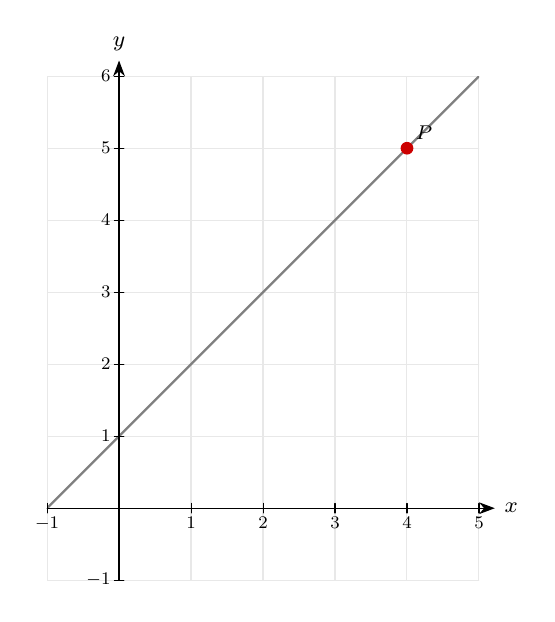
\begin{tikzpicture}[>={Stealth[length=2mm]},font=\footnotesize,line cap=round]
\begin{scope}
\clip (0,0) rectangle (5.486,6.4);
\draw[gray!18] (0,0) grid[xstep=0.914,ystep=0.914] (5.486,6.4);
\draw[gray,thick] (0,0.914) -- (5.486,6.4);
\end{scope}
\draw[->] (0,0.914) -- (5.686,0.914) node[right]{$x$};
\draw[->] (0.914,0) -- (0.914,6.6) node[above]{$y$};
\draw (0,0.854) -- (0,0.974) node[below=2pt,scale=0.8]{$-1$};
\draw (1.829,0.854) -- (1.829,0.974) node[below=2pt,scale=0.8]{$1$};
\draw (2.743,0.854) -- (2.743,0.974) node[below=2pt,scale=0.8]{$2$};
\draw (3.657,0.854) -- (3.657,0.974) node[below=2pt,scale=0.8]{$3$};
\draw (4.571,0.854) -- (4.571,0.974) node[below=2pt,scale=0.8]{$4$};
\draw (5.486,0.854) -- (5.486,0.974) node[below=2pt,scale=0.8]{$5$};
\draw (0.854,0) -- (0.974,0) node[left=2pt,scale=0.8]{$-1$};
\draw (0.854,1.829) -- (0.974,1.829) node[left=2pt,scale=0.8]{$1$};
\draw (0.854,2.743) -- (0.974,2.743) node[left=2pt,scale=0.8]{$2$};
\draw (0.854,3.657) -- (0.974,3.657) node[left=2pt,scale=0.8]{$3$};
\draw (0.854,4.571) -- (0.974,4.571) node[left=2pt,scale=0.8]{$4$};
\draw (0.854,5.486) -- (0.974,5.486) node[left=2pt,scale=0.8]{$5$};
\draw (0.854,6.4) -- (0.974,6.4) node[left=2pt,scale=0.8]{$6$};
\fill[red!80!black] (4.571,5.486) circle (2.3pt);
\node[above right,scale=0.9] at (4.571,5.486) {$P$};
\end{tikzpicture}
}
\end{center}
\small The line(s) and key points shown on the coordinate plane.\normalsize

\medskip\hrule

\section*{Parallel and Perpendicular Lines 47\quad\small\texttt{(cg3-047)}}
\addcontentsline{toc}{section}{Parallel and Perpendicular Lines 47 (cg3-047)}
\textit{Difficulty: Foundation \quad\textbar\quad Marks: 4}

\question{Find the foot of the perpendicular from \( P(1, 6) \) to the line \( y = 3x - 2 \).}

\textbf{Worked solution.}

\textit{Step 1: Perpendicular from P}
\[\begin{gathered}
m_{\perp} = -\frac{1}{3}; \quad y - 6 = -\frac{1}{3}(x - 1) \implies y = -\frac{1}{3}x + \frac{19}{3}
\end{gathered}\]
Negative reciprocal of \( 3 \). Expand and add: \( \tfrac{1}{3} + 6 = \tfrac{1}{3} + \tfrac{18}{3} = \tfrac{19}{3} \).

\textit{Step 2: Solve simultaneously}
\[\begin{gathered}
3x - 2 = -\frac{1}{3}x + \frac{19}{3} \implies \frac{10}{3}x = \frac{25}{3} \implies x = \frac{5}{2}, y = \frac{11}{2}
\end{gathered}\]
Add \( \tfrac{1}{3}x \) to both sides: \( 3x + \tfrac{1}{3}x = \tfrac{10}{3}x \). Then \( \tfrac{25}{3} \div \tfrac{10}{3} = \tfrac{5}{2} \). Substitute back into \( y = 3x - 2 \) to get \( y = \tfrac{15}{2} - 2 = \tfrac{11}{2} \).

\begin{answerbox}
\textbf{Final answer:}\quad \(\displaystyle \left(\frac{5}{2}, \frac{11}{2}\right)\)
\end{answerbox}
\textbf{Diagram.}

\begin{center}
\resizebox{\ifdim\width>\linewidth \linewidth\else \width\fi}{!}{%
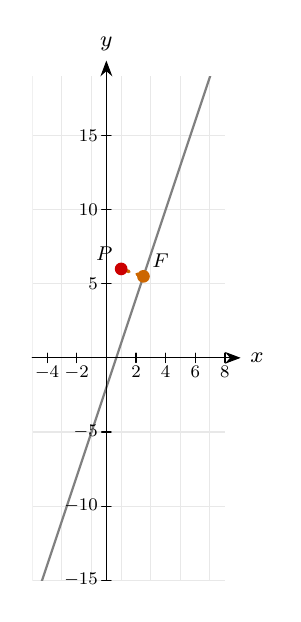
\begin{tikzpicture}[>={Stealth[length=2mm]},font=\footnotesize,line cap=round]
\begin{scope}
\clip (0,0) rectangle (2.447,6.4);
\draw[gray!18] (-0.188,0) grid[xstep=0.376,ystep=0.941] (2.447,6.4);
\draw[gray,thick] (0,-0.376) -- (2.447,6.965);
\draw[dashed,orange!80!black,very thick] (1.129,3.953) -- (1.412,3.859);
\end{scope}
\draw[->] (0,2.824) -- (2.647,2.824) node[right]{$x$};
\draw[->] (0.941,0) -- (0.941,6.6) node[above]{$y$};
\draw (0.188,2.764) -- (0.188,2.884) node[below=2pt,scale=0.8]{$-4$};
\draw (0.565,2.764) -- (0.565,2.884) node[below=2pt,scale=0.8]{$-2$};
\draw (1.318,2.764) -- (1.318,2.884) node[below=2pt,scale=0.8]{$2$};
\draw (1.694,2.764) -- (1.694,2.884) node[below=2pt,scale=0.8]{$4$};
\draw (2.071,2.764) -- (2.071,2.884) node[below=2pt,scale=0.8]{$6$};
\draw (2.447,2.764) -- (2.447,2.884) node[below=2pt,scale=0.8]{$8$};
\draw (0.881,0) -- (1.001,0) node[left=2pt,scale=0.8]{$-15$};
\draw (0.881,0.941) -- (1.001,0.941) node[left=2pt,scale=0.8]{$-10$};
\draw (0.881,1.882) -- (1.001,1.882) node[left=2pt,scale=0.8]{$-5$};
\draw (0.881,3.765) -- (1.001,3.765) node[left=2pt,scale=0.8]{$5$};
\draw (0.881,4.706) -- (1.001,4.706) node[left=2pt,scale=0.8]{$10$};
\draw (0.881,5.647) -- (1.001,5.647) node[left=2pt,scale=0.8]{$15$};
\fill[red!80!black] (1.129,3.953) circle (2.3pt);
\node[above left,scale=0.9] at (1.129,3.953) {$P$};
\fill[orange!80!black] (1.412,3.859) circle (2.3pt);
\node[above right,scale=0.9] at (1.412,3.859) {$F$};
\end{tikzpicture}
}
\end{center}
\small The line(s) and key points shown on the coordinate plane.\normalsize

\medskip\hrule

\section*{Parallel and Perpendicular Lines 48\quad\small\texttt{(cg3-048)}}
\addcontentsline{toc}{section}{Parallel and Perpendicular Lines 48 (cg3-048)}
\textit{Difficulty: Foundation \quad\textbar\quad Marks: 4}

\question{The line \( L_1: y = -\frac{3}{4}x + 6 \) meets the x-axis at \( A \). Find the equation of the line through \( A \) perpendicular to \( L_1 \).}

\textbf{Worked solution.}

\textit{Step 1: Find A (y = 0)}
\[\begin{gathered}
0 = -\frac{3}{4}x + 6 \implies x = 8, \quad A = (8, 0)
\end{gathered}\]
At the \( x \)-axis, \( y = 0 \). Solve for \( x \): \( \tfrac{3}{4}x = 6 \), so \( x = 8 \).

\textit{Step 2: Perpendicular gradient and equation}
\[\begin{gathered}
m_{\perp} = \frac{4}{3}; \quad y = \frac{4}{3}(x - 8) = \frac{4}{3}x - \frac{32}{3}
\end{gathered}\]
Negative reciprocal of \( -\tfrac{3}{4} \) is \( \tfrac{4}{3} \). Since the line passes through \( A(8, 0) \), use point-slope with \( y_1 = 0 \).

\begin{answerbox}
\textbf{Final answer:}\quad \(\displaystyle y = \frac{4}{3}x - \frac{32}{3}\)
\end{answerbox}
\textbf{Diagram.}

\begin{center}
\resizebox{\ifdim\width>\linewidth \linewidth\else \width\fi}{!}{%
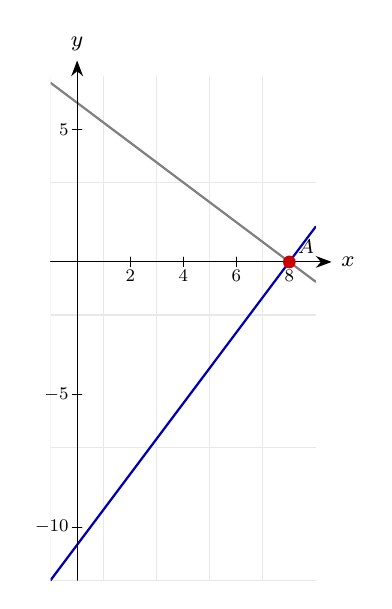
\begin{tikzpicture}[>={Stealth[length=2mm]},font=\footnotesize,line cap=round]
\begin{scope}
\clip (0,0) rectangle (3.368,6.4);
\draw[gray!18] (-0.337,-1.011) grid[xstep=0.674,ystep=1.684] (3.368,6.4);
\draw[gray,thick] (0,6.316) -- (3.368,3.789);
\draw[blue!70!black,thick] (0,0) -- (3.368,4.491);
\end{scope}
\draw[->] (0,4.042) -- (3.568,4.042) node[right]{$x$};
\draw[->] (0.337,0) -- (0.337,6.6) node[above]{$y$};
\draw (1.011,3.982) -- (1.011,4.102) node[below=2pt,scale=0.8]{$2$};
\draw (1.684,3.982) -- (1.684,4.102) node[below=2pt,scale=0.8]{$4$};
\draw (2.358,3.982) -- (2.358,4.102) node[below=2pt,scale=0.8]{$6$};
\draw (3.032,3.982) -- (3.032,4.102) node[below=2pt,scale=0.8]{$8$};
\draw (0.277,0.674) -- (0.397,0.674) node[left=2pt,scale=0.8]{$-10$};
\draw (0.277,2.358) -- (0.397,2.358) node[left=2pt,scale=0.8]{$-5$};
\draw (0.277,5.726) -- (0.397,5.726) node[left=2pt,scale=0.8]{$5$};
\fill[red!80!black] (3.032,4.042) circle (2.3pt);
\node[above right,scale=0.9] at (3.032,4.042) {$A$};
\end{tikzpicture}
}
\end{center}
\small The line(s) and key points shown on the coordinate plane.\normalsize

\medskip\hrule

\section*{Parallel and Perpendicular Lines 49\quad\small\texttt{(cg3-049)}}
\addcontentsline{toc}{section}{Parallel and Perpendicular Lines 49 (cg3-049)}
\textit{Difficulty: Foundation \quad\textbar\quad Marks: 3}

\question{Find the values of \( k \) for which \( kx + 2y = 5 \) is perpendicular to \( 3x - 4y = 1 \).}

\textbf{Worked solution.}

\textit{Step 1: Gradients}
\[\begin{gathered}
m_1 = -\frac{k}{2}; \quad m_2 = \frac{3}{4}
\end{gathered}\]
From \( kx + 2y = 5 \): \( y = -\tfrac{k}{2}x + \tfrac{5}{2} \). From \( 3x - 4y = 1 \): \( 4y = 3x - 1 \), so \( m_2 = \tfrac{3}{4} \).

\textit{Step 2: Product = -1}
\[\begin{gathered}
-\frac{k}{2} \times \frac{3}{4} = -1 \implies \frac{3k}{8} = 1 \implies k = \frac{8}{3}
\end{gathered}\]
Multiplying gives \( -\tfrac{3k}{8} = -1 \), so \( \tfrac{3k}{8} = 1 \). Multiply both sides by \( \tfrac{8}{3} \).

\begin{answerbox}
\textbf{Final answer:}\quad \(\displaystyle k = \frac{8}{3}\)
\end{answerbox}
\textbf{Diagram.}

\begin{center}
\resizebox{\ifdim\width>\linewidth \linewidth\else \width\fi}{!}{%
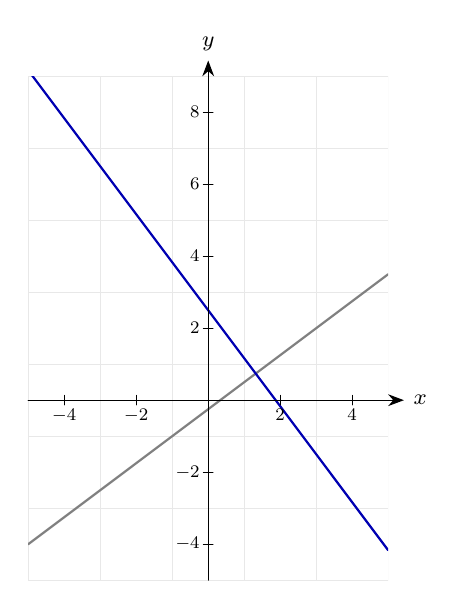
\begin{tikzpicture}[>={Stealth[length=2mm]},font=\footnotesize,line cap=round]
\begin{scope}
\clip (0,0) rectangle (4.571,6.4);
\draw[gray!18] (-0.457,-0.457) grid[xstep=0.914,ystep=0.914] (4.571,6.4);
\draw[gray,thick] (0,0.457) -- (4.571,3.886);
\draw[blue!70!black,thick] (0,6.476) -- (4.571,0.381);
\end{scope}
\draw[->] (0,2.286) -- (4.771,2.286) node[right]{$x$};
\draw[->] (2.286,0) -- (2.286,6.6) node[above]{$y$};
\draw (0.457,2.226) -- (0.457,2.346) node[below=2pt,scale=0.8]{$-4$};
\draw (1.371,2.226) -- (1.371,2.346) node[below=2pt,scale=0.8]{$-2$};
\draw (3.2,2.226) -- (3.2,2.346) node[below=2pt,scale=0.8]{$2$};
\draw (4.114,2.226) -- (4.114,2.346) node[below=2pt,scale=0.8]{$4$};
\draw (2.226,0.457) -- (2.346,0.457) node[left=2pt,scale=0.8]{$-4$};
\draw (2.226,1.371) -- (2.346,1.371) node[left=2pt,scale=0.8]{$-2$};
\draw (2.226,3.2) -- (2.346,3.2) node[left=2pt,scale=0.8]{$2$};
\draw (2.226,4.114) -- (2.346,4.114) node[left=2pt,scale=0.8]{$4$};
\draw (2.226,5.029) -- (2.346,5.029) node[left=2pt,scale=0.8]{$6$};
\draw (2.226,5.943) -- (2.346,5.943) node[left=2pt,scale=0.8]{$8$};
\end{tikzpicture}
}
\end{center}
\small The line(s) and key points shown on the coordinate plane.\normalsize

\medskip\hrule

\section*{Parallel and Perpendicular Lines 50\quad\small\texttt{(cg3-050)}}
\addcontentsline{toc}{section}{Parallel and Perpendicular Lines 50 (cg3-050)}
\textit{Difficulty: Foundation \quad\textbar\quad Marks: 3}

\question{A triangle has vertices \( A(0, 0) \), \( B(6, 0) \), \( C(2, 4) \). Find the equation of the altitude from \( C \) to \( AB \).}

\textbf{Worked solution.}

\textit{Step 1: AB is horizontal (y = 0)}
\[\begin{gathered}
m_{AB} = 0
\end{gathered}\]
Both \( A \) and \( B \) have \( y = 0 \), so \( AB \) lies along the \( x \)-axis.

\textit{Step 2: Altitude from C is vertical}
\[\begin{gathered}
x = 2
\end{gathered}\]
Perpendicular to a horizontal line is vertical.

\begin{answerbox}
\textbf{Final answer:}\quad \(\displaystyle x = 2\)
\end{answerbox}
\textbf{Diagram.}

\begin{center}
\resizebox{\ifdim\width>\linewidth \linewidth\else \width\fi}{!}{%
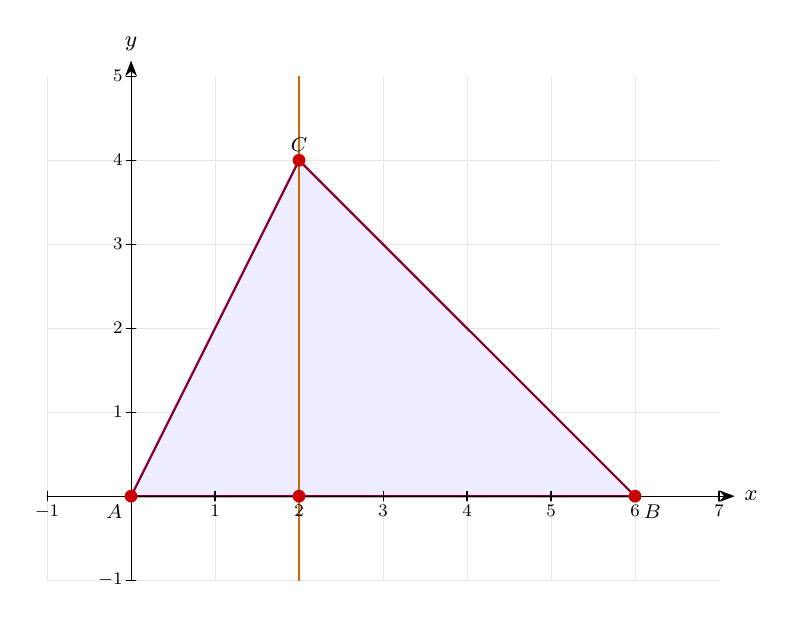
\begin{tikzpicture}[>={Stealth[length=2mm]},font=\footnotesize,line cap=round]
\begin{scope}
\clip (0,0) rectangle (8.533,6.4);
\draw[gray!18] (0,0) grid[xstep=1.067,ystep=1.067] (8.533,6.4);
\fill[blue!7] (1.067,1.067) -- (7.467,1.067) -- (3.2,5.333) -- cycle;
\draw[purple!70!black,thick] (1.067,1.067) -- (7.467,1.067) -- (3.2,5.333) -- cycle;
\draw[orange!80!black,thick] (3.2,0) -- (3.2,6.4);
\end{scope}
\draw[->] (0,1.067) -- (8.733,1.067) node[right]{$x$};
\draw[->] (1.067,0) -- (1.067,6.6) node[above]{$y$};
\draw (0,1.007) -- (0,1.127) node[below=2pt,scale=0.8]{$-1$};
\draw (2.133,1.007) -- (2.133,1.127) node[below=2pt,scale=0.8]{$1$};
\draw (3.2,1.007) -- (3.2,1.127) node[below=2pt,scale=0.8]{$2$};
\draw (4.267,1.007) -- (4.267,1.127) node[below=2pt,scale=0.8]{$3$};
\draw (5.333,1.007) -- (5.333,1.127) node[below=2pt,scale=0.8]{$4$};
\draw (6.4,1.007) -- (6.4,1.127) node[below=2pt,scale=0.8]{$5$};
\draw (7.467,1.007) -- (7.467,1.127) node[below=2pt,scale=0.8]{$6$};
\draw (8.533,1.007) -- (8.533,1.127) node[below=2pt,scale=0.8]{$7$};
\draw (1.007,0) -- (1.127,0) node[left=2pt,scale=0.8]{$-1$};
\draw (1.007,2.133) -- (1.127,2.133) node[left=2pt,scale=0.8]{$1$};
\draw (1.007,3.2) -- (1.127,3.2) node[left=2pt,scale=0.8]{$2$};
\draw (1.007,4.267) -- (1.127,4.267) node[left=2pt,scale=0.8]{$3$};
\draw (1.007,5.333) -- (1.127,5.333) node[left=2pt,scale=0.8]{$4$};
\draw (1.007,6.4) -- (1.127,6.4) node[left=2pt,scale=0.8]{$5$};
\fill[red!80!black] (1.067,1.067) circle (2.3pt);
\node[below left,scale=0.9] at (1.067,1.067) {$A$};
\fill[red!80!black] (7.467,1.067) circle (2.3pt);
\node[below right,scale=0.9] at (7.467,1.067) {$B$};
\fill[red!80!black] (3.2,5.333) circle (2.3pt);
\node[above,scale=0.9] at (3.2,5.333) {$C$};
\fill[red!80!black] (3.2,1.067) circle (2.3pt);
\end{tikzpicture}
}
\end{center}
\small The line(s) and key points shown on the coordinate plane.\normalsize

\medskip\hrule

\section*{Parallel and Perpendicular Lines 51\quad\small\texttt{(cg3-051)}}
\addcontentsline{toc}{section}{Parallel and Perpendicular Lines 51 (cg3-051)}
\textit{Difficulty: Foundation \quad\textbar\quad Marks: 4}

\question{Find the equation of the altitude from \( A(0, 0) \) to \( BC \) where \( B(6, 0) \) and \( C(2, 4) \).}

\textbf{Worked solution.}

\textit{Step 1: Gradient of BC}
\[\begin{gathered}
m_{BC} = \frac{4-0}{2-6} = -1
\end{gathered}\]
Apply the gradient formula: \( \tfrac{4}{-4} = -1 \). The altitude from \( A \) is perpendicular to \( BC \).

\textit{Step 2: Perpendicular gradient and altitude}
\[\begin{gathered}
m_{\perp} = 1; \quad y = x
\end{gathered}\]
Through origin with gradient 1.

\begin{answerbox}
\textbf{Final answer:}\quad \(\displaystyle y = x\)
\end{answerbox}
\textbf{Diagram.}

\begin{center}
\resizebox{\ifdim\width>\linewidth \linewidth\else \width\fi}{!}{%
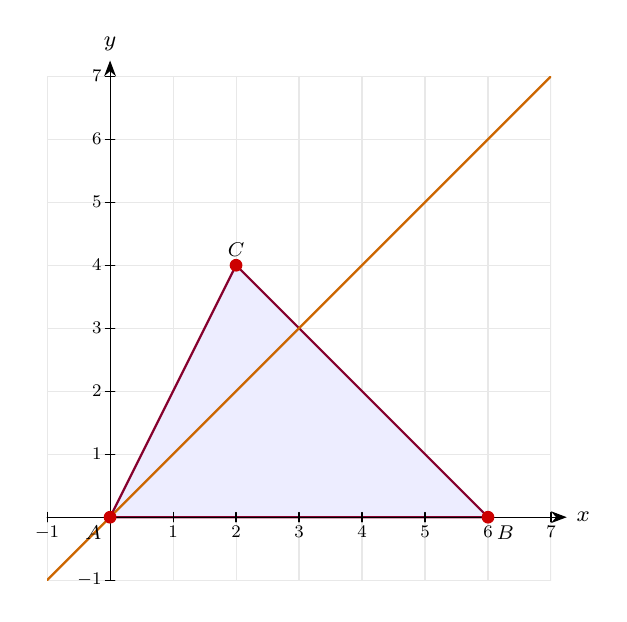
\begin{tikzpicture}[>={Stealth[length=2mm]},font=\footnotesize,line cap=round]
\begin{scope}
\clip (0,0) rectangle (6.4,6.4);
\draw[gray!18] (0,0) grid[xstep=0.8,ystep=0.8] (6.4,6.4);
\fill[blue!7] (0.8,0.8) -- (5.6,0.8) -- (2.4,4) -- cycle;
\draw[purple!70!black,thick] (0.8,0.8) -- (5.6,0.8) -- (2.4,4) -- cycle;
\draw[orange!80!black,thick] (0,0) -- (6.4,6.4);
\end{scope}
\draw[->] (0,0.8) -- (6.6,0.8) node[right]{$x$};
\draw[->] (0.8,0) -- (0.8,6.6) node[above]{$y$};
\draw (0,0.74) -- (0,0.86) node[below=2pt,scale=0.8]{$-1$};
\draw (1.6,0.74) -- (1.6,0.86) node[below=2pt,scale=0.8]{$1$};
\draw (2.4,0.74) -- (2.4,0.86) node[below=2pt,scale=0.8]{$2$};
\draw (3.2,0.74) -- (3.2,0.86) node[below=2pt,scale=0.8]{$3$};
\draw (4,0.74) -- (4,0.86) node[below=2pt,scale=0.8]{$4$};
\draw (4.8,0.74) -- (4.8,0.86) node[below=2pt,scale=0.8]{$5$};
\draw (5.6,0.74) -- (5.6,0.86) node[below=2pt,scale=0.8]{$6$};
\draw (6.4,0.74) -- (6.4,0.86) node[below=2pt,scale=0.8]{$7$};
\draw (0.74,0) -- (0.86,0) node[left=2pt,scale=0.8]{$-1$};
\draw (0.74,1.6) -- (0.86,1.6) node[left=2pt,scale=0.8]{$1$};
\draw (0.74,2.4) -- (0.86,2.4) node[left=2pt,scale=0.8]{$2$};
\draw (0.74,3.2) -- (0.86,3.2) node[left=2pt,scale=0.8]{$3$};
\draw (0.74,4) -- (0.86,4) node[left=2pt,scale=0.8]{$4$};
\draw (0.74,4.8) -- (0.86,4.8) node[left=2pt,scale=0.8]{$5$};
\draw (0.74,5.6) -- (0.86,5.6) node[left=2pt,scale=0.8]{$6$};
\draw (0.74,6.4) -- (0.86,6.4) node[left=2pt,scale=0.8]{$7$};
\fill[red!80!black] (0.8,0.8) circle (2.3pt);
\node[below left,scale=0.9] at (0.8,0.8) {$A$};
\fill[red!80!black] (5.6,0.8) circle (2.3pt);
\node[below right,scale=0.9] at (5.6,0.8) {$B$};
\fill[red!80!black] (2.4,4) circle (2.3pt);
\node[above,scale=0.9] at (2.4,4) {$C$};
\end{tikzpicture}
}
\end{center}
\small The line(s) and key points shown on the coordinate plane.\normalsize

\medskip\hrule

\section*{Parallel and Perpendicular Lines 52\quad\small\texttt{(cg3-052)}}
\addcontentsline{toc}{section}{Parallel and Perpendicular Lines 52 (cg3-052)}
\textit{Difficulty: Foundation \quad\textbar\quad Marks: 2}

\question{Find the perpendicular distance from \( (2, -1) \) to the line \( 4x + 3y - 7 = 0 \).}

\textbf{Worked solution.}

\textit{Distance formula}
\[\begin{gathered}
d = \frac{|4(2) + 3(-1) - 7|}{\sqrt{16+9}} = \frac{|8-3-7|}{5} = \frac{2}{5}
\end{gathered}\]
The perpendicular distance from \( (x_0, y_0) \) to \( ax + by + c = 0 \) is \( \frac{|ax_0 + by_0 + c|}{\sqrt{a^2 + b^2}} \). The absolute value handles either side of the line.

\begin{answerbox}
\textbf{Final answer:}\quad \(\displaystyle \frac{2}{5}\)
\end{answerbox}
\textbf{Diagram.}

\begin{center}
\resizebox{\ifdim\width>\linewidth \linewidth\else \width\fi}{!}{%
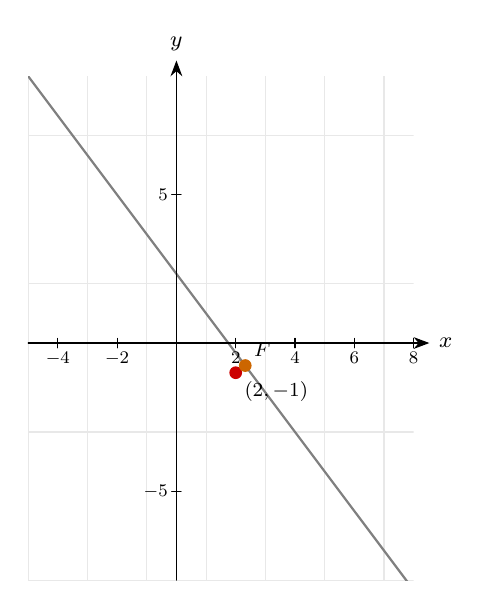
\begin{tikzpicture}[>={Stealth[length=2mm]},font=\footnotesize,line cap=round]
\begin{scope}
\clip (0,0) rectangle (4.894,6.4);
\draw[gray!18] (-0.376,-0.753) grid[xstep=0.753,ystep=1.882] (4.894,6.4);
\draw[gray,thick] (0,6.4) -- (4.894,-0.125);
\draw[dashed,orange!80!black,very thick] (2.635,2.635) -- (2.756,2.726);
\end{scope}
\draw[->] (0,3.012) -- (5.094,3.012) node[right]{$x$};
\draw[->] (1.882,0) -- (1.882,6.6) node[above]{$y$};
\draw (0.376,2.952) -- (0.376,3.072) node[below=2pt,scale=0.8]{$-4$};
\draw (1.129,2.952) -- (1.129,3.072) node[below=2pt,scale=0.8]{$-2$};
\draw (2.635,2.952) -- (2.635,3.072) node[below=2pt,scale=0.8]{$2$};
\draw (3.388,2.952) -- (3.388,3.072) node[below=2pt,scale=0.8]{$4$};
\draw (4.141,2.952) -- (4.141,3.072) node[below=2pt,scale=0.8]{$6$};
\draw (4.894,2.952) -- (4.894,3.072) node[below=2pt,scale=0.8]{$8$};
\draw (1.822,1.129) -- (1.942,1.129) node[left=2pt,scale=0.8]{$-5$};
\draw (1.822,4.894) -- (1.942,4.894) node[left=2pt,scale=0.8]{$5$};
\fill[red!80!black] (2.635,2.635) circle (2.3pt);
\node[below right,scale=0.9] at (2.635,2.635) {$(2,-1)$};
\fill[orange!80!black] (2.756,2.726) circle (2.3pt);
\node[above right,scale=0.9] at (2.756,2.726) {$F$};
\end{tikzpicture}
}
\end{center}
\small The line(s) and key points shown on the coordinate plane.\normalsize

\medskip\hrule

\section*{Parallel and Perpendicular Lines 53\quad\small\texttt{(cg3-053)}}
\addcontentsline{toc}{section}{Parallel and Perpendicular Lines 53 (cg3-053)}
\textit{Difficulty: Foundation \quad\textbar\quad Marks: 3}

\question{The lines \( y = 2x + c \) and \( y = 2x + d \) are 3 units apart. Find \( |c - d| \).}

\textbf{Worked solution.}

\textit{Step 1: Distance between parallel lines}
\[\begin{gathered}
d = \frac{|c - d|}{\sqrt{1 + 4}} = \frac{|c-d|}{\sqrt{5}}
\end{gathered}\]
Rewrite as 2x - y + c = 0 and 2x - y + d = 0.

\textit{Step 2: Solve}
\[\begin{gathered}
\frac{|c-d|}{\sqrt{5}} = 3 \implies |c - d| = 3\sqrt{5}
\end{gathered}\]
Multiply both sides by \( \sqrt{5} \) to isolate \( |c - d| \).

\begin{answerbox}
\textbf{Final answer:}\quad \(\displaystyle |c - d| = 3\sqrt{5}\)
\end{answerbox}
\textbf{Diagram.}

\begin{center}
\resizebox{\ifdim\width>\linewidth \linewidth\else \width\fi}{!}{%
\begin{tikzpicture}[>={Stealth[length=2mm]},font=\footnotesize,line cap=round]
\begin{scope}
\clip (0,0) rectangle (2.56,6.4);
\draw[gray!18] (-0.256,-0.256) grid[xstep=0.512,ystep=1.28] (2.56,6.4);
\draw[blue!70!black,thick] (0,-0.256) -- (2.56,4.864);
\draw[teal!70!black,thick] (0,1.459) -- (2.56,6.579);
\end{scope}
\draw[->] (0,2.304) -- (2.76,2.304) node[right]{$x$};
\draw[->] (1.28,0) -- (1.28,6.6) node[above]{$y$};
\draw (0.256,2.244) -- (0.256,2.364) node[below=2pt,scale=0.8]{$-4$};
\draw (0.768,2.244) -- (0.768,2.364) node[below=2pt,scale=0.8]{$-2$};
\draw (1.792,2.244) -- (1.792,2.364) node[below=2pt,scale=0.8]{$2$};
\draw (2.304,2.244) -- (2.304,2.364) node[below=2pt,scale=0.8]{$4$};
\draw (1.22,1.024) -- (1.34,1.024) node[left=2pt,scale=0.8]{$-5$};
\draw (1.22,3.584) -- (1.34,3.584) node[left=2pt,scale=0.8]{$5$};
\draw (1.22,4.864) -- (1.34,4.864) node[left=2pt,scale=0.8]{$10$};
\draw (1.22,6.144) -- (1.34,6.144) node[left=2pt,scale=0.8]{$15$};
\end{tikzpicture}
}
\end{center}
\small The line(s) and key points shown on the coordinate plane.\normalsize

\medskip\hrule

\section*{Parallel and Perpendicular Lines 54\quad\small\texttt{(cg3-054)}}
\addcontentsline{toc}{section}{Parallel and Perpendicular Lines 54 (cg3-054)}
\textit{Difficulty: Foundation \quad\textbar\quad Marks: 3}

\question{Find the equation of the line through \( (5, -3) \) parallel to \( 2x + 7y = 14 \). Give your answer in the form \( ax + by + c = 0 \).}

\textbf{Worked solution.}

\textit{Step 1: Gradient}
\[\begin{gathered}
m = -\frac{2}{7}
\end{gathered}\]
From \( 2x + 7y = 14 \): \( 7y = -2x + 14 \), so the gradient is \( -\tfrac{2}{7} \). Parallel lines share this.

\textit{Step 2: Equation}
\[\begin{gathered}
y + 3 = -\frac{2}{7}(x - 5) \implies 7y + 21 = -2x + 10 \implies 2x + 7y + 11 = 0
\end{gathered}\]
Use point-slope through \( (5, -3) \), multiply by \( 7 \) to clear the fraction, then collect everything on one side.

\begin{answerbox}
\textbf{Final answer:}\quad \(\displaystyle 2x + 7y + 11 = 0\)
\end{answerbox}
\textbf{Diagram.}

\begin{center}
\resizebox{\ifdim\width>\linewidth \linewidth\else \width\fi}{!}{%
\begin{tikzpicture}[>={Stealth[length=2mm]},font=\footnotesize,line cap=round]
\begin{scope}
\clip (0,0) rectangle (6.4,6.4);
\draw[gray!18] (0,0) grid[xstep=0.914,ystep=0.914] (6.4,6.4);
\draw[gray,thick] (0,5.747) -- (6.4,3.918);
\draw[blue!70!black,thick] (0,2.482) -- (6.4,0.653);
\end{scope}
\draw[->] (0,3.657) -- (6.6,3.657) node[right]{$x$};
\draw[->] (0.914,0) -- (0.914,6.6) node[above]{$y$};
\draw (0,3.597) -- (0,3.717) node[below=2pt,scale=0.8]{$-1$};
\draw (1.829,3.597) -- (1.829,3.717) node[below=2pt,scale=0.8]{$1$};
\draw (2.743,3.597) -- (2.743,3.717) node[below=2pt,scale=0.8]{$2$};
\draw (3.657,3.597) -- (3.657,3.717) node[below=2pt,scale=0.8]{$3$};
\draw (4.571,3.597) -- (4.571,3.717) node[below=2pt,scale=0.8]{$4$};
\draw (5.486,3.597) -- (5.486,3.717) node[below=2pt,scale=0.8]{$5$};
\draw (6.4,3.597) -- (6.4,3.717) node[below=2pt,scale=0.8]{$6$};
\draw (0.854,0) -- (0.974,0) node[left=2pt,scale=0.8]{$-4$};
\draw (0.854,0.914) -- (0.974,0.914) node[left=2pt,scale=0.8]{$-3$};
\draw (0.854,1.829) -- (0.974,1.829) node[left=2pt,scale=0.8]{$-2$};
\draw (0.854,2.743) -- (0.974,2.743) node[left=2pt,scale=0.8]{$-1$};
\draw (0.854,4.571) -- (0.974,4.571) node[left=2pt,scale=0.8]{$1$};
\draw (0.854,5.486) -- (0.974,5.486) node[left=2pt,scale=0.8]{$2$};
\draw (0.854,6.4) -- (0.974,6.4) node[left=2pt,scale=0.8]{$3$};
\fill[red!80!black] (5.486,0.914) circle (2.3pt);
\node[below right,scale=0.9] at (5.486,0.914) {$(5,-3)$};
\end{tikzpicture}
}
\end{center}
\small The line(s) and key points shown on the coordinate plane.\normalsize

\medskip\hrule

\section*{Parallel and Perpendicular Lines 55\quad\small\texttt{(cg3-055)}}
\addcontentsline{toc}{section}{Parallel and Perpendicular Lines 55 (cg3-055)}
\textit{Difficulty: Foundation \quad\textbar\quad Marks: 3}

\question{Two perpendicular lines meet at \( (3, 4) \). One has gradient 2. Find the equations of both lines.}

\textbf{Worked solution.}

\textit{Step 1: Line 1}
\[\begin{gathered}
y - 4 = 2(x - 3) \implies y = 2x - 2
\end{gathered}\]
Use point-slope through \( (3, 4) \) with gradient \( 2 \), then expand: \( 2(x-3) = 2x - 6 \), then add \( 4 \).

\textit{Step 2: Line 2 (perpendicular)}
\[\begin{gathered}
y - 4 = -\frac{1}{2}(x - 3) \implies y = -\frac{1}{2}x + \frac{11}{2}
\end{gathered}\]
Negative reciprocal of \( 2 \) is \( -\tfrac{1}{2} \). Expand and add: \( \tfrac{3}{2} + 4 = \tfrac{3}{2} + \tfrac{8}{2} = \tfrac{11}{2} \).

\begin{answerbox}
\textbf{Final answer:}\quad \(\displaystyle y = 2x - 2\) and \(\displaystyle y = -\frac{1}{2}x + \frac{11}{2}\)
\end{answerbox}
\textbf{Diagram.}

\begin{center}
\resizebox{\ifdim\width>\linewidth \linewidth\else \width\fi}{!}{%
\begin{tikzpicture}[>={Stealth[length=2mm]},font=\footnotesize,line cap=round]
\begin{scope}
\clip (0,0) rectangle (3.2,6.4);
\draw[gray!18] (0,-0.64) grid[xstep=0.64,ystep=1.28] (3.2,6.4);
\draw[blue!70!black,thick] (0,-0.64) -- (3.2,5.76);
\draw[teal!70!black,thick] (0,5.76) -- (3.2,4.16);
\end{scope}
\draw[->] (0,1.92) -- (3.4,1.92) node[right]{$x$};
\draw[->] (0.64,0) -- (0.64,6.6) node[above]{$y$};
\draw (0,1.86) -- (0,1.98) node[below=2pt,scale=0.8]{$-1$};
\draw (1.28,1.86) -- (1.28,1.98) node[below=2pt,scale=0.8]{$1$};
\draw (1.92,1.86) -- (1.92,1.98) node[below=2pt,scale=0.8]{$2$};
\draw (2.56,1.86) -- (2.56,1.98) node[below=2pt,scale=0.8]{$3$};
\draw (3.2,1.86) -- (3.2,1.98) node[below=2pt,scale=0.8]{$4$};
\draw (0.58,0.64) -- (0.7,0.64) node[left=2pt,scale=0.8]{$-2$};
\draw (0.58,3.2) -- (0.7,3.2) node[left=2pt,scale=0.8]{$2$};
\draw (0.58,4.48) -- (0.7,4.48) node[left=2pt,scale=0.8]{$4$};
\draw (0.58,5.76) -- (0.7,5.76) node[left=2pt,scale=0.8]{$6$};
\fill[red!80!black] (2.56,4.48) circle (2.3pt);
\node[above right,scale=0.9] at (2.56,4.48) {$(3,4)$};
\end{tikzpicture}
}
\end{center}
\small The line(s) and key points shown on the coordinate plane.\normalsize

\medskip\hrule

\section*{Parallel and Perpendicular Lines 56\quad\small\texttt{(cg3-056)}}
\addcontentsline{toc}{section}{Parallel and Perpendicular Lines 56 (cg3-056)}
\textit{Difficulty: Foundation \quad\textbar\quad Marks: 5}

\question{Show that the quadrilateral with vertices \( A(0,1) \), \( B(4,3) \), \( C(3,5) \), \( D(-1,3) \) is a rectangle.}

\textbf{Worked solution.}

\textit{Step 1: Gradient of AB}
\[\begin{gathered}
m_{AB} = \frac{2}{4} = \frac{1}{2}
\end{gathered}\]
\( m_{AB} = \tfrac{3 - 1}{4 - 0} = \tfrac{2}{4} = \tfrac{1}{2} \).

\textit{Step 2: Gradient of BC}
\[\begin{gathered}
m_{BC} = \frac{2}{-1} = -2
\end{gathered}\]
\( m_{BC} = \tfrac{5 - 3}{3 - 4} = \tfrac{2}{-1} = -2 \).

\textit{Step 3: Check perpendicular}
\[\begin{gathered}
\frac{1}{2} \times (-2) = -1 \checkmark
\end{gathered}\]
AB perp BC.

\textit{Step 4: Check parallel opposite sides}
\[\begin{gathered}
m_{CD} = \frac{-2}{-4} = \frac{1}{2} = m_{AB}; \quad m_{DA} = \frac{-2}{1} = -2 = m_{BC}
\end{gathered}\]
Opposite sides parallel and adjacent sides perpendicular: rectangle.

\begin{answerbox}
\textbf{Final answer:}\quad Opposite sides parallel, adjacent sides perpendicular: ABCD is a rectangle.
\end{answerbox}
\textbf{Diagram.}

\begin{center}
\resizebox{\ifdim\width>\linewidth \linewidth\else \width\fi}{!}{%
\begin{tikzpicture}[>={Stealth[length=2mm]},font=\footnotesize,line cap=round]
\begin{scope}
\clip (0,0) rectangle (6.4,6.4);
\draw[gray!18] (0,0) grid[xstep=0.914,ystep=0.914] (6.4,6.4);
\fill[blue!6] (1.829,1.829) -- (5.486,3.657) -- (4.571,5.486) -- (0.914,3.657) -- cycle;
\draw[purple!70!black,thick] (1.829,1.829) -- (5.486,3.657) -- (4.571,5.486) -- (0.914,3.657) -- cycle;
\end{scope}
\draw[->] (0,0.914) -- (6.6,0.914) node[right]{$x$};
\draw[->] (1.829,0) -- (1.829,6.6) node[above]{$y$};
\draw (0,0.854) -- (0,0.974) node[below=2pt,scale=0.8]{$-2$};
\draw (0.914,0.854) -- (0.914,0.974) node[below=2pt,scale=0.8]{$-1$};
\draw (2.743,0.854) -- (2.743,0.974) node[below=2pt,scale=0.8]{$1$};
\draw (3.657,0.854) -- (3.657,0.974) node[below=2pt,scale=0.8]{$2$};
\draw (4.571,0.854) -- (4.571,0.974) node[below=2pt,scale=0.8]{$3$};
\draw (5.486,0.854) -- (5.486,0.974) node[below=2pt,scale=0.8]{$4$};
\draw (6.4,0.854) -- (6.4,0.974) node[below=2pt,scale=0.8]{$5$};
\draw (1.769,0) -- (1.889,0) node[left=2pt,scale=0.8]{$-1$};
\draw (1.769,1.829) -- (1.889,1.829) node[left=2pt,scale=0.8]{$1$};
\draw (1.769,2.743) -- (1.889,2.743) node[left=2pt,scale=0.8]{$2$};
\draw (1.769,3.657) -- (1.889,3.657) node[left=2pt,scale=0.8]{$3$};
\draw (1.769,4.571) -- (1.889,4.571) node[left=2pt,scale=0.8]{$4$};
\draw (1.769,5.486) -- (1.889,5.486) node[left=2pt,scale=0.8]{$5$};
\draw (1.769,6.4) -- (1.889,6.4) node[left=2pt,scale=0.8]{$6$};
\fill[red!80!black] (1.829,1.829) circle (2.3pt);
\node[below,scale=0.9] at (1.829,1.829) {$A$};
\fill[red!80!black] (5.486,3.657) circle (2.3pt);
\node[right,scale=0.9] at (5.486,3.657) {$B$};
\fill[red!80!black] (4.571,5.486) circle (2.3pt);
\node[above,scale=0.9] at (4.571,5.486) {$C$};
\fill[red!80!black] (0.914,3.657) circle (2.3pt);
\node[left,scale=0.9] at (0.914,3.657) {$D$};
\end{tikzpicture}
}
\end{center}
\small The line(s) and key points shown on the coordinate plane.\normalsize

\medskip\hrule

\section*{Parallel and Perpendicular Lines 57\quad\small\texttt{(cg3-057)}}
\addcontentsline{toc}{section}{Parallel and Perpendicular Lines 57 (cg3-057)}
\textit{Difficulty: Foundation \quad\textbar\quad Marks: 3}

\question{The line \( L \) passes through \( (0, 5) \) perpendicular to \( y = -\frac{2}{3}x + 4 \). Where does \( L \) cross the x-axis?}

\textbf{Worked solution.}

\textit{Step 1: L has gradient 3/2}
\[\begin{gathered}
y = \frac{3}{2}x + 5
\end{gathered}\]
Negative reciprocal of \( -\tfrac{2}{3} \) is \( \tfrac{3}{2} \). Since the line passes through \( (0, 5) \), \( c = 5 \) directly.

\textit{Step 2: Set y = 0}
\[\begin{gathered}
0 = \frac{3}{2}x + 5 \implies x = -\frac{10}{3}
\end{gathered}\]
At the \( x \)-axis, \( y = 0 \). Solve \( \tfrac{3}{2}x = -5 \), giving \( x = -\tfrac{10}{3} \).

\begin{answerbox}
\textbf{Final answer:}\quad \(\displaystyle \left(-\frac{10}{3}, 0\right)\)
\end{answerbox}
\textbf{Diagram.}

\begin{center}
\resizebox{\ifdim\width>\linewidth \linewidth\else \width\fi}{!}{%
\begin{tikzpicture}[>={Stealth[length=2mm]},font=\footnotesize,line cap=round]
\begin{scope}
\clip (0,0) rectangle (4.267,6.4);
\draw[gray!18] (0,-0.711) grid[xstep=0.711,ystep=1.422] (4.267,6.4);
\draw[gray,thick] (0,5.926) -- (4.267,3.081);
\draw[blue!70!black,thick] (0,-1.067) -- (4.267,5.333);
\end{scope}
\draw[->] (0,0.711) -- (4.467,0.711) node[right]{$x$};
\draw[->] (3.556,0) -- (3.556,6.6) node[above]{$y$};
\draw (0,0.651) -- (0,0.771) node[below=2pt,scale=0.8]{$-5$};
\draw (0.711,0.651) -- (0.711,0.771) node[below=2pt,scale=0.8]{$-4$};
\draw (1.422,0.651) -- (1.422,0.771) node[below=2pt,scale=0.8]{$-3$};
\draw (2.133,0.651) -- (2.133,0.771) node[below=2pt,scale=0.8]{$-2$};
\draw (2.844,0.651) -- (2.844,0.771) node[below=2pt,scale=0.8]{$-1$};
\draw (4.267,0.651) -- (4.267,0.771) node[below=2pt,scale=0.8]{$1$};
\draw (3.496,2.133) -- (3.616,2.133) node[left=2pt,scale=0.8]{$2$};
\draw (3.496,3.556) -- (3.616,3.556) node[left=2pt,scale=0.8]{$4$};
\draw (3.496,4.978) -- (3.616,4.978) node[left=2pt,scale=0.8]{$6$};
\draw (3.496,6.4) -- (3.616,6.4) node[left=2pt,scale=0.8]{$8$};
\fill[red!80!black] (3.556,4.267) circle (2.3pt);
\node[left,scale=0.9] at (3.556,4.267) {$(0,5)$};
\fill[red!80!black] (1.185,0.711) circle (2.3pt);
\node[below left,scale=0.9] at (1.185,0.711) {$(-\tfrac{10}{3},0)$};
\end{tikzpicture}
}
\end{center}
\small The line(s) and key points shown on the coordinate plane.\normalsize

\medskip\hrule

\section*{Parallel and Perpendicular Lines 58\quad\small\texttt{(cg3-058)}}
\addcontentsline{toc}{section}{Parallel and Perpendicular Lines 58 (cg3-058)}
\textit{Difficulty: Foundation \quad\textbar\quad Marks: 4}

\question{Find the equation of the perpendicular bisector of the segment from \( (1, -3) \) to \( (5, 1) \).}

\textbf{Worked solution.}

\textit{Step 1: Midpoint}
\[\begin{gathered}
M = (3, -1)
\end{gathered}\]
Average coordinates: \( \tfrac{1+5}{2} = 3 \), \( \tfrac{-3+1}{2} = -1 \).

\textit{Step 2: Gradient of segment}
\[\begin{gathered}
m = \frac{4}{4} = 1
\end{gathered}\]
\( m = \tfrac{1 - (-3)}{5 - 1} = \tfrac{4}{4} = 1 \).

\textit{Step 3: Perpendicular bisector}
\[\begin{gathered}
m_{\perp} = -1; \quad y + 1 = -(x - 3) \implies y = -x + 2
\end{gathered}\]
Negative reciprocal of \( 1 \) is \( -1 \). Point-slope through the midpoint, then expand: \( -(x-3) = -x + 3 \), and subtract \( 1 \) from both sides.

\begin{answerbox}
\textbf{Final answer:}\quad \(\displaystyle y = -x + 2\)
\end{answerbox}
\textbf{Diagram.}

\begin{center}
\resizebox{\ifdim\width>\linewidth \linewidth\else \width\fi}{!}{%
\begin{tikzpicture}[>={Stealth[length=2mm]},font=\footnotesize,line cap=round]
\begin{scope}
\clip (0,0) rectangle (6.4,6.4);
\draw[gray!18] (0,0) grid[xstep=0.914,ystep=0.914] (6.4,6.4);
\draw[orange!80!black,thick] (0,6.4) -- (6.4,0);
\draw[gray,very thick] (1.829,0.914) -- (5.486,4.571);
\end{scope}
\draw[->] (0,3.657) -- (6.6,3.657) node[right]{$x$};
\draw[->] (0.914,0) -- (0.914,6.6) node[above]{$y$};
\draw (0,3.597) -- (0,3.717) node[below=2pt,scale=0.8]{$-1$};
\draw (1.829,3.597) -- (1.829,3.717) node[below=2pt,scale=0.8]{$1$};
\draw (2.743,3.597) -- (2.743,3.717) node[below=2pt,scale=0.8]{$2$};
\draw (3.657,3.597) -- (3.657,3.717) node[below=2pt,scale=0.8]{$3$};
\draw (4.571,3.597) -- (4.571,3.717) node[below=2pt,scale=0.8]{$4$};
\draw (5.486,3.597) -- (5.486,3.717) node[below=2pt,scale=0.8]{$5$};
\draw (6.4,3.597) -- (6.4,3.717) node[below=2pt,scale=0.8]{$6$};
\draw (0.854,0) -- (0.974,0) node[left=2pt,scale=0.8]{$-4$};
\draw (0.854,0.914) -- (0.974,0.914) node[left=2pt,scale=0.8]{$-3$};
\draw (0.854,1.829) -- (0.974,1.829) node[left=2pt,scale=0.8]{$-2$};
\draw (0.854,2.743) -- (0.974,2.743) node[left=2pt,scale=0.8]{$-1$};
\draw (0.854,4.571) -- (0.974,4.571) node[left=2pt,scale=0.8]{$1$};
\draw (0.854,5.486) -- (0.974,5.486) node[left=2pt,scale=0.8]{$2$};
\draw (0.854,6.4) -- (0.974,6.4) node[left=2pt,scale=0.8]{$3$};
\fill[red!80!black] (1.829,0.914) circle (2.3pt);
\fill[red!80!black] (5.486,4.571) circle (2.3pt);
\fill[orange!80!black] (3.657,2.743) circle (2.3pt);
\node[below right,scale=0.9] at (3.657,2.743) {$M$};
\end{tikzpicture}
}
\end{center}
\small The line(s) and key points shown on the coordinate plane.\normalsize

\medskip\hrule

\section*{Parallel and Perpendicular Lines 59\quad\small\texttt{(cg3-059)}}
\addcontentsline{toc}{section}{Parallel and Perpendicular Lines 59 (cg3-059)}
\textit{Difficulty: Foundation \quad\textbar\quad Marks: 2}

\question{The line \( y = mx + 3 \) is parallel to the line joining \( (1, 2) \) and \( (4, 8) \). Find \( m \).}

\textbf{Worked solution.}

\textit{Gradient of line through points}
\[\begin{gathered}
m = \frac{8-2}{4-1} = 2
\end{gathered}\]
Parallel means same gradient.

\begin{answerbox}
\textbf{Final answer:}\quad \(\displaystyle m = 2\)
\end{answerbox}
\textbf{Diagram.}

\begin{center}
\resizebox{\ifdim\width>\linewidth \linewidth\else \width\fi}{!}{%
\begin{tikzpicture}[>={Stealth[length=2mm]},font=\footnotesize,line cap=round]
\begin{scope}
\clip (0,0) rectangle (2.954,6.4);
\draw[gray!18] (0,-0.492) grid[xstep=0.492,ystep=0.985] (2.954,6.4);
\draw[gray,thick] (0,-0.492) -- (2.954,5.415);
\draw[blue!70!black,thick] (0,0.985) -- (2.954,6.892);
\end{scope}
\draw[->] (0,0.492) -- (3.154,0.492) node[right]{$x$};
\draw[->] (0.492,0) -- (0.492,6.6) node[above]{$y$};
\draw (0,0.432) -- (0,0.552) node[below=2pt,scale=0.8]{$-1$};
\draw (0.985,0.432) -- (0.985,0.552) node[below=2pt,scale=0.8]{$1$};
\draw (1.477,0.432) -- (1.477,0.552) node[below=2pt,scale=0.8]{$2$};
\draw (1.969,0.432) -- (1.969,0.552) node[below=2pt,scale=0.8]{$3$};
\draw (2.462,0.432) -- (2.462,0.552) node[below=2pt,scale=0.8]{$4$};
\draw (2.954,0.432) -- (2.954,0.552) node[below=2pt,scale=0.8]{$5$};
\draw (0.432,1.477) -- (0.552,1.477) node[left=2pt,scale=0.8]{$2$};
\draw (0.432,2.462) -- (0.552,2.462) node[left=2pt,scale=0.8]{$4$};
\draw (0.432,3.446) -- (0.552,3.446) node[left=2pt,scale=0.8]{$6$};
\draw (0.432,4.431) -- (0.552,4.431) node[left=2pt,scale=0.8]{$8$};
\draw (0.432,5.415) -- (0.552,5.415) node[left=2pt,scale=0.8]{$10$};
\draw (0.432,6.4) -- (0.552,6.4) node[left=2pt,scale=0.8]{$12$};
\fill[red!80!black] (0.985,1.477) circle (2.3pt);
\node[above right,scale=0.9] at (0.985,1.477) {$(1,2)$};
\fill[red!80!black] (2.462,4.431) circle (2.3pt);
\node[above right,scale=0.9] at (2.462,4.431) {$(4,8)$};
\end{tikzpicture}
}
\end{center}
\small The line(s) and key points shown on the coordinate plane.\normalsize

\medskip\hrule

\section*{Parallel and Perpendicular Lines 60\quad\small\texttt{(cg3-060)}}
\addcontentsline{toc}{section}{Parallel and Perpendicular Lines 60 (cg3-060)}
\textit{Difficulty: Foundation \quad\textbar\quad Marks: 3}

\question{Three lines have equations \( L_1: y = 3x \), \( L_2: y = -\frac{1}{3}x + 4 \), \( L_3: y = 3x - 5 \). Which pairs are parallel? Which are perpendicular?}

\textbf{Worked solution.}

\textit{Step 1: Compare gradients}
\[\begin{gathered}
m_1 = 3, m_2 = -\frac{1}{3}, m_3 = 3
\end{gathered}\]
Read each gradient straight from the \( y = mx + c \) form.

\textit{Step 2: Parallel}
\[\begin{gathered}
L_1 \parallel L_3 \text{ (both gradient 3)}
\end{gathered}\]
Equal gradients with different intercepts means the lines are parallel.

\textit{Step 3: Perpendicular}
\[\begin{gathered}
L_1 \perp L_2 \text{ and } L_2 \perp L_3 \text{ (product = -1)}
\end{gathered}\]
\( 3 \times (-\tfrac{1}{3}) = -1 \), so \( L_2 \) is perpendicular to both \( L_1 \) and \( L_3 \).

\begin{answerbox}
\textbf{Final answer:}\quad \(\displaystyle L_1\) parallel \(\displaystyle L_3\); \(\displaystyle L_1 \perp L_2\); \(\displaystyle L_2 \perp L_3\)
\end{answerbox}
\textbf{Diagram.}

\begin{center}
\resizebox{\ifdim\width>\linewidth \linewidth\else \width\fi}{!}{%
\begin{tikzpicture}[>={Stealth[length=2mm]},font=\footnotesize,line cap=round]
\begin{scope}
\clip (0,0) rectangle (2.065,6.4);
\draw[gray!18] (-0.206,-0.413) grid[xstep=0.413,ystep=1.032] (2.065,6.4);
\draw[blue!70!black,thick] (0,0.619) -- (2.065,6.813);
\draw[teal!70!black,thick] (0,4.886) -- (2.065,4.198);
\draw[gray,thick] (0,-0.413) -- (2.065,5.781);
\end{scope}
\draw[->] (0,3.716) -- (2.265,3.716) node[right]{$x$};
\draw[->] (1.032,0) -- (1.032,6.6) node[above]{$y$};
\draw (0.206,3.656) -- (0.206,3.776) node[below=2pt,scale=0.8]{$-4$};
\draw (0.619,3.656) -- (0.619,3.776) node[below=2pt,scale=0.8]{$-2$};
\draw (1.445,3.656) -- (1.445,3.776) node[below=2pt,scale=0.8]{$2$};
\draw (1.858,3.656) -- (1.858,3.776) node[below=2pt,scale=0.8]{$4$};
\draw (0.972,0.619) -- (1.092,0.619) node[left=2pt,scale=0.8]{$-15$};
\draw (0.972,1.652) -- (1.092,1.652) node[left=2pt,scale=0.8]{$-10$};
\draw (0.972,2.684) -- (1.092,2.684) node[left=2pt,scale=0.8]{$-5$};
\draw (0.972,4.748) -- (1.092,4.748) node[left=2pt,scale=0.8]{$5$};
\draw (0.972,5.781) -- (1.092,5.781) node[left=2pt,scale=0.8]{$10$};
\end{tikzpicture}
}
\end{center}
\small The line(s) and key points shown on the coordinate plane.\normalsize

\medskip\hrule

\section*{Parallel and Perpendicular Lines 61\quad\small\texttt{(cg3-061)}}
\addcontentsline{toc}{section}{Parallel and Perpendicular Lines 61 (cg3-061)}
\textit{Difficulty: Foundation \quad\textbar\quad Marks: 2}

\question{Find the reflection of the point \( (5, 2) \) in the line \( y = x \).}

\textbf{Worked solution.}

\textit{Reflection in y = x}
\[\begin{gathered}
(5, 2) \to (2, 5)
\end{gathered}\]
Swap coordinates.

\begin{answerbox}
\textbf{Final answer:}\quad \(\displaystyle (2, 5)\)
\end{answerbox}
\textbf{Diagram.}

\begin{center}
\resizebox{\ifdim\width>\linewidth \linewidth\else \width\fi}{!}{%
\begin{tikzpicture}[>={Stealth[length=2mm]},font=\footnotesize,line cap=round]
\begin{scope}
\clip (0,0) rectangle (6.4,6.4);
\draw[gray!18] (0,0) grid[xstep=0.914,ystep=0.914] (6.4,6.4);
\draw[gray,thick] (0,0) -- (6.4,6.4);
\end{scope}
\draw[->] (0,0.914) -- (6.6,0.914) node[right]{$x$};
\draw[->] (0.914,0) -- (0.914,6.6) node[above]{$y$};
\draw (0,0.854) -- (0,0.974) node[below=2pt,scale=0.8]{$-1$};
\draw (1.829,0.854) -- (1.829,0.974) node[below=2pt,scale=0.8]{$1$};
\draw (2.743,0.854) -- (2.743,0.974) node[below=2pt,scale=0.8]{$2$};
\draw (3.657,0.854) -- (3.657,0.974) node[below=2pt,scale=0.8]{$3$};
\draw (4.571,0.854) -- (4.571,0.974) node[below=2pt,scale=0.8]{$4$};
\draw (5.486,0.854) -- (5.486,0.974) node[below=2pt,scale=0.8]{$5$};
\draw (6.4,0.854) -- (6.4,0.974) node[below=2pt,scale=0.8]{$6$};
\draw (0.854,0) -- (0.974,0) node[left=2pt,scale=0.8]{$-1$};
\draw (0.854,1.829) -- (0.974,1.829) node[left=2pt,scale=0.8]{$1$};
\draw (0.854,2.743) -- (0.974,2.743) node[left=2pt,scale=0.8]{$2$};
\draw (0.854,3.657) -- (0.974,3.657) node[left=2pt,scale=0.8]{$3$};
\draw (0.854,4.571) -- (0.974,4.571) node[left=2pt,scale=0.8]{$4$};
\draw (0.854,5.486) -- (0.974,5.486) node[left=2pt,scale=0.8]{$5$};
\draw (0.854,6.4) -- (0.974,6.4) node[left=2pt,scale=0.8]{$6$};
\fill[red!80!black] (5.486,2.743) circle (2.3pt);
\node[below right,scale=0.9] at (5.486,2.743) {$(5,2)$};
\fill[red!80!black] (2.743,5.486) circle (2.3pt);
\node[above left,scale=0.9] at (2.743,5.486) {$(2,5)$};
\end{tikzpicture}
}
\end{center}
\small The line(s) and key points shown on the coordinate plane.\normalsize

\medskip\hrule

\section*{Parallel and Perpendicular Lines 62\quad\small\texttt{(cg3-062)}}
\addcontentsline{toc}{section}{Parallel and Perpendicular Lines 62 (cg3-062)}
\textit{Difficulty: Foundation \quad\textbar\quad Marks: 3}

\question{Find the value of \( a \) if the line \( ax + 6y = 12 \) is perpendicular to \( 2x + 3y = 9 \).}

\textbf{Worked solution.}

\textit{Step 1: Gradients}
\[\begin{gathered}
m_1 = -\frac{a}{6}; \quad m_2 = -\frac{2}{3}
\end{gathered}\]
Rearrange each line into \( y = mx + c \) form to read off the gradients.

\textit{Step 2: Product = -1}
\[\begin{gathered}
\left(-\frac{a}{6}\right) \times \left(-\frac{2}{3}\right) = -1 \implies \frac{a}{9} = -1 \implies a = -9
\end{gathered}\]
Two non-vertical lines are perpendicular if and only if their gradients multiply to \( -1 \). Be careful with the double negative --- \( (-)(-)=+ \) so the product is \( +\tfrac{a}{9} \).

\begin{answerbox}
\textbf{Final answer:}\quad \(\displaystyle a = -9\)
\end{answerbox}
\textbf{Diagram.}

\begin{center}
\resizebox{\ifdim\width>\linewidth \linewidth\else \width\fi}{!}{%
\begin{tikzpicture}[>={Stealth[length=2mm]},font=\footnotesize,line cap=round]
\begin{scope}
\clip (0,0) rectangle (4.571,6.4);
\draw[gray!18] (-0.457,-0.457) grid[xstep=0.914,ystep=0.914] (4.571,6.4);
\draw[gray,thick] (0,5.181) -- (4.571,2.133);
\draw[blue!70!black,thick] (0,-0.229) -- (4.571,6.629);
\end{scope}
\draw[->] (0,2.286) -- (4.771,2.286) node[right]{$x$};
\draw[->] (2.286,0) -- (2.286,6.6) node[above]{$y$};
\draw (0.457,2.226) -- (0.457,2.346) node[below=2pt,scale=0.8]{$-4$};
\draw (1.371,2.226) -- (1.371,2.346) node[below=2pt,scale=0.8]{$-2$};
\draw (3.2,2.226) -- (3.2,2.346) node[below=2pt,scale=0.8]{$2$};
\draw (4.114,2.226) -- (4.114,2.346) node[below=2pt,scale=0.8]{$4$};
\draw (2.226,0.457) -- (2.346,0.457) node[left=2pt,scale=0.8]{$-4$};
\draw (2.226,1.371) -- (2.346,1.371) node[left=2pt,scale=0.8]{$-2$};
\draw (2.226,3.2) -- (2.346,3.2) node[left=2pt,scale=0.8]{$2$};
\draw (2.226,4.114) -- (2.346,4.114) node[left=2pt,scale=0.8]{$4$};
\draw (2.226,5.029) -- (2.346,5.029) node[left=2pt,scale=0.8]{$6$};
\draw (2.226,5.943) -- (2.346,5.943) node[left=2pt,scale=0.8]{$8$};
\end{tikzpicture}
}
\end{center}
\small The line(s) and key points shown on the coordinate plane.\normalsize

\medskip\hrule

\section*{Parallel and Perpendicular Lines 63\quad\small\texttt{(cg3-063)}}
\addcontentsline{toc}{section}{Parallel and Perpendicular Lines 63 (cg3-063)}
\textit{Difficulty: Foundation \quad\textbar\quad Marks: 3}

\question{A rhombus has vertices at \( (0, 3) \), \( (4, 0) \), \( (0, -3) \), \( (-4, 0) \). Show that its diagonals are perpendicular.}

\textbf{Worked solution.}

\textit{Diagonal gradients}
\[\begin{gathered}
m_1 = \frac{3-(-3)}{0-0} = \text{undefined (vertical)}; \quad m_2 = \frac{0-0}{4-(-4)} = 0 \text{ (horizontal)}
\end{gathered}\]
Vertical and horizontal lines are perpendicular.

\begin{answerbox}
\textbf{Final answer:}\quad One diagonal is vertical, the other horizontal: they are perpendicular.
\end{answerbox}
\textbf{Diagram.}

\begin{center}
\resizebox{\ifdim\width>\linewidth \linewidth\else \width\fi}{!}{%
\begin{tikzpicture}[>={Stealth[length=2mm]},font=\footnotesize,line cap=round]
\begin{scope}
\clip (0,0) rectangle (8,6.4);
\draw[gray!18] (-0.8,0) grid[xstep=1.6,ystep=0.8] (8,6.4);
\fill[blue!6] (4,5.6) -- (7.2,3.2) -- (4,0.8) -- (0.8,3.2) -- cycle;
\draw[purple!70!black,thick] (4,5.6) -- (7.2,3.2) -- (4,0.8) -- (0.8,3.2) -- cycle;
\draw[dashed,purple!70!black,very thick] (4,5.6) -- (4,0.8);
\draw[dashed,purple!70!black,very thick] (0.8,3.2) -- (7.2,3.2);
\end{scope}
\draw[->] (0,3.2) -- (8.2,3.2) node[right]{$x$};
\draw[->] (4,0) -- (4,6.6) node[above]{$y$};
\draw (0.8,3.14) -- (0.8,3.26) node[below=2pt,scale=0.8]{$-4$};
\draw (2.4,3.14) -- (2.4,3.26) node[below=2pt,scale=0.8]{$-2$};
\draw (5.6,3.14) -- (5.6,3.26) node[below=2pt,scale=0.8]{$2$};
\draw (7.2,3.14) -- (7.2,3.26) node[below=2pt,scale=0.8]{$4$};
\draw (3.94,0) -- (4.06,0) node[left=2pt,scale=0.8]{$-4$};
\draw (3.94,0.8) -- (4.06,0.8) node[left=2pt,scale=0.8]{$-3$};
\draw (3.94,1.6) -- (4.06,1.6) node[left=2pt,scale=0.8]{$-2$};
\draw (3.94,2.4) -- (4.06,2.4) node[left=2pt,scale=0.8]{$-1$};
\draw (3.94,4) -- (4.06,4) node[left=2pt,scale=0.8]{$1$};
\draw (3.94,4.8) -- (4.06,4.8) node[left=2pt,scale=0.8]{$2$};
\draw (3.94,5.6) -- (4.06,5.6) node[left=2pt,scale=0.8]{$3$};
\draw (3.94,6.4) -- (4.06,6.4) node[left=2pt,scale=0.8]{$4$};
\end{tikzpicture}
}
\end{center}
\small The line(s) and key points shown on the coordinate plane.\normalsize

\medskip\hrule

\section*{Parallel and Perpendicular Lines 64\quad\small\texttt{(cg3-064)}}
\addcontentsline{toc}{section}{Parallel and Perpendicular Lines 64 (cg3-064)}
\textit{Difficulty: Foundation \quad\textbar\quad Marks: 5}

\question{Find the area of the triangle formed by \( y = 2x \), \( y = -\frac{1}{2}x + 5 \), and the x-axis.}

\textbf{Worked solution.}

\textit{Step 1: Intersection of the two lines}
\[\begin{gathered}
2x = -\frac{1}{2}x + 5 \implies \frac{5}{2}x = 5 \implies x = 2, y = 4
\end{gathered}\]
Equate the two \( y \)-expressions to find where the lines meet. This is the apex of the triangle.

\textit{Step 2: x-intercepts}
\[\begin{gathered}
y = 2x: x = 0; \quad y = -\frac{1}{2}x + 5: x = 10
\end{gathered}\]
Set \( y = 0 \) in each line. \( y = 2x \) passes through the origin; \( y = -\tfrac{1}{2}x + 5 \) crosses the \( x \)-axis at \( x = 10 \). These give the base of the triangle on the \( x \)-axis.

\textit{Step 3: Area}
\[\begin{gathered}
\text{Area} = \frac{1}{2} \times 10 \times 4 = 20
\end{gathered}\]
Base along x-axis = 10, height = 4.

\begin{answerbox}
\textbf{Final answer:}\quad \(\displaystyle 20\) square units
\end{answerbox}
\textbf{Diagram.}

\begin{center}
\resizebox{\ifdim\width>\linewidth \linewidth\else \width\fi}{!}{%
\begin{tikzpicture}[>={Stealth[length=2mm]},font=\footnotesize,line cap=round]
\begin{scope}
\clip (0,0) rectangle (3.491,6.4);
\draw[gray!18] (-0.291,-1.164) grid[xstep=0.582,ystep=1.455] (3.491,6.4);
\fill[blue!7] (0.291,0.291) -- (3.2,0.291) -- (0.873,1.455) -- cycle;
\draw[purple!70!black,thick] (0.291,0.291) -- (3.2,0.291) -- (0.873,1.455) -- cycle;
\draw[blue!70!black,thick] (0,-0.291) -- (3.491,6.691);
\draw[teal!70!black,thick] (0,1.891) -- (3.491,0.145);
\end{scope}
\draw[->] (0,0.291) -- (3.691,0.291) node[right]{$x$};
\draw[->] (0.291,0) -- (0.291,6.6) node[above]{$y$};
\draw (0.873,0.231) -- (0.873,0.351) node[below=2pt,scale=0.8]{$2$};
\draw (1.455,0.231) -- (1.455,0.351) node[below=2pt,scale=0.8]{$4$};
\draw (2.036,0.231) -- (2.036,0.351) node[below=2pt,scale=0.8]{$6$};
\draw (2.618,0.231) -- (2.618,0.351) node[below=2pt,scale=0.8]{$8$};
\draw (3.2,0.231) -- (3.2,0.351) node[below=2pt,scale=0.8]{$10$};
\draw (0.231,1.745) -- (0.351,1.745) node[left=2pt,scale=0.8]{$5$};
\draw (0.231,3.2) -- (0.351,3.2) node[left=2pt,scale=0.8]{$10$};
\draw (0.231,4.655) -- (0.351,4.655) node[left=2pt,scale=0.8]{$15$};
\draw (0.231,6.109) -- (0.351,6.109) node[left=2pt,scale=0.8]{$20$};
\fill[red!80!black] (0.291,0.291) circle (2.3pt);
\node[below left,scale=0.9] at (0.291,0.291) {$O$};
\fill[red!80!black] (3.2,0.291) circle (2.3pt);
\fill[red!80!black] (0.873,1.455) circle (2.3pt);
\end{tikzpicture}
}
\end{center}
\small The line(s) and key points shown on the coordinate plane.\normalsize

\medskip\hrule

\section*{Parallel and Perpendicular Lines 65\quad\small\texttt{(cg3-065)}}
\addcontentsline{toc}{section}{Parallel and Perpendicular Lines 65 (cg3-065)}
\textit{Difficulty: Foundation \quad\textbar\quad Marks: 5}

\question{The perpendicular from \( A(0, 4) \) to \( y = 2x - 3 \) meets the line at \( B \). Find the coordinates of \( B \) and the length \( AB \).}

\textbf{Worked solution.}

\textit{Step 1: Perpendicular from A}
\[\begin{gathered}
y - 4 = -\frac{1}{2}(x - 0) \implies y = -\frac{1}{2}x + 4
\end{gathered}\]
Negative reciprocal of \( 2 \) is \( -\tfrac{1}{2} \). Point-slope through \( A(0, 4) \); since \( x_1 = 0 \) the \( y \)-intercept is \( 4 \) directly.

\textit{Step 2: Solve with y = 2x - 3}
\[\begin{gathered}
2x - 3 = -\frac{1}{2}x + 4 \implies \frac{5}{2}x = 7 \implies x = \frac{14}{5}, y = \frac{13}{5}
\end{gathered}\]
Equate the two lines. Collect \( x \)-terms: \( 2x + \tfrac{1}{2}x = \tfrac{5}{2}x \); the constants give \( 7 \). Multiply by \( \tfrac{2}{5} \) to find \( x \), then back-substitute.

\textit{Step 3: Distance}
\[\begin{gathered}
AB = \sqrt{\frac{196}{25} + \frac{49}{25}} = \sqrt{\frac{245}{25}} = \frac{7\sqrt{5}}{5}
\end{gathered}\]
Apply the distance formula: \( \left(\tfrac{14}{5}\right)^2 = \tfrac{196}{25} \) and \( \left(\tfrac{13}{5} - 4\right)^2 = \left(-\tfrac{7}{5}\right)^2 = \tfrac{49}{25} \). Then \( \sqrt{245} = \sqrt{49 \times 5} = 7\sqrt{5} \).

\begin{answerbox}
\textbf{Final answer:}\quad \(\displaystyle B = \left(\frac{14}{5}, \frac{13}{5}\right)\); \(\displaystyle AB = \frac{7\sqrt{5}}{5}\)
\end{answerbox}
\textbf{Diagram.}

\begin{center}
\resizebox{\ifdim\width>\linewidth \linewidth\else \width\fi}{!}{%
\begin{tikzpicture}[>={Stealth[length=2mm]},font=\footnotesize,line cap=round]
\begin{scope}
\clip (0,0) rectangle (3.467,6.4);
\draw[gray!18] (-0.267,-0.8) grid[xstep=0.533,ystep=1.333] (3.467,6.4);
\draw[gray,thick] (0,-0.267) -- (3.467,6.667);
\draw[dashed,orange!80!black,very thick] (1.333,4.267) -- (2.08,3.893);
\end{scope}
\draw[->] (0,3.2) -- (3.667,3.2) node[right]{$x$};
\draw[->] (1.333,0) -- (1.333,6.6) node[above]{$y$};
\draw (0.267,3.14) -- (0.267,3.26) node[below=2pt,scale=0.8]{$-4$};
\draw (0.8,3.14) -- (0.8,3.26) node[below=2pt,scale=0.8]{$-2$};
\draw (1.867,3.14) -- (1.867,3.26) node[below=2pt,scale=0.8]{$2$};
\draw (2.4,3.14) -- (2.4,3.26) node[below=2pt,scale=0.8]{$4$};
\draw (2.933,3.14) -- (2.933,3.26) node[below=2pt,scale=0.8]{$6$};
\draw (3.467,3.14) -- (3.467,3.26) node[below=2pt,scale=0.8]{$8$};
\draw (1.273,0.533) -- (1.393,0.533) node[left=2pt,scale=0.8]{$-10$};
\draw (1.273,1.867) -- (1.393,1.867) node[left=2pt,scale=0.8]{$-5$};
\draw (1.273,4.533) -- (1.393,4.533) node[left=2pt,scale=0.8]{$5$};
\draw (1.273,5.867) -- (1.393,5.867) node[left=2pt,scale=0.8]{$10$};
\fill[red!80!black] (1.333,4.267) circle (2.3pt);
\node[above left,scale=0.9] at (1.333,4.267) {$A$};
\fill[orange!80!black] (2.08,3.893) circle (2.3pt);
\node[below right,scale=0.9] at (2.08,3.893) {$B$};
\end{tikzpicture}
}
\end{center}
\small The line(s) and key points shown on the coordinate plane.\normalsize

\medskip\hrule

\section*{Parallel and Perpendicular Lines 66\quad\small\texttt{(cg3-066)}}
\addcontentsline{toc}{section}{Parallel and Perpendicular Lines 66 (cg3-066)}
\textit{Difficulty: Foundation \quad\textbar\quad Marks: 3}

\question{The line \( L_1 \) has equation \( 5x - y = 10 \). The line \( L_2 \) is parallel to \( L_1 \) and passes through \( (-1, 3) \). Find where \( L_2 \) crosses the y-axis.}

\textbf{Worked solution.}

\textit{Step 1: Gradient}
\[\begin{gathered}
m = 5
\end{gathered}\]
From \( 5x - y = 10 \): \( y = 5x - 10 \), so the gradient is \( 5 \). Parallel lines share gradients.

\textit{Step 2: L2 equation}
\[\begin{gathered}
y - 3 = 5(x + 1) \implies y = 5x + 8
\end{gathered}\]
Point-slope through \( (-1, 3) \). Expand: \( 5(x+1) = 5x + 5 \), then add \( 3 \). y-intercept is \( 8 \).

\begin{answerbox}
\textbf{Final answer:}\quad \(\displaystyle (0, 8)\)
\end{answerbox}
\textbf{Diagram.}

\begin{center}
\resizebox{\ifdim\width>\linewidth \linewidth\else \width\fi}{!}{%
\begin{tikzpicture}[>={Stealth[length=2mm]},font=\footnotesize,line cap=round]
\begin{scope}
\clip (0,0) rectangle (1.083,6.4);
\draw[gray!18] (0,-0.394) grid[xstep=0.197,ystep=0.985] (1.083,6.4);
\draw[gray,thick] (0,-0.394) -- (1.083,5.022);
\draw[blue!70!black,thick] (0,1.378) -- (1.083,6.794);
\end{scope}
\draw[->] (0,3.545) -- (1.283,3.545) node[right]{$x$};
\draw[->] (0.591,0) -- (0.591,6.6) node[above]{$y$};
\draw (0,3.485) -- (0,3.605) node[below=2pt,scale=0.8]{$-6$};
\draw (0.197,3.485) -- (0.197,3.605) node[below=2pt,scale=0.8]{$-4$};
\draw (0.394,3.485) -- (0.394,3.605) node[below=2pt,scale=0.8]{$-2$};
\draw (0.788,3.485) -- (0.788,3.605) node[below=2pt,scale=0.8]{$2$};
\draw (0.985,3.485) -- (0.985,3.605) node[below=2pt,scale=0.8]{$4$};
\draw (0.531,0.591) -- (0.651,0.591) node[left=2pt,scale=0.8]{$-30$};
\draw (0.531,1.575) -- (0.651,1.575) node[left=2pt,scale=0.8]{$-20$};
\draw (0.531,2.56) -- (0.651,2.56) node[left=2pt,scale=0.8]{$-10$};
\draw (0.531,4.529) -- (0.651,4.529) node[left=2pt,scale=0.8]{$10$};
\draw (0.531,5.514) -- (0.651,5.514) node[left=2pt,scale=0.8]{$20$};
\fill[red!80!black] (0.492,3.84) circle (2.3pt);
\node[left,scale=0.9] at (0.492,3.84) {$(-1,3)$};
\fill[red!80!black] (0.591,4.332) circle (2.3pt);
\node[left,scale=0.9] at (0.591,4.332) {$(0,8)$};
\end{tikzpicture}
}
\end{center}
\small The line(s) and key points shown on the coordinate plane.\normalsize

\medskip\hrule

\section*{Parallel and Perpendicular Lines 67\quad\small\texttt{(cg3-067)}}
\addcontentsline{toc}{section}{Parallel and Perpendicular Lines 67 (cg3-067)}
\textit{Difficulty: Foundation \quad\textbar\quad Marks: 5}

\question{Two lines are \( L_1: y = ax + 3 \) and \( L_2: y = (2a+1)x - 5 \). Find \( a \) if they are: (a) parallel; (b) perpendicular.}

\textbf{Worked solution.}

\textit{Step 1: (a) Parallel: equal gradients}
\[\begin{gathered}
a = 2a + 1 \implies a = -1
\end{gathered}\]
Setting the gradients equal: subtract \( a \) from both sides to get \( 0 = a + 1 \).

\textit{Step 2: (b) Perpendicular: product = -1}
\[\begin{gathered}
a(2a+1) = -1 \implies 2a^2 + a + 1 = 0
\end{gathered}\]
Set the product of gradients equal to \( -1 \). Expand and move all terms to one side to form a quadratic.

\textit{Step 3: Discriminant}
\[\begin{gathered}
\Delta = 1 - 8 = -7 < 0
\end{gathered}\]
No real solutions, so they cannot be perpendicular for any real a.

\begin{answerbox}
\textbf{Final answer:}\quad (a) \(\displaystyle a = -1\); (b) No real value of \(\displaystyle a\).
\end{answerbox}
\textbf{Diagram.}

\begin{center}
\resizebox{\ifdim\width>\linewidth \linewidth\else \width\fi}{!}{%
\begin{tikzpicture}[>={Stealth[length=2mm]},font=\footnotesize,line cap=round]
\begin{scope}
\clip (0,0) rectangle (3.556,6.4);
\draw[gray!18] (-0.356,0) grid[xstep=0.711,ystep=1.778] (3.556,6.4);
\draw[blue!70!black,thick] (0,6.4) -- (3.556,2.844);
\draw[teal!70!black,thick] (0,3.556) -- (3.556,0);
\end{scope}
\draw[->] (0,3.556) -- (3.756,3.556) node[right]{$x$};
\draw[->] (1.778,0) -- (1.778,6.6) node[above]{$y$};
\draw (0.356,3.496) -- (0.356,3.616) node[below=2pt,scale=0.8]{$-4$};
\draw (1.067,3.496) -- (1.067,3.616) node[below=2pt,scale=0.8]{$-2$};
\draw (2.489,3.496) -- (2.489,3.616) node[below=2pt,scale=0.8]{$2$};
\draw (3.2,3.496) -- (3.2,3.616) node[below=2pt,scale=0.8]{$4$};
\draw (1.718,0) -- (1.838,0) node[left=2pt,scale=0.8]{$-10$};
\draw (1.718,1.778) -- (1.838,1.778) node[left=2pt,scale=0.8]{$-5$};
\draw (1.718,5.333) -- (1.838,5.333) node[left=2pt,scale=0.8]{$5$};
\end{tikzpicture}
}
\end{center}
\small The line(s) and key points shown on the coordinate plane.\normalsize

\medskip\hrule

\section*{Parallel and Perpendicular Lines 68\quad\small\texttt{(cg3-068)}}
\addcontentsline{toc}{section}{Parallel and Perpendicular Lines 68 (cg3-068)}
\textit{Difficulty: Foundation \quad\textbar\quad Marks: 4}

\question{Find the equation of the line through the intersection of \( y = x + 2 \) and \( y = 3x - 4 \) that is perpendicular to \( y = x + 2 \).}

\textbf{Worked solution.}

\textit{Step 1: Find intersection}
\[\begin{gathered}
x + 2 = 3x - 4 \implies x = 3, y = 5
\end{gathered}\]
Equate the two \( y \)-expressions: \( 2x = 6 \), so \( x = 3 \). Substitute back: \( y = 3 + 2 = 5 \).

\textit{Step 2: Perpendicular to y = x + 2}
\[\begin{gathered}
m_{\perp} = -1; \quad y - 5 = -(x - 3) \implies y = -x + 8
\end{gathered}\]
Negative reciprocal of \( 1 \) is \( -1 \). Point-slope through \( (3, 5) \), then expand and simplify.

\begin{answerbox}
\textbf{Final answer:}\quad \(\displaystyle y = -x + 8\)
\end{answerbox}
\textbf{Diagram.}

\begin{center}
\resizebox{\ifdim\width>\linewidth \linewidth\else \width\fi}{!}{%
\begin{tikzpicture}[>={Stealth[length=2mm]},font=\footnotesize,line cap=round]
\begin{scope}
\clip (0,0) rectangle (2.286,6.4);
\draw[gray!18] (0,-0.457) grid[xstep=0.457,ystep=0.914] (2.286,6.4);
\draw[gray,thick] (0,2.743) -- (2.286,5.029);
\draw[teal!70!black,thick] (0,-0.914) -- (2.286,5.943);
\draw[blue!70!black,thick] (0,6.4) -- (2.286,4.114);
\end{scope}
\draw[->] (0,2.286) -- (2.486,2.286) node[right]{$x$};
\draw[->] (0.457,0) -- (0.457,6.6) node[above]{$y$};
\draw (0,2.226) -- (0,2.346) node[below=2pt,scale=0.8]{$-1$};
\draw (0.914,2.226) -- (0.914,2.346) node[below=2pt,scale=0.8]{$1$};
\draw (1.371,2.226) -- (1.371,2.346) node[below=2pt,scale=0.8]{$2$};
\draw (1.829,2.226) -- (1.829,2.346) node[below=2pt,scale=0.8]{$3$};
\draw (2.286,2.226) -- (2.286,2.346) node[below=2pt,scale=0.8]{$4$};
\draw (0.397,0.457) -- (0.517,0.457) node[left=2pt,scale=0.8]{$-4$};
\draw (0.397,1.371) -- (0.517,1.371) node[left=2pt,scale=0.8]{$-2$};
\draw (0.397,3.2) -- (0.517,3.2) node[left=2pt,scale=0.8]{$2$};
\draw (0.397,4.114) -- (0.517,4.114) node[left=2pt,scale=0.8]{$4$};
\draw (0.397,5.029) -- (0.517,5.029) node[left=2pt,scale=0.8]{$6$};
\draw (0.397,5.943) -- (0.517,5.943) node[left=2pt,scale=0.8]{$8$};
\fill[purple!70!black] (1.829,4.571) circle (2.3pt);
\node[above right,scale=0.9] at (1.829,4.571) {$(3,5)$};
\end{tikzpicture}
}
\end{center}
\small The line(s) and key points shown on the coordinate plane.\normalsize

\medskip\hrule

\section*{Parallel and Perpendicular Lines 69\quad\small\texttt{(cg3-069)}}
\addcontentsline{toc}{section}{Parallel and Perpendicular Lines 69 (cg3-069)}
\textit{Difficulty: Foundation \quad\textbar\quad Marks: 4}

\question{A line through \( (2, 1) \) is perpendicular to the line joining \( (-1, 4) \) and \( (3, -2) \). Find where it meets the y-axis.}

\textbf{Worked solution.}

\textit{Step 1: Gradient of line through points}
\[\begin{gathered}
m = \frac{-2-4}{3-(-1)} = -\frac{3}{2}
\end{gathered}\]
Apply the gradient formula. Watch the double negative in the denominator: \( 3 - (-1) = 4 \). Then \( \tfrac{-6}{4} = -\tfrac{3}{2} \).

\textit{Step 2: Perpendicular through (2,1)}
\[\begin{gathered}
m_{\perp} = \frac{2}{3}; \quad y - 1 = \frac{2}{3}(x - 2) \implies y = \frac{2}{3}x - \frac{1}{3}
\end{gathered}\]
Negative reciprocal of \( -\tfrac{3}{2} \) is \( \tfrac{2}{3} \). Expand: \( \tfrac{2}{3}(x-2) = \tfrac{2}{3}x - \tfrac{4}{3} \), then add \( 1 = \tfrac{3}{3} \) to get \( -\tfrac{1}{3} \).

\textit{Step 3: y-intercept}
\[\begin{gathered}
x = 0: y = -\frac{1}{3}
\end{gathered}\]
Substitute \( x = 0 \) into the line equation.

\begin{answerbox}
\textbf{Final answer:}\quad \(\displaystyle \left(0, -\frac{1}{3}\right)\)
\end{answerbox}
\textbf{Diagram.}

\begin{center}
\resizebox{\ifdim\width>\linewidth \linewidth\else \width\fi}{!}{%
\begin{tikzpicture}[>={Stealth[length=2mm]},font=\footnotesize,line cap=round]
\begin{scope}
\clip (0,0) rectangle (4.8,6.4);
\draw[gray!18] (0,0) grid[xstep=0.8,ystep=0.8] (4.8,6.4);
\draw[blue!70!black,thick] (0,1.067) -- (4.8,4.267);
\draw[gray,very thick] (0.8,5.6) -- (4,0.8);
\end{scope}
\draw[->] (0,2.4) -- (5,2.4) node[right]{$x$};
\draw[->] (1.6,0) -- (1.6,6.6) node[above]{$y$};
\draw (0,2.34) -- (0,2.46) node[below=2pt,scale=0.8]{$-2$};
\draw (0.8,2.34) -- (0.8,2.46) node[below=2pt,scale=0.8]{$-1$};
\draw (2.4,2.34) -- (2.4,2.46) node[below=2pt,scale=0.8]{$1$};
\draw (3.2,2.34) -- (3.2,2.46) node[below=2pt,scale=0.8]{$2$};
\draw (4,2.34) -- (4,2.46) node[below=2pt,scale=0.8]{$3$};
\draw (4.8,2.34) -- (4.8,2.46) node[below=2pt,scale=0.8]{$4$};
\draw (1.54,0) -- (1.66,0) node[left=2pt,scale=0.8]{$-3$};
\draw (1.54,0.8) -- (1.66,0.8) node[left=2pt,scale=0.8]{$-2$};
\draw (1.54,1.6) -- (1.66,1.6) node[left=2pt,scale=0.8]{$-1$};
\draw (1.54,3.2) -- (1.66,3.2) node[left=2pt,scale=0.8]{$1$};
\draw (1.54,4) -- (1.66,4) node[left=2pt,scale=0.8]{$2$};
\draw (1.54,4.8) -- (1.66,4.8) node[left=2pt,scale=0.8]{$3$};
\draw (1.54,5.6) -- (1.66,5.6) node[left=2pt,scale=0.8]{$4$};
\draw (1.54,6.4) -- (1.66,6.4) node[left=2pt,scale=0.8]{$5$};
\fill[red!80!black] (0.8,5.6) circle (2.3pt);
\fill[red!80!black] (4,0.8) circle (2.3pt);
\fill[red!80!black] (3.2,3.2) circle (2.3pt);
\node[above right,scale=0.9] at (3.2,3.2) {$(2,1)$};
\fill[red!80!black] (1.6,2.133) circle (2.3pt);
\end{tikzpicture}
}
\end{center}
\small The line(s) and key points shown on the coordinate plane.\normalsize

\medskip\hrule

\section*{Parallel and Perpendicular Lines 70\quad\small\texttt{(cg3-070)}}
\addcontentsline{toc}{section}{Parallel and Perpendicular Lines 70 (cg3-070)}
\textit{Difficulty: Foundation \quad\textbar\quad Marks: 8}

\question{A triangle has vertices \( P(1, 1) \), \( Q(5, 3) \), \( R(3, 7) \). Find: (a) the equation of the altitude from \( R \); (b) the equation of the altitude from \( P \); (c) the orthocentre.}

\textbf{Worked solution.}

\textit{Step 1: (a) Gradient of PQ}
\[\begin{gathered}
m_{PQ} = \frac{2}{4} = \frac{1}{2}; \quad m_{\perp} = -2
\end{gathered}\]
The altitude from \( R \) is perpendicular to \( PQ \). Negative reciprocal of \( \tfrac{1}{2} \) is \( -2 \).

\textit{Step 2: Altitude from R}
\[\begin{gathered}
y - 7 = -2(x - 3) \implies y = -2x + 13
\end{gathered}\]
Point-slope through \( R(3, 7) \). Expand: \( -2(x-3) = -2x + 6 \), then add \( 7 \).

\textit{Step 3: (b) Gradient of QR}
\[\begin{gathered}
m_{QR} = \frac{4}{-2} = -2; \quad m_{\perp} = \frac{1}{2}
\end{gathered}\]
\( m_{QR} = \tfrac{7 - 3}{3 - 5} = \tfrac{4}{-2} = -2 \). The altitude from \( P \) is perpendicular to \( QR \), giving gradient \( \tfrac{1}{2} \).

\textit{Step 4: Altitude from P}
\[\begin{gathered}
y - 1 = \frac{1}{2}(x - 1) \implies y = \frac{1}{2}x + \frac{1}{2}
\end{gathered}\]
Point-slope through \( P(1, 1) \). Expand: \( \tfrac{1}{2}(x - 1) = \tfrac{1}{2}x - \tfrac{1}{2} \), then add \( 1 \).

\textit{Step 5: (c) Solve altitudes}
\[\begin{gathered}
-2x + 13 = \frac{1}{2}x + \frac{1}{2} \implies -\frac{5}{2}x = -\frac{25}{2} \implies x = 5, y = 3
\end{gathered}\]
The orthocentre is the common intersection of the altitudes. Setting them equal and collecting \( x \)-terms: \( -2x - \tfrac{1}{2}x = -\tfrac{5}{2}x \). Then substitute back to find \( y \).

\begin{answerbox}
\textbf{Final answer:}\quad (a) \(\displaystyle y = -2x + 13\); (b) \(\displaystyle y = \frac{1}{2}x + \frac{1}{2}\); (c) Orthocentre = \(\displaystyle (5, 3)\)
\end{answerbox}
\textbf{Diagram.}

\begin{center}
\resizebox{\ifdim\width>\linewidth \linewidth\else \width\fi}{!}{%
\begin{tikzpicture}[>={Stealth[length=2mm]},font=\footnotesize,line cap=round]
\begin{scope}
\clip (0,0) rectangle (2.987,6.4);
\draw[gray!18] (0,-0.427) grid[xstep=0.427,ystep=0.853] (2.987,6.4);
\fill[blue!6] (0.853,0.853) -- (2.56,1.707) -- (1.707,3.413) -- cycle;
\draw[purple!70!black,thick] (0.853,0.853) -- (2.56,1.707) -- (1.707,3.413) -- cycle;
\draw[orange!80!black,thick] (0,6.827) -- (2.987,0.853);
\draw[blue!70!black,thick] (0,0.427) -- (2.987,1.92);
\end{scope}
\draw[->] (0,0.427) -- (3.187,0.427) node[right]{$x$};
\draw[->] (0.427,0) -- (0.427,6.6) node[above]{$y$};
\draw (0,0.367) -- (0,0.487) node[below=2pt,scale=0.8]{$-1$};
\draw (0.853,0.367) -- (0.853,0.487) node[below=2pt,scale=0.8]{$1$};
\draw (1.28,0.367) -- (1.28,0.487) node[below=2pt,scale=0.8]{$2$};
\draw (1.707,0.367) -- (1.707,0.487) node[below=2pt,scale=0.8]{$3$};
\draw (2.133,0.367) -- (2.133,0.487) node[below=2pt,scale=0.8]{$4$};
\draw (2.56,0.367) -- (2.56,0.487) node[below=2pt,scale=0.8]{$5$};
\draw (2.987,0.367) -- (2.987,0.487) node[below=2pt,scale=0.8]{$6$};
\draw (0.367,1.28) -- (0.487,1.28) node[left=2pt,scale=0.8]{$2$};
\draw (0.367,2.133) -- (0.487,2.133) node[left=2pt,scale=0.8]{$4$};
\draw (0.367,2.987) -- (0.487,2.987) node[left=2pt,scale=0.8]{$6$};
\draw (0.367,3.84) -- (0.487,3.84) node[left=2pt,scale=0.8]{$8$};
\draw (0.367,4.693) -- (0.487,4.693) node[left=2pt,scale=0.8]{$10$};
\draw (0.367,5.547) -- (0.487,5.547) node[left=2pt,scale=0.8]{$12$};
\draw (0.367,6.4) -- (0.487,6.4) node[left=2pt,scale=0.8]{$14$};
\fill[red!80!black] (0.853,0.853) circle (2.3pt);
\node[below left,scale=0.9] at (0.853,0.853) {$P$};
\fill[red!80!black] (2.56,1.707) circle (2.3pt);
\node[below right,scale=0.9] at (2.56,1.707) {$Q$};
\fill[red!80!black] (1.707,3.413) circle (2.3pt);
\node[above,scale=0.9] at (1.707,3.413) {$R$};
\fill[purple!70!black] (2.56,1.707) circle (2.3pt);
\node[above right,scale=0.9] at (2.56,1.707) {$H$};
\end{tikzpicture}
}
\end{center}
\small The line(s) and key points shown on the coordinate plane.\normalsize

\medskip\hrule

\end{document}
